\documentclass[a4paper,11pt]{book} 

\usepackage[italian]{babel}
\usepackage[utf8]{inputenc}
\usepackage[T1]{fontenc}
\usepackage{graphicx}
\usepackage{wrapfig}
\usepackage{amsmath}
\usepackage{enumerate}
\usepackage{subfigure}
\usepackage{fancyhdr}
\usepackage{amsthm}
\usepackage{amsfonts}
\usepackage{calligra}
\usepackage{makeidx}
\usepackage{hyperref}

\theoremstyle{plain}
\newtheorem{teo}{Teorema}[section]
\newtheorem{cor}[teo]{Corollario}
\newtheorem{lem}[teo]{Lemma}
\newtheorem{prop}[teo]{Proposizione}
\theoremstyle{definition}
\newtheorem{defn}{Definizione}[chapter]

\DeclareMathOperator*{\Div}{div}
\DeclareMathOperator*{\gl}{GL(V)}
\DeclareMathOperator*{\Tr}{Tr}
\DeclareMathOperator*{\Hom}{Hom}
\DeclareMathOperator*{\arcsinh}{arcsinh}
\DeclareMathOperator*{\mev}{MeV}
\DeclareMathOperator*{\gev}{GeV}

\usepackage[a4paper, inner=1.5cm, outer=3cm, top=3cm, 
bottom=3cm, bindingoffset=1cm]{geometry} 


\begin{document} 

\title{Note di Relatività Ristretta} 
\author{Simone Orioli} 
\date{Anno accademico 2012/2013} 
\maketitle 
\pagestyle{fancy}
\fancyhead[RO,RE]{\textit{Relatività}}

\tableofcontents

\chapter{Simmetrie non relativistiche}
Dal punto di vista di un fisico moderno una \textbf{teoria relativistica}\footnote{In assenza di gravitazione.} è innanzitutto una teoria 
in accordo con i postulati di Einstein e, dunque, una teoria invariante di Lorentz. Ma 
sarebbe errato pensare che il principio di relatività non esistesse prima di Einstein; la 
meccanica classica di Galileo-Huygens-Newton e le sue numerose ramificazioni, soddisfa 
anch'essa a un principio di relatività, eccetto che il gruppo di simmetria è il gruppo di 
Galilei, diverso dal gruppo di Lorentz. Quest'ultimo ha la stessa dimensione del gruppo 
di Galilei e quindi il suo ruolo, propriamente, non è tanto quello di introdurre il principio 
di relatività, quanto di ripristinare il principio già esistente in una forma che sia valida 
anche per l'elettrodinamica di Maxwell-Lorentz. \\
In questo capitolo discuteremo brevemente le simmetrie non relativistiche soprattutto 
nel campo della meccanica e dell'ottica, allo scopo di identificare quelle assunzioni ingiustificate la cui rimozione ha portato infine al punto di rottura creato dalla teoria di Einstein. 
 
\section{Considerazioni generali}
Due osservatori aventi posizione, orientamento e velocità 
diverse descrivono lo stato di 
un sistema fisico in modo diverso. Per esempio, se si tratta di particelle gli assegnano 
coordinate e velocità diverse oppure, se si tratta di un sistema quantistico, gli assegnano 
vettori diversi del suo spazio di Hilbert. \\
Ma come si calcolano le nuove coordinate e velocità, o i nuovi vettori? Questa è una 
materia delicata che riflette in larga misura le nostre opinioni sulla natura delle simmetrie 
spazio-temporali. In generale, esistono uno o più gruppi di trasformazioni, operanti sullo 
spazio delle fasi o sullo spazio di Hilbert, i quali definiscono una legge di trasformazione 
degli stati; la struttura di gruppo tiene conto dell'idea naturale che tali applicazioni si 
possano comporre e invertire. Diamo allora la definizione di gruppo:
\begin{defn}
Un \textbf{gruppo} è una coppia ordinata $(G,+)$, dove $G$ è un insieme e l'operazione $+:G\times G\to G$ soddisfa alle seguenti richieste:
\begin{enumerate}[i.]
	\item $\forall f,g\in G $ $f+(g+h)=(f+g)+h$;
	\item $\exists e\in G$ t.c. $e+f=f+e=f$ $\forall f$;
	\item $\forall g \in G$ $\exists h$ t.c. $g+h=h+g=e$.
\end{enumerate}
\end{defn}
Per esempio, se si associa ad ogni rotazione nello spazio una matrice ortogonale $3\times 3$, allora alla rotazione inversa è associata l'inversa della matrice e a due rotazioni eseguite in successione è associata la matrice che risulta dal prodotto delle due. L'insieme delle rotazioni con questa corrispondenza forma un gruppo continuo isomorfo al \textbf{gruppo ortogonale} $SO(3)$ delle matrici ortogonali $3\times 3$, dove per \textbf{isomorfismo di gruppi} tra due gruppi qualunque $(G,+)$ e $(H,\cdot)$ intendiamo una biiezione $\beta:G\to H$ tale che $\beta(f+g)=\beta(f)\cdot\beta(g)$ $\forall f,g\in G$. \\
Ora, se per effetto di queste trasformazioni i risultati delle misure, o più esattamente delle 
predizioni osservabili della teoria, non cambiano, allora si parla di \textbf{operazioni di simmetria}, 
e del gruppo corrispondente come di un \textbf{gruppo di simmetria spazio-temporale}. In questo caso si deve imporre che il gruppo preservi le equazioni della fisica e si ha quindi un \textbf{principio di relatività}, cioè si afferma che \emph{le leggi del la fisica sono le 
stesse per gli osservatori le cui posizioni, velocità e orientamento relativi sono connesse 
da elementi del gruppo di simmetria}. \\
Questo modo di presentare le cose tende però a mascherare il fatto essenziale che una 
teoria relativistica intende soprattutto occuparsi della relatività del moto, piuttosto che 
della relatività di orientamento o di posizione. Il termine chiave è dunque \emph{velocità}, ed è
allora essenziale che il gruppo contenga elementi che corrispondono a osservatori in moto 
relativo, per parlare veramente di relatività. Inoltre, se il gruppo include le traslazioni temporali, 
allora le leggi sono anche le stesse ad ogni tempo. \\ \\
Si noti che non si considerano osservatori con accelerazioni diverse, un problema che 
richiederebbe l'introduzione della relatività generale. D'altronde l'accelerazione ha effetti 
meccanici che si possono rivelare anche stando all'interno di una cassa chiusa, e dunque 
una simmetria che rendesse equivalenti due osservatori relativamente accelerati sembra, a 
prima vista, del tutto impossibile. 
Nel seguito studieremo i due principali esempi di simmetria spazio-temporale che si trovano in fisica e i corrispondenti principi di relatività: la simmetria galileiana che caratterizza la meccanica di Galileo e Newton, brevemente, e la simmetria di Lorentz che caratterizza 
la relatività ristretta, estensivamente. L'enfasi sarà posta evidentemente sulla relatività
del moto, il concetto in cui le due simmetrie si differenziano maggiormente. 

\section{Sistemi di riferimento e coordinate}
Dato che i moti relativi sono i soli che si osservano, per una descrizione razionale del moto 
e degli altri fenomeni fisici è essenziale introdurre quello che in fisica si chiama un \textbf{sistema 
di riferimento}. Esso definisce uno standard convenzionale di quiete e le procedure per 
la misura e la registrazione permanente, o temporanea, delle coordinate di posizione e di 
tempo degli eventi. A voler essere rigorosi, un sistema di riferimento è pensabile come una identificazione di $\mathbb{V}^4$ con il prodotto cartesiano $\mathbb{R}\times \mathbb{E}^3$, dove $\mathbb{R}$ è l'asse del tempo 
assoluto e $\mathbb{E}^3$ è lo spazio di quiete del riferimento, che è dotato della struttura di spazio euclideo. In maniera più pratica, invece, si riconosce facilmente che i metodi usati allo scopo di costruire un riferimento si basano tutti su due fatti fondamentali:
\begin{enumerate}
	\item l'esistenza di corpi rigidi le cui proprietà sono in ottimo accordo con gli assiomi e le proposizioni della geometria euclidea. Le coordinate cartesiane hanno infatti il semplice significato fisico di lunghezze misurate mediante regoli 
rigidi;

	\item l’esistenza dei campi elettromagnetici, che con la loro enorme 
velocità di propagazione, sono sufficientemente semplici e universali da rendere possibile il 
loro impiego per la misura delle coordinate. 
\end{enumerate}

La coordinata temporale è invece determinata dal fatto che possiamo attribuire a certi 
moti (la rotazione della terra o le oscillazioni di un pendolo), un carattere idealizzato e 
privilegiato. Cioè si assume che il moto degli oggetti privilegiati , che chiameremo \textbf{orologi}, 
non influenzi n'è sia influenzato dagli oggetti che si vogliono indagare. C'è il problema 
importante di quanto queste ipotesi siano compatibili con le leggi della fisica, ma possiamo 
anticipare che lo sono per un vasto dominio di fenomeni. \\
Il carattere idealizzato degli orologi fornisce un concetto di tempo altrettanto idealizzato, 
essenzialmente equivalente al \emph{tempo assoluto} di Newton, del quale egli affermava che 
''\emph{in sè e per sua natura, senza relazione ad alcunchè di esterno, scorre uniformemente, e 
con altro nome è chiamato durata}''. Newton era estremamente consapevole del fatto che 
potrebbero non esistere moti rigorosamente uniformi con cui misurare il tempo, e forse 
proprio per questo introdusse la sua definizione di tempo assoluto. \\
Il carattere idealizzato degli orologi è ancora più marcato nelle teorie quantistiche (infatti il tempo non è rappresentato da alcun operatore autoaggiunto!) ma non può essere mantenuto, per esempio, in relatività generale perchè il ritmo degli orologi è 
influenzato dal campo gravitazionale, e dunque anche dalle sue sorgenti. 

\section{Il gruppo di Galilei}
CACCA

\subsection{Sistemi inerziali}
Si sa per esperienza che esistono sistemi di riferimento nei quali una particella libera (cioè 
non soggetta all'azione di forze esterne) si muove con velocità costante, affermazione nota come la \textbf{legge di inerzia}. Questi sono i sistemi di riferimento inerziali (abbr. SI), rispetto ai quali le equazioni del moto assumono la forma semplice descritta da Newton nei Principia: $\textbf{F}=m\textbf{a}$. \\
Ovviamente l'accelerazione può essere zero solo rispetto a un tempo opportuno, cioè 
rispetto a un moto uniforme opportuno, e quindi la legge di inerzia implica una scelta 
del tempo. Assumeremo quindi, come parte della definizione di un sistema di riferimento 
inerziale, che sia possibile costruire, o usare, orologi idealizzati che siano consistenti con 
la legge di inerzia. Lo chiameremo il \textbf{tempo universale}. \\
Possiamo subito notare come una trasformazione del tempo determini anche una trasformazione dell'accelerazione: infatti, supponendo che $t$ sia il tempo universale, consideriamo $\tau=f(t)$ una funzione monotona crescente di $t$. Se $f$ è monotona crescente è anche invertibile con $t=h(\tau)$, e dunque:
\[
\frac{dx(t)}{d\tau}=\frac{dx(h(\tau))}{d\tau}=\dot x \frac{dt}{d\tau} \Longrightarrow \frac{d^2x(h(\tau))}{d\tau^2}=\ddot x \left( \frac{dt}{d\tau} \right)^2+\dot x \left(  \frac{d^2t}{d\tau^2}\right)
\]
Questo significa che se anche $\ddot x=0$, cioè l'accelerazione della particella è nulla rispetto al tempo universale, non lo sarebbe necessariamente rispetto al nuovo tempo $\tau$, a meno che $t=h(\tau)=a\tau+b$. In quest'ultimo caso, infatti, la legge d'inerzia continuerebbe a valere. 
\\ \\
E' il caso di sottolineare che, siccome l'assenza di forze si può accertare solo con 
l'assenza di accelerazioni, un SI non è esattamente definibile, a meno che le sorgenti 
di forza non siano tutte esattamente note. Ma per quanto riguarda la legge di inerzia è 
altrettanto chiaro che ogni riferimento che si muove con moto traslatorio uniforme rispetto 
a un sistema inerziale è esso stesso inerziale, e dunque che esiste un'infinità di tali sistemi. \\
Quello che si pone adesso è il problema di trovare la \textbf{formula di trasformazione delle coordinate} associate a una 
coppia arbitraria di sistemi inerziali.

\subsection{Trasformazioni di Galileo}
Trascurando il modi in cui tali sistemi vengono fabbricati - avendo, in buona approssimazione, constatato la loro esistenza - osserviamo che se i sistemi inerziali $\textbf{F}$' e $\textbf{F}$ sono in moto relativo uniforme con velocità costante $\textbf{v}$, in 
meccanica classica si considerano come fondamentalmente evidenti le seguenti formule di 
trasformazione:
\begin{equation}\label{eq:galileo}
\begin{cases}
\textbf{x}'=R\cdot \textbf{x}+\textbf{v}t+\textbf{a} \\
t'=t+\tau \\
\end{cases}
\end{equation}
dove $R$ è una matrice ortogonale ($RR^T = 1$) che rappresenta una rotazione (cioè $\det R=1$) e la notazione 
$R\cdot \textbf{x}$ denota, come al solito, il prodotto righe per colonne di $R$ con $\textbf{x}$. In \emph{notazione tensoriale} (dove sottointendiamo, cioè, la somma su indici ripetuti) potremmo scrivere: 
\[
\begin{cases}
x'^i = \sum_{k=1}^3 R^{ki}x^i+v^it+a^i \\
t'=t+\tau
\end{cases}
\]
Una descrizione 
più dettagliata delle formule direbbe allora che l'osservatore $\mathcal{O}'$ presente in $\textbf{F}'$ 
vede l'origine di $\textbf{F}$ muoversi con velocità $\textbf{v}$ e transitare per il punto $\textbf{a}$ nell'istante $t'= \tau$ (o equivalentemente $t = 0$); inoltre i versori degli assi orientati di $\textbf{F}'$ e $\textbf{F}$ sono connessi dalla rotazione $R$, nel senso che
\[
\textbf{e}_j = \sum_{i=1}^3 R_{ij}\textbf{e}'_i
\]  
e l'orologio di $\mathcal{O}$ appare indietro di $\tau$ secondi rispetto a quello identico di $\mathcal{O}'$. 
Le formule scritte sono convenienti per studiare la struttura di gruppo delle trasformazioni 
galileiane. Talvolta è però più conveniente immaginare che $\textbf{F}'$ sia il sistema mobile e $\textbf{F}$ il 
\emph{sistema del laboratorio}, considerato in quiete. Allora le coordinate dello stesso punto 
nei rispettivi sistemi di riferimento inerziali sono connesse dalle formule equivalenti 
\[
\textbf{x}'=R^{-1}\cdot(\textbf{x}-\textbf{v}t-\textbf{a})
\]
Se $\textbf{v} = 0$, la formula descrive l'azione combinata di rotazioni ($\textbf{x}\mapsto R \cdot \textbf{x}$) e traslazioni ($\textbf{x}\mapsto \textbf{x}-\textbf{a}$), che però non hanno niente a che vedere con il moto relativo. Per scopi 
pratici possiamo dunque eliminare il ricorso alle rotazioni e alle traslazioni, richiedendo che i sistemi 
\emph{coincidano esattamente} per $t=t'=0$. Allora si ha la \textbf{trasformazione di Galilei speciale} o \textbf{Boost di Galileo}: 
\begin{equation}
\begin{cases}
\textbf{x}'=\textbf{x}-\textbf{v}t \\
t=t' \\
\end{cases}
\end{equation}
E' importante rendersi conto che queste trasformazioni contengono, oltre al 
moto relativo, anche certe assunzioni sulla natura dello spazio e del tempo, o meglio, 
sul comportamento di regoli e orologi in movimento. Per esempio, adottando l'equazione $t=t'$, \emph{si assume che si possano costruire orologi il cui ritmo non dipende dalla loro 
velocità}. L'altra assunzione riguarda le distanze: le trasformazioni galileiane implicano 
immediatamente l'invarianza della distanza spaziale:
\[
|\textbf{x}-\textbf{y}|=|R\cdot \textbf{x}+\textbf{v}t+\textbf{a}-R\cdot\textbf{y}-\textbf{v}t-\textbf{a}|=|R\cdot(\textbf{x}-\textbf{y})|=|\textbf{x}-\textbf{y}|
\]  
In altre parole, \emph{si assume che si possano costruire regoli 
standard la cui lunghezza non dipende dal loro stato di moto}. Entrambe queste assunzioni 
sono ingiustificate. Di fatto, le formule di trasformazione corrispondono evidentemente all'idea dello spazio come spazio vettoriale euclideo, dove le operazioni fondamentali sono quelle dell'algebra affine. 

\subsection{Struttura di gruppo}
 Le trasformazioni descritte dalle equazioni in (\ref{eq:galileo}) formano un gruppo continuo a 
dieci dimensioni, $\mathcal{G}$, denominato \textbf{gruppo di Galilei}. Usiamo la notazione $g=(R,\textbf{v},\textbf{a},\tau)$ per indicare la trasformazione galileiana con rotazione $R$, velocità relativa $\textbf{v}$, 
traslazione spaziale $\textbf{a}$ e traslazione temporale $\tau$, e scriviamo:
 \[
 g\cdot
\left (
\begin{array}{c}
 \textbf{x}  \\
 t  \\
\end{array}
\right ) = 
\left( \begin{array}{c}
R\cdot \textbf{x}+\textbf{v}t+\textbf{a} \\
t+\tau
\end{array}\right)
\]
per indicare l'azione dell'elemento $g$ sulle coordinate $\textbf{x}, t$. Analogamente, sia 
\[
g'=(R',\textbf{v}',\textbf{a}',\tau')
\]
Si ha allora che, iterando la formula di trasformazione, si ottiene:
 \[
 g'\cdot \left( g\cdot
\left (
\begin{array}{c}
 \textbf{x}  \\
 t  \\
\end{array}
\right ) \right)= 
\left( \begin{array}{c}
R'(R\cdot \textbf{x}+\textbf{v}t+\textbf{a})+\textbf{v}'(t+\tau)+\textbf{a}' \\
t+\tau+\tau'
\end{array}\right) 
\]
cioè il prodotto di due trasformazioni è dato da:
\[
g'g=(R'\cdot R, R'\cdot \textbf{v}+\textbf{v}',R'\cdot \textbf{a}+\textbf{v}'\tau+\textbf{a}',\tau'+\tau)
\]
Possiamo verificare facilmente che $(G,\cdot)$ forma un gruppo:
\begin{enumerate}[i.]
	\item \emph{Associatività}: il prodotto tra matrici è associativo;
	\item \emph{Esistenza dell'elemento neutro}: $e=(\textbf{1}_{3\times 3},0,0,0)\in \mathcal{G}$ è l'identità della composizione, poichè la matrice identica è l'elemento neutro del prodotto matriciale;
	\item \emph{Esistenza dell'inverso}: se $g=(R,\textbf{v},\textbf{a},\tau) \in \mathcal{G}$, allora 
	\[
	g^{-1}=(R^{-1}, -R^{-1}\cdot \textbf{v}, -R^{-1}\cdot \textbf{a}-R^{-1}\textbf{v}\tau,-\tau)\in \mathcal{G}
	\]
	è l'inverso di $g$ secondo la composizione.
\end{enumerate}
Quanto possiamo fare ora è dare una rappresentazione del gruppo di Galileo mediante un gruppo di matrici $5\times 5$ con l'usuale prodotto di matrici. Per farlo, definiamo:
\[
g=
\left(
\begin{array}{ccc}
R & \textbf{v} & \textbf{a} \\
0 & 1 & \tau \\
0 & 0 & 1 \\
\end{array} \right) \in \mathcal{M}_{5\times 5}(\mathbb{R})
\]
e osserviamo che:
\[
\left(
\begin{array}{ccc}
R & \textbf{v} & \textbf{a} \\
0 & 1 & \tau \\
0 & 0 & 1 \\
\end{array} \right) 
\left( 
\begin{array}{c}
\textbf{x} \\
t \\
1 \\
\end{array} \right)= 
\left(
\begin{array}{c}
R\cdot \textbf{x} + \textbf{v}t + \textbf{a} \\
t+ \tau \\
 1 \\
\end{array} \right) 
\]
Osserviamo inoltre che, dato un elemento $g'\in \mathcal{G}$ otteniamo, tramite il prodotto matriciale:
\[
g'\cdot g = \left( \begin{array}{ccc} 
R' & \textbf{v}' & \textbf{a}' \\
0 & 1 & \tau' \\
0 & 0 & 1
\end{array} \right)
\left( \begin{array}{ccc} 
R & \textbf{v} & \textbf{a} \\
0 & 1 & \tau \\
0 & 0 & 1
\end{array} \right)=
\left( \begin{array}{ccc} 
R'\cdot R & R'\textbf{v}+\textbf{v}' & R'\textbf{a}+\textbf{v}'\tau+\textbf{a}' \\
0 & 1 & \tau'+\tau \\
0 & 0 & 1
\end{array} \right)
\]

\section{Relatività e meccanica}
Occupiamoci della relazione del gruppo di Galilei con le equazioni del moto. Nella descrizione classica del moto, per ogni particella si hanno tre variabili di posizione funzioni del 
tempo, che è comune a tutte. Le leggi del moto eguagliano le forze per unità di massa con 
le accelerazioni e sono dunque, tecnicamente, sistemi di equazioni differenziali ordinarie 
del secondo ordine. L'assegnazione delle forze e dei dati iniziali è allora tutto ciò che serve 
per trattare matematicamente il problema del moto. La teoria delle equazioni differenziali implica anche il determinismo della fisica classica, cioè il fatto che la traiettoria sia localmente univocamente 
determinata dalle condizioni iniziali. 

\subsection{Addizione delle velocità}
Una semplice conseguenze delle trasformazioni di Galilei è  innanzitutto la formula di 
addizione delle velocità, secondo la quale: 
\[
\textbf{u}'=\textbf{u}-\textbf{v}
\]
che si deriva differenziando l'espressione $\textbf{x}'=\textbf{x}-\textbf{v}t$. 
\begin{figure}[!h]
\centering
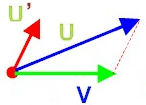
\includegraphics[scale=0.45]{addizione}
\caption{Schema della formula di addizione delle velocità}
\end{figure}
Siano allora $\theta'$ l’angolo tra $\textbf{u}'$ e $\textbf{v}$ e $\theta$ quello tra $\textbf{u}$ e $\textbf{v}$. Allora
\[
\sin \theta' = \frac{H}{u'}=\frac{H}{u}=\sin \theta
\]
e inoltre
\[
u'\cos \theta'=K \quad \cos\theta=\frac{v+K}{u} \to u\cos\theta-v=K
\]
Da queste relazioni si ottiene:
\begin{equation}
u'\sin\theta'=u\sin\theta \qquad u'\cos\theta'=u\cos\theta-v
\end{equation}
da cui
\begin{equation}
\frac{u'\sin\theta'}{u'\cos\theta'}=\frac{u\sin\theta}{u\cos\theta-v} \Longrightarrow \tan\theta'=\frac{\sin\theta}{\cos\theta-v/u}
\end{equation}
che, nel caso in cui $u=c$ e $v=v_{Terra}$ prende il nome di \textbf{formula dell'aberrazione stellare}. \\
Un'altra conseguenza importante della trasformazioni di Galileo riguarda il \emph{carattere assoluto dell'accelerazione}. Infatti:
\[
\textbf{a}'=\frac{d\textbf{u}'}{dt'}=\frac{d(\textbf{u}-\textbf{v})}{dt}=\frac{d\textbf{u}}{dt}=\textbf{a}
\]

\subsection{I due nuotatori}
\emph{Un nuotatore, capace di una velocità $c$ in acqua ferma, procede in un fiume per $L$ metri contro una corrente di velocità $v$, e torna poi al punto di partenza con la corrente a favore. Un secondo nuotatore di pari abilità attraversa il fiume ortogonalmente, con andata e ritorno da riva, percorrendo anch'egli una distanza $L$. Chi dei due termina per primo la gara?}
\\ \\
Denotiamo con $T_{\perp}$ il tempo impiegato dal nuotatore che si muove tra le sponde (nuotatore \textbf{1}) e con $T_{//}$ quello impiegato dal nuotatore che si muove prima contro e poi con la corrente (nuotatore \textbf{2}). Abbiamo che:
\[
T_{//}=\frac{L}{c-v}+\frac{L}{c+v}=\frac{2L}{c}\frac{1}{1-v^2/c^2}
\] 
Per quanto riguarda il nuotatore \textbf{2}, invece, questis i muoverà con velocità $v$ diagonalmente, e dunque, indipendentemente dal fatto che stia andando o tornando, la sua velocità effettiva sarà data da $\sqrt{c^2-V^2}$. Dunque:
\[
T_{\perp}=\frac{2L}{\sqrt{c^2-v^2}}=\frac{2L}{c}\frac{1}{\sqrt{1-v^2/c^2}}
\]
Dunque
\[
\frac{T_{\perp}}{T_{//}}=\sqrt{1-\frac{v^2}{c^2}}
\]
Osserviamo subito che il problema risulta indeterminato nel caso in cui $c\leq v$. In caso contrario, ovvero $c>v$, la gara viene vinta dal nuotatore \textbf{1}. 

\subsection{Equazioni del moto di Newton}
L'esempio paradigmatico di sistema dinamico è dato dalle equazioni del moto di Newton per $N$ punti materiali soggetti a forze centrali, cioè:
\[
m_a \frac{d^2x_a^i}{dt^2}=-\frac{\partial V}{\partial x_a^i}(x_1,\ldots,x_{3N})
\]
dove 
\[
V(\textbf{x}_1,\ldots,\textbf{x}_N)=\sum_{a\leq b} U(\left\| \textbf{x}_a-\textbf{x}_b \right\|)
\]
Possiamo notare che queste equazioni risultano evidentemente invarianti per traslazioni spaziali e dunque dalla soluzione del problema non è possibile ricavare la posizione dell'origine del sistema. L'invarianza per traslazioni temporali, invece, non è immediatamente ovvia: è necessario trovare una legge di trasformazione per \emph{funzioni} del tempo, e non del tempo stesso. Si potrebbe scrivere:
\[
x_a^i(t')=x_a^i(t-\tau)
\]
da cui
\[
\frac{dx_a^i(t')}{dt'}=\frac{dx_a^i(t)}{dt}=\frac{dx_a^i(t-\tau)}{dt}
\]
Da questa trasformazione è evidente che le traslazioni temporali sono simmetrie per il sistema se e soltanto se il sistema è isolato: infatti, nel caso di un potenziale dipendente dal tempo, la nostra affermazione non sarebbe corretta. A questo punto, dunque, l'invarianza delle equazioni di Newton per trasformazioni di Galileo è evidente: essendo il potenziale invariante per rotazioni (dipende solo dalla norma della distanza $\left\| \textbf{x}_a-\textbf{x}_b \right\|$, che è invariante per rotazioni), così come il gradiente del potenziale, che, in quanto traccia della matrice Jacobiana, è invariante per cambi di base. Infine, è necessario osservare che, nella dinamica Newtoniana, scelto un corpo standard che fornisca un'unità di massa, le altre masse possono essere determinate utilizzando il principio di azione e reazione: dunque le masse, così come le accelerazioni e di conseguenza le forze, hanno un carattere assoluto. Ovviamente l'invarianza (o meglio, \textbf{covarianza} - la dipendenza funzionale dalle variabili non viene alterata dal gruppo di trasformazioni) rispetto al gruppo di Galileo non si avrebbe se $R$, $\textbf{v}$ e $\textbf{a}$ dipendessero dal tempo. 

\subsection{Il fluido perfetto e la conduzione del calore}
Un secondo esempio di equazioni invarianti per trasformazioni di Galileo è fornito dal moto isoentropico di un fluido perfetto. Le equazioni sono:
\[
\frac{\partial u^i}{\partial t}+\textbf{u}\cdot \nabla u^i=-\frac{1}{\varrho}\frac{\partial P}{\partial x^i} 
\]
dove $\textbf{u}(\textbf{x},t)$ è il campo di velocità del fluido, $P$ è la pressione e $\varrho$ la densità di massa, soddisfacente all'equazione di continuità
\[
\frac{\partial \varrho}{\partial t}+\Div(\varrho\textbf{u})=0
\]
Per chiudere il sistema di equazioni deve anche essere assegnata un'equazione si stato, esprimente $P$ in funzione di $\varrho$, come ad esempio l'equazione baroentropica: 
\[
P=(\gamma-1)\varrho
\]
Il boost di Galileo agisce sui fluidi secondo la seguente trasformazione:
\[
u'^i(x',t)=u(x'^i+v^it,t)-v^i
\]
dove stiamo adottando un punto di vista \textbf{passivo}, ovvero il cambiamento dello stato è attribuito in questo caso al cambiamento dell'osservatore e non ad un reale cambiamento dello stato (punto di vista \textbf{attivo}). Infatti, in questo caso, il punto di vista attivo sarebbe da applicarsi nel caso in cui il fluido venisse materialmente spostato. La legge di trasformazione che abbiamo scritto rispecchia l'idea intuitiva che la velocità del fluido non può variare se non a causa del fatto che l'osservatore che la misura sia in moto relativo rispetto al fluido stesso. Inoltre:
\[
\varrho'(x'^i,t)=\varrho (x'^i+v^it,t) \qquad P'(x'^i,t)=P(x'^i+v^it,t)
\]
cioè il moto relativo del sistema di riferimento rispetto al fluido non deve influenzare la densità e la pressione del fluido stesso. Ora è facile dimostrare che le equazioni del moto del fluido sono covarianti galileiane. Scriviamo l'equazione in notazione tensoriale per un sistema di riferimento $\textbf{F}'$ in moto rispetto al fluido con velocità $\textbf{v}$:
\[
\frac{\partial u'^i}{\partial t}+\sum_{k=1}^3 u'^k \frac{\partial u'^i}{\partial x'^k}=-\frac{1}{\varrho'}\frac{\partial P'}{\partial x'^i} 
\]
Abbiamo che:
\[
\frac{\partial u'^i}{\partial t}(\textbf{x}',t)=\frac{\partial u^i}{\partial t}+\sum_{k=1}^3 v^k \frac{\partial u^i}{\partial x^k}=\frac{\partial u^i}{\partial t}+\textbf{v}\cdot \nabla \textbf{u}
\]
e inoltre
\[
\sum_{k=1}^3 u'^k \frac{\partial u'^i}{\partial x'^k}=\sum_{k=1}^3(u^k-v^k)\frac{\partial u^i}{\partial x^k}=\sum_{k=1}^3 u^k \frac{\partial u^i}{\partial x^k}-\textbf{v}\cdot \nabla \textbf{u}
\]
Quindi, ricostruendo l'equazione, la parte dipendente dalla velocità di traslazione del sistema di riferimento si semplifica, da cui l'invarianza. 
\\ \\
L'equazione della propagazione del calore in un corpo solido immobile diventa, nel caso 
semplice di corpi omogenei e isotropi, la seguente equazione per la distribuzione della 
temperatura $T$ nel corpo:
\[
\frac{\partial T}{\partial t}=\chi \nabla ^2 T
\] 
dove $\chi$ è la conducibilità termica. Se $T$ è un campo scalare, cioè se
\[
T'(\textbf{x}',t)=T(\textbf{x}+\textbf{v}t,t)
\]
allora si vede subito che l'equazione del calore non è invariante, in quanto
\[
\frac{\partial T'}{\partial t}=\frac{\partial T}{\partial t}+\textbf{v}\cdot \boldsymbol{\nabla} T
\]
Infatti il termine di trasporto può essere eliminato soltanto se nell'equazione originale vi è un termine di trasporto analogo. Deduciamo da questo che l'equazione del calore per un corpo in movimento con velocità $\textbf{u}$ deve essere corretta per come segue:
\[
\frac{\partial T}{\partial t}+\textbf{u}\cdot \boldsymbol{\nabla} T=\chi \nabla ^2 T
\]
Con questa correzione, e tenendo conto del fatto che $\textbf{u}=\textbf{u}'+\textbf{v}$ per la legge di addizione delle velocità, abbiamo la covarianza dell'equazione. 
\\
Dal punto di vista delle rappresentazioni del gruppo di Galilei, il \textbf{quadrivettore} $q=(\dot{T},\boldsymbol{\nabla}T)$ si trasforma secondo una delle due possibili rappresentazioni quadrivettoriali del gruppo: detto $(\eta,\boldsymbol{\chi})$ il quadrivettore generico, si ha:
\begin{enumerate}[i.]
	\item $\eta'=\eta+\textbf{v}\cdot \boldsymbol{\chi}$, $\boldsymbol{\chi}'=\boldsymbol{\chi}$;
	\item $\eta'=\eta$, $\boldsymbol{\chi}'=\boldsymbol{\chi}+\eta\textbf{v}$.
\end{enumerate}

\subsection{L'equazione di Schr\"{o}dinger}
Nel caso di una particella libera, l'equazione di Schr\"{o}dinger che sostituisce la legge classica $\dot{\textbf{v}}=0$ è, se $\hbar=1$:
\[
i\frac{\partial \Psi}{\partial t}=-\frac{1}{2m}\nabla^2\Psi
\]
L'invarianza per traslazioni e rotazioni è evidente se si definisce la trasformazione attiva della funzione d'onda nel seguente modo (e ricordando inoltre che il laplaciano è invariante per rotazioni in quanto traccia della matrice Hessiana):
\[
\Psi'(\textbf{x},t)=\Psi(R\cdot \textbf{x}+\textbf{a},t+\tau)
\]
Osserviamo che l'applicazione $\Psi \mapsto \Psi'=U(R)\psi$ è unitaria:
\[
(\Psi,\Phi)=\int d^3x \Psi(\textbf{x})\Phi(\textbf{x})=\int d^3x U(R)\Psi(\textbf{x})U(R)\Phi(\textbf{x})=(U(R)\Psi,U(R)\Phi)
\]
Consideriamo ora il boost $\textbf{x}'=\textbf{x}-\textbf{v}t$. L'equazione di Schr\"{o}dinger è evidentemente NON invariante rispetto a questa trasformazione, ed inoltre non è possibile inserire un termine dipendentemente dalla velocità, in quanto, a causa del principio di indeterminazione, la velocità della particella non ha significato in meccanica quantistica. L'unica possibilità risiede dunque nell'appellarsi alla fase arbitraria delle funzioni d'onda. Definiamo allora:
\begin{equation}\label{eq:sch}
\Psi'(\textbf{x},t)=e^{-i\frac{mv^2}{2}t+m\textbf{v}\cdot \textbf{x}}\Psi(\textbf{x}+\textbf{v}t,t)
\end{equation}
$\Psi'$ soddisfa ancora l'equazione di Schr\"{o}dinger, e inoltre la trasformazione $\Psi\mapsto\Psi'$ è unitaria. Dunque la meccanica quantistica per la particella libera è Galilei-invariante. 
\\
La formula di trasformazione (\ref{eq:sch}) introduce una fase che dipende dalla velocità relativa. E' quindi interessante osservare che se fosse possibile misurare la fase relativa di due particelle con masse diverse allora, effettuando un boost, si potrebbe misurare la velocità relativa di due riferimenti inerziali. Infatti:
\[
\varphi_{relativa}=e^{i\Delta m \textbf{v}\cdot \textbf{x}}
\]
si dice allora che la simmetria galileiana, o il principio di relatività, impone una \textbf{regola di superselezione della massa}, per cui non è possibile preparare combinazioni lineari di stati descriventi particelle con masse diverse, e di conseguenza non dev'essere possibile misurare la fase relativa di particelle con masse diverse. 
\\ \\
La formula di trasformazione (\ref{eq:sch}) sembra scritta ad hoc per avere la 
covarianza dell'equazione di Schr\"{o}dinger. Naturalmente il fatto notevole è che una tale 
formula esista, e ci si può chiedere allora se non vi sia un modo sistematico per trovare 
le formule di trasformazione in casi più complicati. La materia che si occupa di questi 
problemi è una teoria matematica nota come \textbf{teoria della rappresentazione dei gruppi}. Essa 
fornisce la classificazione delle formule di trasformazione possibili e determina il carattere 
delle grandezze che si trasformano o, come si suol dire, lo spazio della rappresentazione. 

\begin{defn}
Una \textbf{rappresentazione} di un gruppo $\mathcal{G}$ su uno spazio vettoriale $V$ è un omomorfismo di gruppi $\rho:\mathcal{G}\to\gl$, dove $\gl$ è detto \textbf{gruppo generale lineare}, ovvero il gruppo degli operatori invertibili sullo spazio vettoriale $V$. $V$ è detto \textbf{spazio di rappresentazione} e $n=\dim V$ \textbf{dimensione della rappresentazione}. Diremo che una rappresentazione è \textbf{fedele} se è iniettiva. 
\end{defn}

\section{Ottica non relativistica}
Nuove opportunit`a e nuovi problemi sorgono per`o in relazione ai fenomeni connessi con 
la propagazione della luce. Infatti le equazioni di Maxwell non hanno la proprietà di 
covarianza richiesta dal principio di relatività galileiano, cioè non sono invarianti per 
trasformazioni di Galilei. Per capirlo basta notare che la velocit`a di un impulso elettromagnetico dipende dal sistema di riferimento, se vale la (4.1), mentre le equazioni di 
Maxwell predicono che sia indipendente dal moto della sorgente e uguale alla costante 
universale c che compare nelle equazioni stesse. \\
Lo stesso Maxwell pensava che le sue equazioni valessero in una classe limitata di sistemi 
di riferimento, quelli in quiete rispetto al cosiddetto etere, una sostanza imponderabile 
ed elastica presente nell'universo, che si credeva propagasse la luce e rendesse possibili i 
fenomeni elettromagnetici, alla stessa maniera che un gas `e necessario per la propagazione 
del suono. \\
Ma se è così allora dovrebbe essere possibile misurare la velocità assoluta della terra, 
perchè il suo moto attraverso l'etere causerebbe un “drift” in grado di alterare la velocità 
della luce a seconda della sua direzione di propagazione. \\
Ma se non sappiamo quali sono le equazioni elettromagnetiche in un riferimento mobile, 
come si possono trattare i fenomeni elettromagnetici in un riferimento terrestre, in movimento rispetto all'etere? La maniera più semplice e diretta è determinare l'effetto del 
gruppo di Galilei sulle caratteristiche di un'onda elettromagnetica piana. 

\newpage

\subsection{Onde piane e velocità di fase}

\newpage

\subsection{La velocità di gruppo}

\newpage

\subsection{La velocità della luce nei dielettrici trasparenti}

\newpage

\subsection{L'aberrazione e l'effetto Doppler}

\newpage
.
\newpage

\section{Esperienze di fine secolo XIX}

\subsection{Hoek}

\newpage

\subsection{Fizeau e Fresnel}
\subsection{Michelson e Morley}

\newpage

\subsection{Interpretazioni}

\newpage

\section{Esperienze moderne}

\chapter{Fondamenti di relatività speciale}

\section{L'equazione delle onde}
Nonostante la meccanica risulti invariante per trasformazioni di Galileo, lo stesso non vale per l'equazione delle onde. Infatti:
\[
\frac{1}{c^2}\frac{\partial^2f}{\partial t^2}-\nabla^2f=0
\]
è non invariante rispetto al gruppo di Galileo. Ci chiediamo allora: qual è il suo gruppo di invarianza, se ne ha uno? Per lo scopo, introduciamo le nuove variabili $x^1=x$ e $ix^2=ct$, con $i$ l'unità immaginaria e $1,2$ apici e non esponenti. Così facendo, possiamo riscrivere l'equazione in questa maniera:
\[
\frac{\partial^2f}{\partial (x^1)^2}+\frac{\partial^2f}{\partial (x^2)^2}=\nabla^2f(x^1,x^2)=0
\]
Quanto abbiamo fatto è stato ricondursi all'equazione di Laplace bidimensionale, il cui gruppo di invarianza è dato da $SO(2)$. Dunque possiamo scrivere le seguenti trasformazioni di coordinate:
\[
\begin{cases}
x'^1=x^1\cos\alpha-x^2\sin\alpha \\
x'^2=x^1\sin\alpha+x^2\cos\alpha \\
\end{cases}
\]
Ripristinando le variabili iniziali si ha
\[
\begin{cases}
x'^1=x^1\cos\alpha+ict\sin\alpha \\
x'^2=x^1\sin\alpha-ict\cos\alpha \\
\end{cases}
\]
Per ripristinare l'equazione di partenza, che è a coefficienti reali, è necessario introdurre un angolo puramente immaginario $\alpha=i\psi$ da cui, valendo le uguaglianze $\sin(i\psi)=i\sinh\psi$, $\cos(i\psi)=\cosh\psi$, si ottiene
\begin{equation}\label{eq:gruppo}
\begin{cases}
x'^1=x^1\cosh\psi-ct\sinh\psi \\
ct'=-x^1\sinh\psi+ct\cosh\psi \\
\end{cases}
\end{equation} 
Dunque, se l'equazione di Laplace bidimensionale è invariante per rotazioni, allora l'equazione delle onde nel pianto $x,ct$ è invariante per il gruppo di rotazioni in (\ref{eq:gruppo}). Tale gruppo non è compatto (dove per compatto intendiamo una generalizzazione del concetto di gruppo finito), e viene indicato con $SO(1,1)$. Quindi, così come la norma di $\mathbb{R}^n$ è invariante per rotazioni, la forma quadratica
\[
s^2=-c^2t^2+(x^1)^2
\]
è invariante per rotazioni iperboliche. Diremo allora che il \textbf{gruppo di Lorentz} è il gruppo delle trasformazioni lineari omogenee dello spaziotempo che preservano $s^2$. 
\\
Per determinare $\psi$, osserviamo che il punto $x'^1=0$, cioè l'origine del sistema di riferimento in movimento $\textbf{F}'$, deve muoversi con velocità uniforme $v$. Cioè:
\[
0=x^1\cosh\psi-ct\sinh\psi \Longrightarrow v=c\tanh\psi
\]
Il parametro $\psi$ propriamente denota la \emph{rapidità} della trasformazione, poichè per $\psi\to\infty$ si ha $v\to c$. Inoltre, siccome:
\[
\cosh\psi=\frac{1}{\sqrt{1-\tanh^2\psi}}= \frac{1}{\sqrt{1-v^2/c^2}}\qquad \sinh\psi=\tanh\psi\cosh\psi=\frac{v/c}{\sqrt{1-v^2/c^2\psi}}
\]
possiamo riscrivere in definitiva:
\begin{equation}\label{eq:lorentz}
\begin{cases}
x'=\frac{x-vt}{\sqrt{1-v^2/c^2}}\\
ct'=\frac{t-(v/c)x}{\sqrt{1-v^2/c^2}}
\end{cases}
\end{equation}
dette \textbf{trasformazioni di Lorentz}. Introducendo il fattore
\[
\gamma=\frac{1}{\sqrt{1-v^2/c^2}}
\]
detto \textbf{gamma di Lorentz} o \textbf{fattore di Lorentz}, possiamo riscrivere (\ref{eq:lorentz}) come:
\[
\begin{cases}
x'=\gamma(x-vt) \\
ct'=\gamma(t-(v/c)x) \\
\end{cases}
\]

\section{Gli assiomi di Einstein}
Il persistente fallimento dei tentativi di rilevare una qualsiasi influenza del moto della 
terra sulla propagazione della luce è ovviamente incompatibile con l'esistenza di un ''etere 
imponderabile'' e conduce alla conclusione ''altamente probabile, se non certa'' (W. Pauli), 
che tutte le leggi del la fisica, inclusa l'elettrodinamica, obbediscano a un \emph{principio di 
relatività}. Fu A. Einstein che introdusse questo punto di vista relativistico moderno come il primo di 
due assiomi, il secondo dei quali, ''solo apparentemente incompatibile con il primo'', stabilisce anche che la velocità della luce sia la stessa in tutti i sistemi di riferimento inerziali. 
A questo proposito, si può osservare che le equazioni di Maxwell predicono che la velocità 
della radiazione elettromagnetica nel vuoto sia indipendente dal moto macroscopico della 
sorgente, e l'esperimento di Michelson e Morley è compatibile con questo fatto con una 
precisione del secondo ordine in $v/c$. Tuttavia essa potrebbe ancora dipendere da termini di ordine superiore in $v/c$. E' molto più semplice assumere, con Einstein, che la velocità della luce nel vuoto sia del tutto 
indipendente dal moto della sorgente e dell'osservatore. Citando direttamente Einstein:
\begin{enumerate}[i.]
	\item \emph{Primo principio}: Le leggi secondo le quali si modificano gli stati dei sistemi fisici sono 
indipendenti dal fatto che questi cambiamenti di stato vengano riferiti all'uno 
o all'altro di due sistemi di coordinate che si trovino in relativa reciproca 
traslazione uniforme. 

	\item \emph{Secondo principio}: ogni raggio di luce si muove nel sistema di coordinate ''in quiete'' con 
la determinata velocità $V$ , indipendente dal fatto che quel raggio di luce sia 
emesso da una sorgente in quiete, o da una sorgente in movimento. 
\end{enumerate}
Dal primo principio, nel sistema mobile in cui la sorgente è ferma la velocità della luce è ancora $c$, cosicché si 
potrebbe enunciare il secondo principio in questa versione equivalente:
\begin{enumerate}[iii.]
	\item \emph{Secondo principio}: la velocità della luce nel vuoto ha lo stesso valore in tutti i sistemi di 
riferimento inerziali, in ogni direzione, tempo e luogo.
\end{enumerate} 

\subsection{Osservazione sui postulati}
(i) Il principio di relatività da solo non è sufficiente a determinare un gruppo univoco 
di trasformazioni delle coordinate spazio-temporali. Infatti la meccanica newtoniana è 
covariante rispetto al gruppo di Galilei, mentre la meccanica relativistica lo è rispetto al 
gruppo di Lorentz. \\
Come ha mostrato Einstein però, gli assiomi primo e secondo sono sufficienti a determinare 
il gruppo di simmetria senza bisogno di assumere valida in tutti i sistemi inerziali l'intera 
teoria elettromagnetica di Maxwell, una semplificazione, questa, assai ragguardevole. Le 
equazioni della meccanica invece, invarianti galileiane, dovranno essere riformulate in 
modo tale da renderle compatibili con la nuova simmetria. La meccanica relativistica che 
ne risulta differisce molto poco da quella newtoniana (le correzioni sono tutte di ordine $v^2/c^2$, che è indubbiamente il motivo per cui non sono state scoperte prima) ma è indispensabile, per esempio, 
a trattare le particelle veloci che viaggiano nei moderni acceleratori di particelle e alcuni 
fenomeni di astrofisica relativistica, e ha collezionato numerose verifiche sperimentali. \\
(ii) Il carattere non ovvio del primo postulato, cioè del principio di relatività, si può 
apprezzare considerando il fatto che, in base ad esso, il moto uniforme del centro di 
massa dell'universo rispetto a un sistema qualunque non dovrebbe produrvi alcun effetto
osservabile. Evidentemente nessuno è in grado di verificare una simile asserzione e dunque, 
se non vogliamo introdurre argomenti metafisici nella meccanica, il principio di relatività 
ha un preciso significato fisico solo per i sistemi isolati. \\
Il problema è: quando si può dire che un sistema è isolato? L'esperienza mostra che per il 
moto uniforme è sufficiente assumere che tutte le masse siano adeguatamente distanti, ma 
che non può dirsi altrettanto per il moto accelerato. Nei sistemi accelerati appaiono infatti 
campi di forza apparentemente privi di cause, e che per tale motivo Newton ricondusse 
agli effetti dell'accelerazione assoluta, riferita cioè allo spazio assoluto. E' assai probabile 
che i campi inerziali dipendano invece dall'accelerazione rispetto ''alla massa della terra 
e degli altri corpi celesti'' (espressione usata da Mach), la sola che ha significato fisico, 
secondo Mach, e in ogni caso la sola che si può osservare. \\
(iii) Il ruolo principale del secondo assioma, con il suo riferimento esplicito alla velocità della 
luce, non è tanto quello di suggerire un ruolo speciale o privilegiato del campo elettromagnetico in 
natura, quanto quello di stabilire l'esistenza di una velocità limite insuperabile. Infatti dei 
due casi, che una velocità limite esista, o che non esista, solo il primo implica la simmetria 
di Lorentz. Ma il valore della velocità limite, che proprio in virtù di tale proprietà deve 
essere la stessa in tutti i sistemi di riferimento, non è fissato da questo argomento. Il 
secondo postulato fissa precisamente questo valore, riconducendolo alla velocità della luce 
nel vuoto. \\

\subsection{La definizione del tempo}
Il problema spinoso è come confrontare il tempo di eventi che accadono in luoghi diversi. 
Il problema sorge perché se le leggi fisiche sono locali e la velocità dei segnali è limitata, la 
definizione del tempo comune a eventi in luoghi diversi necessita di una \emph{convenzione per 
sincronizzare gli orologi}. Prima dell'avvento della teoria di Einstein, questo era considerato essenziale un problema di ordine tecnico, più che una questione fortemente concettuale. Ad esempio, per stabilire se due orologi identici separati da una 
certa distanza indichino lo stesso tempo, si può inviare un raggio di luce dal primo verso 
il secondo e regolare quest'ultimo in base al ritardo dovuto alla velocità di propagazione 
finita del segnale. Ma questa procedura richiede ovviamente che si conosca il valore della 
velocità della luce (che si può determinare con misure puramente elettromagnetiche); in altri termini, la velocità della luce deve essere nota se vogliamo 
sincronizzare gli orologi, benché si richiedano orologi preventivamente sincronizzati per 
determinare la velocità della luce. Anche il trasporto di un orologio da un punto all'altro 
incontra la stessa difficoltà: per correggere i possibili effetti del trasporto, si deve disporre 
di orologi preventivamente sincronizzati. I tempi degli eventi, pertanto, non possono 
essere confrontati prima che si sia stabilita una procedura per sincronizzare gli orologi, 
ossia prima che si sia stabilito che cosa si intende per ''tempo comune a eventi distanti''. 
Secondo il metodo di Einstein, il tempo comune di due eventi $A$ e $B$ può essere definito 
quando si stabilisca, per definizione, che il tempo che la luce impiega per viaggiare da 
$A$ a $B$ è uguale al tempo che impiega per tornare da $B$ ad $A$. Quindi se il raggio parte 
all'istante $t_A$ da A, giunge in B all'istante $t_B$ (misurato ''vicino'' a B), e ritorna in A 
all’istante $t'_A$ (misurato vicino ad A), si avrà l’equazione:
\begin{equation}\label{eq:tempo}
t'_A-t_B=t_B-t_A
\end{equation}
(un caso più generale si ha ponendo $t'_A-t_B=t'_B-t_A$ dove si assume che la partenza del segnale da 
$B$ non coincida necessariamente con il suo arrivo da $A$). Diremo che due orologi sono \textbf{sincroni} se la relazione (\ref{eq:tempo}) è valida. Con questo si è innanzitutto definito un criterio per decidere quando due orologi distanti sono sincroni, ma non solo. Dall'uguaglianza dei tempi di andata e ritorno del segnale si deduce l'uguaglianza 
della velocità della luce all'andata con la velocità della luce al ritorno: cioè, detta $L_{AB}$ la 
distanza tra $A$ e $B$, si ha
\begin{equation}\label{eq:luce}
c=\frac{L_{AB}}{t_B-t_A}=\frac{L_{AB}}{t'_A-t_B}
\end{equation} 
 Chiaramente (\ref{eq:luce}) non è oggetto di verifica sperimentale, e verrà chiamata \textbf{one-way velocity of light}. Con questo si assume però 
che la velocità della luce sia la stessa per tutte le coppie di orologi sincronizzati, un dato 
che non segue logicamente dalla definizione di Einstein (perchè sia vero è necessario supporre che il tempo sia isotropo e omogeneo), che, si noti, che non dipende dal valore numerico di c. Dalla (\ref{eq:tempo}) segue anche che:
\[
c=\frac{2L_{AB}}{t'_A-t_A}
\]
detta \textbf{two-way velocity of light}. 
\\
\\
Se un raggio luminoso segue un percorso poligonale chiuso con lati $l_i$, si può misurare il 
tempo di volo con un unico orologio. Cioè se
\begin{equation}\label{eq:fizeau}
c=\frac{\sum_i l_i}{T}
\end{equation}
allora si può mostrare che un orologio $O$ è sincronizzato con orologi identici $A$ e $B$ se e solo se questi sono sincronizzati tra di loro. Chiameremo $O$ \textbf{orologio regolatore}: quanto andremo a dimostrare ci assicura, dunque, che la procedura di sincronizzazione degli orologi non dipende dall'orologio regolatore. Consideriamo allora i tre orologi $O$, $A$, $B$ rispettivamente distanti $l_0$, $l_1$ ed $l_2$ e facciamo partire un segnale da $O$ in $t_O$, che, per sincronia, arriverà in $A$ al tempo
\[
t_A=t_O+\frac{l_0}{c}
\]
se $l_0$ è la lunghezza del percorso che divide $O$ da $A$. A questo punto, il segnale viene trasmesso in $B$, dove giunge al tempo $t_B=t$ e da dove viene riflesso per tornare in $O$ al tempo
\[
t'_O=t+\frac{l_2}{c}
\]
Quanto vogliamo dimostrare, allora, è che
\[
t=t_A+\frac{l_1}{c}
\]
La deduzione di questo risultato non può essere puramente matematica, ma è necessario tirare in ballo il risultato dell'esperimento di Fizeau, che dà una prova diretta di (\ref{eq:fizeau}). Quindi
\[
t'_O=t+\frac{l_2}{c}=t_O+\frac{l_0+l_1+l_2}{c}
\]
da cui
\[
t=t_O+\frac{l_0+l_1}{c}=\left( t_O +\frac{l_0}{c}\right)+\frac{l_1}{c}=t_1+\frac{l_1}{c}
\]
Conseguentemente il metodo di Einstein è dunque libero da contraddizioni logiche. 
\\
Il tempo comune di eventi distanti è adesso definito da orologi sincronizzati posti nelle 
immediate vicinanze degli eventi, trascurando l'inesattezza che deriva dal fatto che gli 
orologi non coincidono esattamente con gli eventi. In particolare gli eventi $A$ e $B$ si 
diranno \textbf{simultanei} se gli orologi suddetti indicano lo stesso tempo. 
La procedura descritta deve essere applicata a tutti i sistemi di riferimento inerziali, con 
gli orologi in quiete nei rispettivi sistemi. Ogni riferimento inerziale avrà quindi il suo 
proprio tempo, definito da orologi sincronizzati che occupano posizioni fisse, e in tali 
sistemi la velocità della luce risulterà per definizione costante, isotropa e numericamente 
uguale a $c$. Non è detto, a priori, che questi tempi concordino per tutti gli osservatori 
inerziali. 

\section{Le trasformazioni di Lorentz}
Data la definizione del tempo in un sistema inerziale, passiamo ora a determinare il gruppo 
di trasformazioni delle coordinate spazio-temporali che è in accordo con questa definizione 
e con il principio di relatività. 

\subsection{Condizioni sulle trasformazioni}
E' conveniente introdurre la notazione $x^a$, $a\in\{0,1,2,3\}$ per indicare le coordinate, con la corrispondenza $x^0=ct$, $x^1=x$, $x^2=y$, $x^3=z$. Le trasformazioni richieste devono avere la proprietà di conservare i moti uniformi, e se assumiamo che i sistemi di riferimento coincidano per $t=t'=0$, allora devono essere funzioni lineari delle coordinate, cioè della forma
\[
x'^a=\sum_{a=0}^3L^a_bx^b
\]
dove abbiamo utilizzato la convenzione riguardante la somma su indici ripetuti. L'assioma (\emph{ii}.) indica che l'equazione di un fronte d'onda sferico nel sistema di riferimento inerziale \textbf{F}
\[
-c^2(t-t_0)^2+(x-x_0)^2+(y-y_0)^2+(z-z_0)^2=0
\]
è la stessa del fronte d'onda in \textbf{F}'
\[
-c^2(t'-t'_0)^2+(x'-x'_0)^2+(y'-y'_0)^2+(z'-z'_0)^2=0
\]
Quanto ci chiediamo ora è come trovare delle trasformazioni di coordinate che posseggano questa proprietà: se richiediamo che le trasformazioni siano lineari
\begin{align*}
&-c^2(t'-t'_0)^2+(x'-x'_0)^2+(y'-y'_0)^2+(z'-z'_0)^2= \\
&=\lambda(L)[-c^2(t-t_0)^2+(x-x_0)^2+(y-y_0)^2+(z-z_0)^2]
\end{align*}
dove $\lambda(L)$ è in generale una funzione della matrice di trasformazione $L_a^b$. Se $L$ è una rotazione, nel senso che $L_i^0=L_0^i=0$ e $L_j^i\in O(3)$, allora $\lambda(L)=1$ e $\lambda(L)\lambda(L')=\lambda(LL')$. Semplici trasformazioni che lasciano invariante il cono di luce sono le traslazioni spaziotemporali
\[
t'=t+a^0/c \quad \textbf{x}'=\textbf{x}+\textbf{a}
\]
le trasformazioni di scala
\[
x'_a=\lambda x^a \quad \lambda>0
\]
e le rotazioni delle coordinate
\[
x'^i=\sum_{j=1}^3 R^i_j x^j \quad t'=t
\]
Le due ultime trasformazioni sono lineari e omogenee, ma non cambiano la velocità relativa dei sistemi di riferimento. Le simmetrie di rotazione e traslazione corrispondono all'isotropia e omogeneità dello spazio e sono associate a importanti leggi di conservazione, sperimentalmente verificate. Le trasformazioni di scala, invece, non rappresentano simmetrie delle leggi fisiche note: occorre precisare, infatti, che le dilatazioni non modificano le masse o le costanti di accoppiamento delle interazioni, e quindi l'invarianza di scala è possibile solo se tutte le masse sono nulle o se formano uno spettro continuo e se le costanti di accoppiamento sono adimensionali. 

\subsection{Trasformazioni speciali}
Basandoci sul sistema (\ref{eq:lorentz}), concludiamo che la matrice corrispondente alle trasformazioni di Lorentz è data da:
\[
L(v)=
\left(
\begin{array}{cccc}
\gamma & -\gamma v/c & 0 & 0 \\
-\gamma v/c & \gamma & 0 & 0 \\
0 & 0 & 1 & 0 \\
0 & 0 & 0 & 1 \\
\end{array} \right)
\]
Ponendo $\gamma\equiv \gamma(v)$, possiamo osservare che:
\begin{align*}
\gamma(v)\gamma(v')&=\frac{1}{\sqrt{1-v^2/c^2}}\frac{1}{\sqrt{1-v'^2/c^2}}=\frac{1}{\sqrt{1-v'^2/c^2-v^2/c^2+v'^2v^2/c^4}}= \\
&=\frac{1}{\sqrt{1-\frac{v'^2+v^2}{c^2}+\frac{v'^2v^2}{c^4}}}= \frac{1}{\sqrt{1+\frac{v'^2v^2}{c^4}+\frac{2v'v}{c^2}-\frac{v'^2+v^2}{c^2}-\frac{2v'v}{c^2}}}= \\
&= \frac{1}{\sqrt{\left( 1+\frac{v'v}{c^2} \right)^2-\left( \frac{v'+v}{c^2} \right)^2}}=\frac{1}{\left( 1+\frac{v'v}{c^2} \right)\sqrt{1-\frac{\left( \frac{v'+v}{c} \right)^2}{\left( 1+\frac{v'v}{c^2} \right)^2}}}
\end{align*}
Osserviamo che
\[
\frac{\left( \frac{v'+v}{c} \right)^2}{\left( 1+\frac{v'v}{c^2} \right)^2}=\frac{1}{c^2}\frac{(v'+v)^2}{(1+\frac{v'v}{c^2})}\equiv \frac{w^2}{c^2}
\]
e dunque
\[
\gamma(v)\gamma(v')\left( 1+\frac{v'v}{c^2} \right)=\gamma(w)
\]
Il prodotto di due trasformazioni di Lorentz collineari con velocità $v$ e $v'$ è quindi dato da:
\begin{align*}
L(v)L(v')&=
\left(
\begin{array}{cccc}
\gamma(v) & -\gamma(v) v/c & 0 & 0 \\
-\gamma(v) v/c & \gamma(v) & 0 & 0 \\
0 & 0 & 1 & 0 \\
0 & 0 & 0 & 1 \\
\end{array} \right)
\left(
\begin{array}{cccc}
\gamma(v') & -\gamma(v') v'/c & 0 & 0 \\
-\gamma(v') v'/c & \gamma(v') & 0 & 0 \\
0 & 0 & 1 & 0 \\
0 & 0 & 0 & 1 \\
\end{array} \right)= \\
&=\left( \begin{array}{cccc}
\gamma(v)\gamma(v')(1+v'v/c^2) & -\gamma(v)\gamma(v') (v'+v)/c & 0 & 0 \\
-\gamma(v)\gamma(v') (v'+v)/c & \gamma(v)\gamma(v')(1+v'v/c^2) & 0 & 0 \\
0 & 0 & 1 & 0 \\
0 & 0 & 0 & 1 \\
\end{array} \right)=\\
&=\left(
\begin{array}{cccc}
\gamma(w) & -\gamma(w) w/c & 0 & 0 \\
-\gamma(w) w/c & \gamma(w) & 0 & 0 \\
0 & 0 & 1 & 0 \\
0 & 0 & 0 & 1 \\
\end{array} \right)
\end{align*}
Cioè
\[
L(v)L(v')=L(w)
\]
A questo punto, avendo eliminato le dilatazioni, possiamo mostrare che non ci sono altri fattori $\lambda\textbf{v})$ al di fuori di $\lambda(\textbf{v})=1$. Infatti, avendo 
\[
\lambda(\textbf{v})\lambda(\textbf{v}')=\lambda(\textbf{w})
\]
deve essere vero che
\[
\lambda(\textbf{v})\lambda(-\textbf{v})=\lambda(\textbf{w})=\lambda\left(\frac{\textbf{v}-\textbf{v}'}{1+\textbf{v}\cdot\textbf{v}'/c^2}\right)=\lambda(0)=1
\]
poichè necessariamente $\lambda(0)=1$ (cioè la trasformazione per velocità relativa nulla si riduce all'identità). Consideriamo ora $R_{\pi}$ una rotazione che inverte $\textbf{v}=v\hat{\textbf{x}}$, cioè $R_{\pi}\textbf{v}=-\textbf{v}$. Allora:
\[
\lambda(-\textbf{v})=\lambda(R_{\pi}\textbf{v})=\lambda(R_{\pi})\lambda(\textbf{v})=\lambda(\textbf{v})
\]
In conclusione si deve avere
\[
\lambda(\textbf{v})=1
\]
\subsection{La più generale trasformazione di Lorentz}
Le quattro coordinate di un evento in un sistema di riferimento inerziale identificano un punto dello spazio-tempo. Ad ogni sistema \textbf{F} , \textbf{F}',$\ldots$, \textbf{F}$^{(n)}$ è associato il proprio sistema di coordinate $\{x^a\}$, $\{x'^a\}$,$\ldots$, $\{x^{(n)a}\}$, per mezzo del quale si possono identificare gli eventi. L'insieme degli eventi in relatività ristretta prende anche il nome di \textbf{spaziotempo di Minkowski}. Dunque trasformazioni di Lorentz sono interpretabili come applicazioni 
lineari operanti sullo spazio di Minkowski. Si noti che i quattro numeri $\{x^a\}$, $a\in\{0,1,2,3\}$ definiscono ciò che in algebra si chiama un \textbf{quadri-vettore}, le cui componenti si trasformano linearmente per effetto di una 
''rotazione'' dei vettori di base. \\
Sottolineiamo il fatto essenziale che le coordinate devono essere definite operativamente. Ad esempio, il tempo di ogni evento è indicato da un orologio ''vicino'' all'evento e sincronizzato agli altri orologi dalla procedura indicata precedentemente, mediante l'invio di segnali elettromagnetici. Non è affatto scontato che lo spazio-tempo, inteso come 
l'insieme di tutti gli eventi, abbia la struttura di spazio vettoriale caratteristica della relatività speciale, né questa struttura deriva logicamente dalla sua definizione euristica come 
\emph{insieme di tutti gli eventi}. Tuttavia questo è ciò che si osserva localmente. \\ \\
Abbiamo visto che le trasformazioni di Lorentz non cambiano il valore della forma quadratica che rappresenta l'intervallo spaziotemporale tra due eventi:
\begin{equation}\label{eq:inter}
ds^2=-(x^0-y^0)^2+\sum_{i=1}^3(x^i-y^i)^2
\end{equation}
Introducendo la \textbf{metrica} diagonale $\eta_{ab}=\eta_{ba}$ tale che $\eta_{00}=-1$ e $\eta_{ij}=\delta_{ij}$, ovvero
\[
\eta_{ab}=
\left( \begin{array}{cccc}
-1 & 0 & 0 & 0 \\
0 & 1 & 0 & 0 \\
0 & 0 & 1 & 0 \\
0 & 0 & 0 & 1 \\
\end{array}\right)
\]
si ha che il secondo membro di (\ref{eq:inter}) può essere scritto utilizzando il \textbf{prodotto scalare} indotto dalla metrica:
\[
(x,y)=\eta_{ab}x^ay^b
\]
cioè come $(x-y,x-y)=(x,x)+(y,y)-2(x,y)$. Chiaramente il prodotto scalare appena definito è bilineare e non degenere (cioè $(x,y)=0 \leftrightarrow x=0,y=0$), ma non definito positivo. \\
Siccome le trasformazioni di Lorentz lasciano invariato l'intervallo spaziotemporale, possiamo definirle come elementi del gruppo delle isometrie dello spazio di Minkowski, gruppo che indicheremo con il simbolo $\mathcal{L}$. In altri termini, si tratta di trasformazioni di coordinate lineari e omogenee
\[
x^a \to x'^a=\Lambda_b^ax^b
\]
che preservano il prodotto scalare, cioè
\[
(\Lambda x,\Lambda y)=(x,y)
\]
Di conseguenza, per non degenerazione del prodotto scalare si deve avere
\[
\eta_{ab}x^ay^b=(x,y)=(\Lambda x,\Lambda y)=\eta_{cd}\Lambda_a^c x^a\Lambda_b^d y^b
\]
ovvero
\[
\eta_{ab}=\eta_{cd}\Lambda_a^c \Lambda_b^d
\]
Consideriamo a questo punto una trasformazione di Lorentz generica:
\[
x'^a=\sum_{a=0}\Lambda_a^b x^b
\]
e applichiamola al vettore $e^a=(1,0,0,0)$, ovvero quel vettore tale che $(e,e)=-1$. Si avrà:
\[
x'^a = \sum_{a=0}^3\Lambda_a^b x^b=\sum_{a=0}^3 \Lambda _a ^0 x^0
\]
cioè otterremo un vettore del tipo
\[
\Lambda\cdot e = (x,\textbf{x})
\]
tale che $-x^2+|\textbf{x}|^2=-1$, per conservazione del prodotto scalare. Sia ora $R$ una rotazione che riporta il vettore lungo l'asse $\hat{x}$:
\[
R\cdot \Lambda \cdot e = (x,|\textbf{x}|,0,0)
\]
Ora, siccome $x>|\textbf{x}|$, ponendo $u=|\textbf{x}|/x$ ($c=1$) e applicando il boost $L(u)$ otteniamo che:
\[
\begin{cases}
x'=\gamma (x-u|\textbf{x}|) \\
|\textbf{x}|'=\gamma (|\textbf{x}|-ux)
\end{cases}
\]
Osserviamo subito che
\[
|\textbf{x}|'=\gamma\left(|\textbf{x}|-\frac{|\textbf{x}|}{x}x\right)=0
\]
Inoltre:
\[
x'=\gamma(x-u|\textbf{x}|)=\gamma \left( x-\frac{|\textbf{x}|}{x}|\textbf{x}| \right)=x\gamma(x^2-|\textbf{x}|^2)=x\gamma
\]
dove 
\[
\gamma = \sqrt{1-\frac{|\textbf{x}|^2}{x^2}}=\frac{1}{x}\sqrt{x^2-|\textbf{x}|^2}=\frac{1}{x}
\]
da cui $x'=1$. Di conseguenza
\[
L(u)\cdot R \cdot \Lambda \cdot e = e
\]
da cui otteniamo che, necessariamente, $R'=L(u)\cdot R \cdot L$ è una rotazione spaziale. Ma allora:
\[
\Lambda=R^{-1}\cdot L(-u) \cdot R'
\]
è la più generale trasformazione di Lorentz propria ($\det \Lambda = 1$) e ortocrona ($\Lambda_0^0 \geq 0$). 
\subsection{Intervalli spaziali e temporali}
Dalle trasformazioni di Lorentz si ricava che un regolo (asta rigida) in moto con velocità $v$ in un riferimento \textbf{F}  e avente \textbf{lunghezza propria} $L_0$ (la lunghezza nel riferimento \textbf{F}' nel quale il regolo è in quiete) ha lunghezza
\begin{equation}\label{eq:lunghezze}
L=L_0 \sqrt{1-\frac{v^2}{c^2}}
\end{equation}
se misurata in \textbf{F}. Il risultato dipende dalle trasformazioni di Lorentz e dal fatto che la misura di L richiede che le posizioni degli estremi del regolo siano determinate simultaneamente in \textbf{F}. Allora, da
\[
\Delta x' = \gamma (\Delta x-v\Delta t)
\] 
segue che per eventi simultanei in \textbf{F}, ovvero $\Delta t=0$, si abbia
\[
L_0=\Delta x' = \gamma \Delta x = \gamma L
\]
Vediamo che la formula della contrazione dipende solo dalla simmetria di Lorentz e non richiede alcuna ipotesi sulla struttura della materia. Essa si deve considerare come una proprietà elementare del gruppo di Lorentz non deducibile da concetti più elementari. Per le applicazioni, però, è necessario estendere la formula della contrazione ai moti accelerati. Per farlo serve la seguente assunzione: \emph{la lunghezza di un elemento $dl$ di lunghezza è connesso all’elemento di lunghezza proprio $dl_0$, misurato nel SI momentaneamente in quiete con il regolo, dalla formula}:
\[
dl=dl_0 \sqrt{1-\frac{v^2}{c^2}}
\]
Tale assunzione poggia la ragione sul fatto che è sempre possibile, in linea di principio, correggere gli effetti dell’accelerazione sui regoli, e nessun esperimento noto la contraddice. Naturalmente, accelerazioni troppo elevate non possono essere applicate a oggetti macroscopici per ragioni strutturali.Dunque, per esempio, dal punto di vista dell’equipaggio di un’astronave che viaggia dalla terra verso Vega (a 26 anni luce) in linea retta, con velocità $v(x)$ misurata in anni-luce/anno, la distanza percorsa sarà:
\[
L=\int_0^{26} \sqrt{1-v(x)^2}dx
\]
Simili considerazioni si possono fare riguardo al comportamento di orologi in movimento. In tal caso l’intervallo di tempo proprio $\tau$ (il tempo indicato dall’orologio nel suo sistema di quiete) è connesso all’intervallo $T$ misurato in \textbf{F} dalla formula
\begin{equation}\label{eq:tempi}
\tau=T\sqrt{1-\frac{v^2}{c^2}}
\end{equation}
dove $v$ è la velocità dell'orologio in \textbf{F}. Cioè l'orologio in movimento ritarda rispetto agli orologi in quiete. Come per i regoli, anche per gli orologi assumeremo che gli effetti dell’accelerazione si possano correggere. Il tempo proprio di un orologio in movimento lungo una curva arbitraria si calcola allora con l’integrale
\[
\tau = \int_0^T \sqrt{1-v(t)^2/c^2}dt
\]
E' interessante notare come la formula di contrazione delle lunghezze implichi l'impossibilità, o quantomeno l'introduzione di complicazioni non banali, della trattazione di corpi rigidi in relatività ristretta. Consideriamo infatti il seguente scenario: un disco rigido di raggio $R$ ruota con velocità angolare $\boldsymbol{\omega}$ perpendicolare al piano di rotazione. E' noto dalla formula di contrazione delle lunghezze che i segmenti $ds$ paralleli alla velocità istantanea di rotazione si contrarranno secondo la formula
\[
L=L_0 \sqrt{1-\frac{\omega^2R^2}{c^2}}
\]
mentre le porzioni di corpo rigido disposte in maniera radiale non subiranno alcuna contrazione. Di conseguenza, la circonferenza del disco in moto sarà contraddistinta da una nuova lunghezza
\[
C=\frac{2\pi R}{\sqrt{1-\frac{\omega^2R^2}{c^2}}}
\]
senza che la lunghezza del raggio sia cambiata.
\subsection{Coordinate per un altro osservatore}
Siccome ogni osservatore è semplicemente un sistema di coordinate per lo spaziotempo, e siccome tutti gli osservatori vedono gli stessi eventi (lo spaziotempo è lo stesso), deve essere possibile tracciare gli assi coordinati di un osservatore sul diagramma spaziale di un altro. Per farlo, dobbiamo utilizzare i postulati della relatività speciale, costruendo i diagrammi con $c=1$. \\
Supponiamo che un osservatore $\mathcal{O}$ usi le coordinate $ct,x$ ed un altro osservatore $\overline{\mathcal{O}}$, con coordinate $\overline{t},\overline{x}$ si muova con velocità $v$ nella direzione $x$ relativamente ad $\mathcal{O}$.  Come tracciamo $\overline{x}$ e $\overline{t}$ nel diagramma spaziotemporale di $\mathcal{O}$? 
\begin{figure}[!h]
\centering
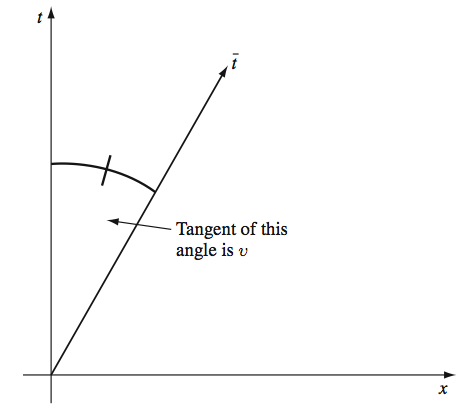
\includegraphics[scale=0.45]{x,t}
\caption{Asse del tempo del riferimento a velocità $v$}
\end{figure}
Possiamo trovare l'asse $\overline{t}$ osservando che rappresenta il luogo degli eventi a $\overline{x}=0$, ovvero il luogo delle coordinate delle coordinate spaziali dell'origine di $\mathcal{O}$. Il risultato è mostrato in Fig. 2.1. L'angolo tra $\overline{t}$ e $t$ possiamo denominarlo con $\psi$, e dunque abbiamo che $v=\tanh\psi$, cioè il coefficiente angolare della retta è $v$. \\
Per trovare l'asse $\overline{x}$, formiamo una costruzione ideata per determinare il luogo degli eventi a $\overline{t}=0$, ovvero quelli che $\mathcal{\overline{O}}$ percepisce come simultanei con $\overline{x}=\overline{t}=0$. L'asse $\overline{x}$ è caratterizzato dalla seguente proprietà: un raggio di luce emesso all'evento $\mathcal{E}$ da $\overline{x}=0$ al tempo $\overline{t}=-a$, raggiungerà l'asse $\overline{x}$ in $\overline{x}=a$ (evento $\mathcal{P}$). Se riflesso, il raggio tornerà in $\overline{x}=0$ al tempo $\overline{t}=a$, che chiameremo evento $\mathcal{R}$. 
\begin{figure}[!h]
\centering
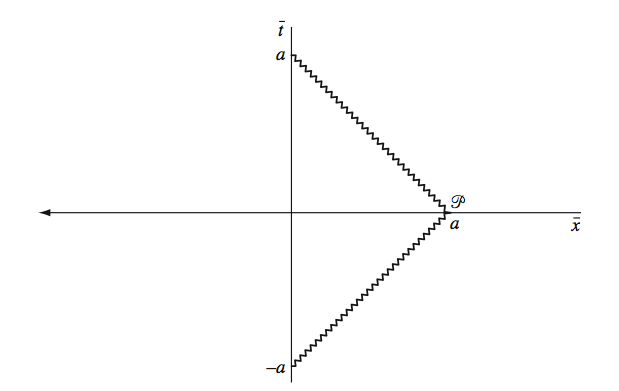
\includegraphics[scale=0.45]{x}
\caption{Luce riflessa}
\end{figure}
Quindi possiamo definire l'asse $\overline{x}$ come il luogo degli eventi che riflettono il raggio di luce in maniera tale che tornerà sull'asse $\overline{t}$ in $+a$ se lo ha lasciato in $-a$. Siccome il procedimento vale per ogni $a$, non è necessaria alcuna assunzione sulla calibrazione di $\overline{t}$ rispetto a $t$, visto che $\mathcal{E}$ è arbitrario.  Quanto dobbiamo fare ora è tracciare lo stesso raggio di luce a partire da $\overline{t}=-a$, ma nel diagramma spaziotemporale $x,t$, che viaggerà a $45^{\circ}$. Dovendo il raggio arrivare in $\mathcal{R}$ sempre con la stessa pendenza di $45^{\circ}$, sarà sufficiente tracciare la perpendicolare a $\overline{t}$ in $\mathcal{R}$ e trovarne l'intersezione con il raggio di luce partito da $\mathcal{E}$: tracciando la retta che congiunge l'intersezione con l'origine avremo l'asse $\overline{x}$. 
\begin{figure}[!h]
\centering
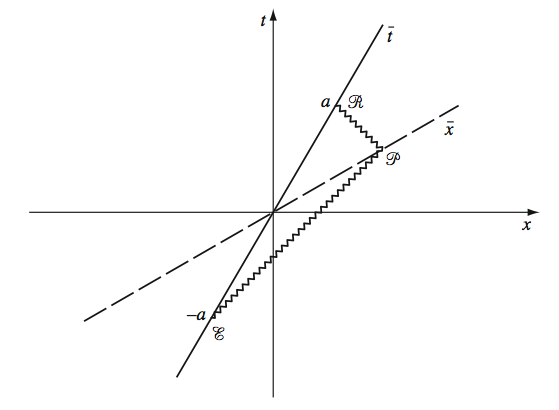
\includegraphics[scale=0.45]{assi}
\caption{Assi $\overline{x}$ e $\overline{t}$}
\end{figure}
Osserviamo che l'asse $\overline{x}$ non coincide con l'asse $x$, per il semplice fatto che la slope di un raggio di luce è sempre $45^{\circ}$ indipendentemente dal sistema di riferimento, mentre $\overline{t}$ modifica la propria pendenza rispetto a $t$. Questa situazione rappresenta l'incarnazione del secondo principio della relatività speciale, ovvero che $c=1$ per ogni sistema di riferimento. Quando applichiamo questo principio alla costruzione geometrica dei sistemi di riferimento ci rendiamo conto che eventi simultanei in $\mathcal{O}$ non lo sono in $\overline{\mathcal{O}}$: questo \emph{fallimento della simultaneità} è inevitabile.    

%\subsection{Invarianza dell'intervallo}
%Consideriamo due eventi $\mathcal{E}$ e $\mathcal{P}$ nel sistema inerziale $\mathcal{O}$, che siano posti sulla linea di universo  dello stesso raggio di luce. Per il semplice fatto che $c=1$ si ha che le differenze  $(\Delta t, \Delta x, \Delta y, \Delta z)$ tra le coordinate di $\mathcal{E}$ e $\mathcal{P}$ in $\mathcal{O}$ soddisfano la relazione 
%\[
%-(\Delta t)^2+ (\Delta x)^2+ (\Delta y)^2+ (\Delta z)^2=0
%\] 
%Per l'universalità della velocità della luce, però, la stessa cosa deve valere anche nelle coordinate di un altro riferimento inerziale $\mathcal{\overline{O}}$, e dunque
%\[
%-(\Delta \overline{t})^2+ (\Delta \overline{x})^2+ (\Delta \overline{y})^2+ (\Delta \overline{z})^2=0
%\]
%Di conseguenza, definiamo l'\textbf{intervallo} tra due eventi (non necessariamente posti sulla linea di universo dello stesso raggio di luce) come:
%\begin{equation}
%\Delta s^2=-(\Delta t)^2+ (\Delta x)^2+ (\Delta y)^2+ (\Delta z)^2
%\end{equation}
%Ne consegue che se $\Delta s^2=0$ in un riferimento inerziale $\mathcal{O}$, necessariamente $\Delta \overline{s}^2=0$ nelle coordinate del sistema $\mathcal{\overline{O}}$. Cosa implica tutto questo per quanto riguarda la relazione tra le coordinate di $\mathcal{O}$ e $\mathcal{\overline{O}}$? Per rispondere a questa domanda, dobbiamo supporre che la relazione tra le coordinate dei due sistemi sia lineare, e che inoltre e due origini coincidano in $t=\overline{t}=0$. Questo significa dunque che i $\Delta \overline{j}$ sono combinazioni lineari dei $\Delta j$, e conseguentemente
%\[
%\Delta \overline{s}^2=-(\Delta \overline{t})^2+ (\Delta \overline{x})^2+ (\Delta \overline{y})^2+ (\Delta \overline{z})^2
%\]
%è una funzione quadratica nelle coordinate non barrate. Possiamo quindi scriverlo come:
%\begin{equation}\label{eq:somma}
%\Delta \overline{s}^2=\sum_{\alpha=0}^3 \sum_{\beta=0}^3 \textbf{M}_{\alpha\beta}\Delta x^{\alpha}\Delta x^{\beta}=\textbf{M}_{\alpha\beta}\Delta x^{\alpha}\Delta x^{\beta}
%\end{equation}
%dove $\textbf{M}_{\alpha\beta}$ posono essere funzioni della velocità relativa $\textbf{v}$. Osserviamo che possiamo supporre $\textbf{M}_{\alpha\beta}=\textbf{M}_{\beta\alpha}$ per ogni $\alpha$ e $\beta$, poichè in (\ref{eq:somma}) conta soltanto la loro somma quando $\alpha\not= \beta$ (lo si può notare svolgendola esplicitamente). Supponiamo ora che $\Delta s^2=0$: ne deduciamo che
%\[
%\Delta r \equiv \Delta t \qquad \Delta r=[(\Delta x)^2+ (\Delta y)^2+ (\Delta z)^2]^{1/2}
%\]
%da cui, sostituendo in (\ref{eq:somma})
%\[
%\Delta \overline{s}^2=\textbf{M}_{00}(\Delta r)^2+2\left( \sum_{i=1}^3 \textbf{M}_{0i}\Delta x^i \right)\Delta r+\sum_{i=1}^3\sum_{j=1}^3 \textbf{M}_{ij}\Delta x^i \Delta x^j
%\]

\subsection{Il cono luce}
Siccome, come abbiamo visto, $\Delta s^2$ è una proprietà dei soli eventi e non dell'osservatore: di conseguenza possiamo utilizzarla per classificare le relazioni tra gli eventi. Se $\Delta s^2>0$, ovvero l'incremento spaziale domina su quello temporale, diremo che i due eventi sono \textbf{spacelike separati}. Nel caso contrario, $\Delta s^2<0$, i due eventi si dicono \textbf{timelike separati}. Infine, se $\Delta s^2=0$ (gli eventi sono, cioè, posti sullo stesso raggio di luce) diremo che gli eventi sono \textbf{lightlike separati}. Gli eventi lightlike separati da un qualsiasi evento $\mathcal{A}$ giacciono su un cono il cui vertice è posto in $\mathcal{A}$. 
\begin{figure}[!h]
\centering
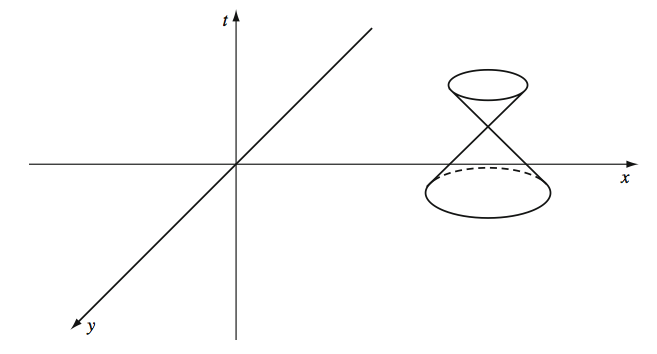
\includegraphics[scale=0.45]{conoluce}
\caption{Il cono luce di un evento (l'asse $z$ è stato omesso)}
\end{figure}
Questo viene chiamato \textbf{cono luce} in $\mathcal{A}$. Tutti gli eventi all'interno del cono luce sono timelike separati da $\mathcal{A}$, mentre quelli al di fuori sono spacelike separati da $\mathcal{A}$ stesso. Siccome nessun oggetto può muoversi ad una velocità superiore a quella della luce, tutte le linee di universo di oggetti fisici si muovono in una direzione timelike. Quindi, un corpo fisico in $\mathcal{A}$ può raggiungere qualsiasi evento all'interno del cono, ma non quelli all'esterno. Per questo motivo gli eventi all'interno del cono luce \emph{futuro} vengono detti \textbf{futuro assoluto} del vertice, mentre quelli all'interno del cono luce \emph{passato} vengono detti \textbf{passato assoluto}. Quelli all'esterno vengono invece detti  \textbf{assolutamente altrove} rispetto ad $\mathcal{A}$. Gli eventi sul cono costituiscono dunque il confine tra il passato ed il futuro assoluti. Quanto è importante notare è che, nonostante in relatività speciale lo spazio ed il tempo possono essere trasformati l'uno nell'altro, è comunque possibile parlare di passato e futuro in una maniera invariante: il cono luce, cioè, definisce un'orientazione temporale. 
\begin{figure}[!h]
\centering
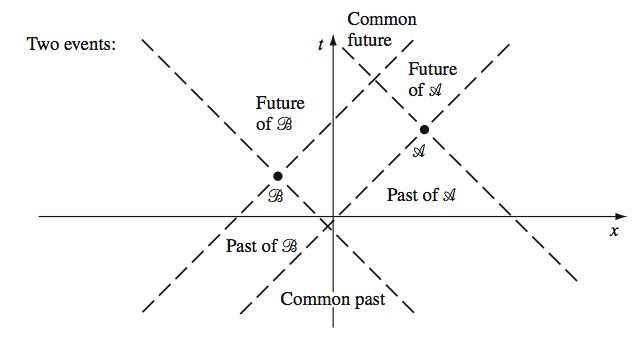
\includegraphics[scale=0.45]{past_future}
\caption{Passato e futuro di due eventi}
\end{figure}
Per Newton e Galileo il passato era rappresentato da qualsiasi cosa avvenuta prima di \emph{adesso}: tutto lo spaziotempo era costituito dall'unione di passato e futuro, il cui unico confine era rappresentato dall'\emph{adesso}. In relatività speciale, invece, il passato è l'insieme degli eventi contenuti nel cono luce passato, ed analogamente per il futuro. In più, tutti gli osservatori concordano su che cosa costituisca il passato ed il futuro e l'altrove di un certo evento. 

\subsection{L'iperbole invariante}
Restringiamoci ora al piano $t-x$, e consideriamo la curva
\[
-t^2+x^2=a^2
\]
 dove $a\in\mathbb{R}$. Questa curva rappresenta un'iperbole nel diagramma spaziotemporale di $\mathcal{O}$, e passa attraverso tutti gli eventi il cui intervallo dall'origine è dato da $a^2$. Dall'invarianza dell'intervallo otteniamo che gli stessi eventi hanno intervallo $a^2$ anche rispetto all'origine di $\mathcal{\overline{O}}$, e dunque giacciono anche sulla curva
 \[
 -\overline{t}^2+\overline{x}^2=a^2
 \]
 Questa è un'iperbole spacelike separata dall'origine. Similmente, gli eventi sulla curva
 \[
 -t^2+x^2=-b^2
 \]
 sono tutti contraddistinti dallo stesso intervallo $-b^2$ dall'origine e giacciono contemporaneamente sulla curva
 \[
  -\overline{t}^2+\overline{x}^2=-b^2
 \]
 Queste iperbole sono asintotiche alle rette con pendenza $\pm 1$, che rappresentano ovviamente i raggi di luce passanti per l'origine. In un diagramma tridimensionale si avrebbe che queste iperboli sono asintotiche al cono luce. 
\begin{figure}[!h]
\centering
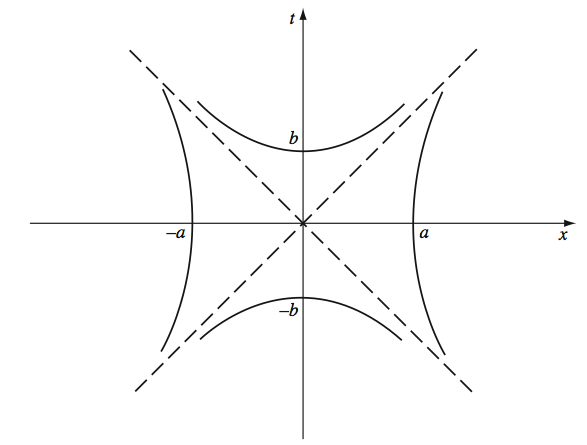
\includegraphics[scale=0.45]{iperbole}
\caption{Iperbole invariante}
\end{figure}
Ora possiamo calibrare gli assi $\overline{t}$ e $\overline{x}$ del riferimento $\mathcal{\overline{O}}$ nel diagramma spaziotemporale di $\mathcal{O}$. Consideriamo ad esempio l'iperbole invariante $-t^2+x^2=-1$. Se consideriamo un evento $\mathcal{A}$ sull'asse temporale, cioè $x=0$, avremo dall'equazione della curva che $t=1$. Similmente, l'evento $\mathcal{B}$ posto sull'asse $\overline{t}$ e dunque $\overline{x}=0$, ha $\overline{t}=1$. Quest'iperbole ci ha dunque permesso di calibrare l'asse temporale. Possiamo fare lo stesso ragionamento con l'iperbole $-t^2+x^2=4$, ad esempio, per calibrare l'asse spaziale. 
\begin{figure}[!h]
\centering
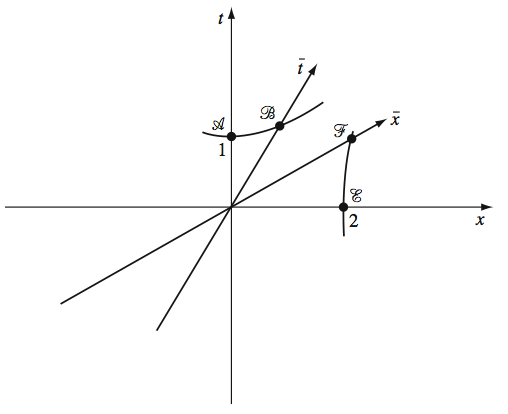
\includegraphics[scale=0.45]{calibrazione}
\caption{Calibrazione degli assi}
\end{figure}
Possiamo subito notare dall'immagine che l'evento $\mathcal{B}$ è più distante di $\mathcal{A}$ dall'origine di $\mathcal{O}$, e questo fatto non fa altro che rimarcare l'inappropriatezza di utilizzare ragionamenti euclidei nell'ambito della relatività ristretta. 
\newpage

\subsection{Addizione delle velocità}
La traiettoria di una particella in moto è descritta in \textbf{F} dalla funzione vettoriale $\textbf{x}(t)$, e in \textbf{F}' da $\textbf{x}'(t')$. Dalle trasformazioni di Lorentz si ricava facilmente che
\begin{equation}\label{eq:addizione}
u'_x = \frac{u_x-v}{1-u_xv/c^2} \quad u'_y=\frac{u_y}{\gamma(1-u_xv/c^2)} \quad u'_z = \frac{u_z}{\gamma(1-u_xv/c^2)}
\end{equation}
Consideriamo ad esempio la prima. E' noto dalle trasformazioni di Lorentz che:
\[
dt' = \gamma \left( dt-\frac{v}{c^2}dx \right)
\]
da cui, raccogliendo $dt$
\[
dt' = \gamma\left( 1-\frac{vu_x}{c^2} \right)dt
\]
con $u_x=dx/dt$. Considerando anche l'altro termine del boost otteniamo:
\[
dx' = \gamma(u_x-v)dt
\]
Dunque, definendo $u'_x\equiv dx'/dt'$
\[
u'_x=\frac{u_x-v}{1-\frac{vu_x}{c^2}}
\]
Le altre due formule si ottengono da ragionamenti esattamente analoghi, tenendo però conto del fatto che $dy'=dy$ e $dz'=dz$. \\
Quanto vogliamo fare ore è ottenere le trasformazioni di Lorentz in forma vettoriale, in modo da ottenere una forma vettoriale anche per la formula dell'addizione delle velocità. Per prima cosa, consideriamo il vettore $\textbf{r}$, che per comodità scomporremo come
\[
\textbf{r}=\textbf{r}_{//}+\textbf{r}_{\perp}
\]
dove $\textbf{r}_{//}$ è la componente di $\textbf{r}$ parallela alla velocità $\textbf{v}$ del sistema di riferimento, mentre $\textbf{r}_{\perp}$ è la componente ad essa perpendicolare. Noto il fatto che solo le componenti pararllele alla velocità risentono di una contrazione, possiamo scrivere il boost di Lorentz come:
\[
\begin{cases}
t' = \gamma \left( t-\frac{\textbf{v}\cdot \textbf{r}}{c^2} \right) \\
\textbf{r}'=\textbf{r}_{\perp}+\gamma(\textbf{r}_{//}-\textbf{v}t)
\end{cases}
\]
Evidentemente
\[
\textbf{r}_{//}=\frac{\textbf{r}\cdot \textbf{v}}{v^2}\textbf{v}
\]
e di conseguenza
\[
\textbf{r}_{\perp}=\textbf{r}-\frac{\textbf{r}\cdot \textbf{v}}{v^2}\textbf{v}
\]
Quindi:
\[
\textbf{r}'=\textbf{r}-\frac{\textbf{r}\cdot \textbf{v}}{v^2}\textbf{v}+\gamma \left( \frac{\textbf{r}\cdot \textbf{v}}{v^2}\textbf{v}-\textbf{v}t \right)
\]
cioè
\[
\textbf{r}'=\textbf{r}+\left( \frac{\gamma-1}{v^2}(\textbf{r}\cdot\textbf{v})-\gamma t \right)\textbf{v}
\]
La formula vettoriale per l'addizione delle velocità di ottiene quindi considerando il ''boost infinitesimo'':
\[
\begin{cases}
dt' = \gamma \left( dt-\frac{\textbf{v}\cdot d\textbf{r}}{c^2} \right) \\
d\textbf{r}'=d\textbf{r}+\left( \frac{\gamma-1}{v^2}(d\textbf{r}\cdot\textbf{v})-\gamma dt \right)\textbf{v}
\end{cases}
\]
e calcolandone il rapporto, ottenendo:
\[
\textbf{u}'=\frac{d\textbf{r}'}{dt'}=\frac{\textbf{u}+\frac{\gamma-1}{v^2}(\textbf{u}\cdot\textbf{v})\textbf{v}-\gamma\textbf{v}}{\gamma \left( 1-\frac{\textbf{v}\cdot \textbf{u}}{c^2} \right)}
\]
Per un mezzo trasparente in quiete in \textbf{F}' con indice di rifrazione $n$, è noto che la velocità di propagazione della luce nel mezzo stesso è data da
\[
u'=\frac{c}{n}
\]
Di conseguenza, supponendo che il dielettrico si muova parallelamente alla direzione del raggio di luce, possiamo scrivere la formula di addizione delle velocità, per conoscere la v elocità di propagazione della radiazione nel sistema di laboratorio, per come segue, a partire dalla (\ref{eq:addizione}):
\begin{align*}
u&=\frac{u'+v}{1+\frac{vu'}{c^2}}=\frac{\frac{c}{n}+v}{1+\frac{v}{nc}}=\left( \frac{c}{n}+v \right)\left( 1-\frac{v}{nc}+o\left(\frac{v}{n}\right) \right) \\
&=\frac{c}{n}-\frac{v}{n^2}+v+o(v^2) \simeq \frac{c}{n} +v\left( 1-\frac{1}{n^2} \right)
\end{align*}
e viene ripristinata la formula di Fizeau. 
\subsection{Effetto Doppler relativistico}
Usando le formule di trasformazione di Lorentz e la costanza di c nella condizione di invarianza della fase di un onda elettromagnetica piana, si trovano le formule di trasformazione delle caratteristiche dell'onda valide nella teoria della relatività. Scriviamo dunquela fase di un onda elettromagnetica generica
\[
F=\nu \left( t-\frac{x\cos\alpha+y\sin\alpha}{c} \right)
\]
\[
F'=\nu' \left( t'-\frac{x'\cos\alpha'+y'\sin\alpha'}{c} \right)
\]
cioè
\[
F=\nu\gamma \left( t'+\frac{v}{c^2}x' \right)-\frac{\nu\gamma(x'-vt')\cos\alpha+\nu y'\sin\alpha}{c}
\]
Di conseguenza
\[
\nu' t'=\nu\gamma t' -\gamma \nu t' \frac{v}{c}\cos\alpha 
\]
\begin{equation}\label{eq:nu}
 \nu' = \nu \gamma \left( 1-\frac{v}{c}\cos\alpha \right)
\end{equation}
Inoltre
\[
-\nu'\frac{x'}{c}\cos\alpha' = \nu \gamma\frac{v}{c^2}x'-\nu\gamma \frac{x'}{c}\cos\alpha
\]
da cui
\begin{equation}\label{eq:nucos}
\nu'\cos\alpha' = \nu\gamma \left(\cos\alpha-\frac{v}{c} \right)
\end{equation} 
Dalla (\ref{eq:nu}) e (\ref{eq:nucos}) e osservando che
\begin{equation}\label{eq:sin}
\nu'\sin\alpha' = \nu\sin\alpha
\end{equation}
otteniamo che
\begin{equation}\label{eq:nutan}
\tan\alpha' = \frac{\sin\alpha}{\gamma \left( \cos\alpha-\frac{v}{c} \right)}
\end{equation}
L'effetto Doppler è contenuto nelle relazioni (\ref{eq:nu}), (\ref{eq:nucos}) e (\ref{eq:sin}): se la sorgente è in \textbf{F}', allora $\alpha$ è l'angolo tra la direzione del moto della sorgente e la direzione della luce in \textbf{F}. Inoltre $v_r = -v\cos\alpha$, dove $v_r$ è considerata positiva se la sorgente si allontana dall'osservatore. Si ottiene allora la formula relativistica
\begin{equation}
\nu = \frac{\nu'}{\gamma(1+v_r/c)}
\end{equation}
Si noti che secondo questa formula c'è effetto Doppler anche per $v_r=0$, ossia per un puro moto trasverso. \\
L'aberrazione, invece, è contenuta nella (\ref{eq:nutan}), valida per ogni coppia di riferimenti inerziali. In particolare, se \textbf{F} è il sistema di quiete della sorgente e \textbf{F}' rappresenta un laboratorio terrestre nel suo moto attorno al Sole, la direzione del raggio in \textbf{F} è $\vartheta=\pi-\alpha$, in \textbf{F}' è $\vartheta'=\pi-\alpha'$, e si ottiene dunque:
\[
\tan\vartheta' = \frac{\sin\vartheta}{\gamma \left( \cos\vartheta+\frac{v}{c} \right)}
\]
\subsection{Onde di materia}
da aggiungere (nuove dispense Vanzo)
\chapter{Analisi tensoriale in relatività speciale}
\section{Vettori}
Rivediamo in questa sezione alcune nozioni di algebra vettoriale, anche con il solo semplice scopo di concordare sulla nuova notazione che verrà utilizzata. 

\subsection{Notazione}
Denoteremo i vettori con $\textbf{x}$ e indicheremo con
\[
\Delta\textbf{x}\underset{\mathcal{O}}{\to} \{\Delta x^{\alpha} \}
\]
le sue componenti nel sistema di riferimento $\mathcal{O}$, per $\alpha\in\{0,1,2,3\}$. Se volessimo riscrivere il vettore $\Delta \textbf{x}$ in un altro sistema di riferimento, ad esempio $\overline{\mathcal{O}}$, scriveremmo
\[
\Delta \textbf{x} \underset{\mathcal{\overline{O}}}{\to} \{ \Delta x^{\overline{\alpha}} \}
\]
cioè \emph{barriamo} l'indice per denotare le nuove coordinate. Ovviamo il vettore è \emph{lo stesso}, sono solo le sue componenti a cambiare. Le nuove componenti le otterremo attraverso una trasformazione di Lorentz che, essendo lineare, scriveremo come
\begin{equation}\label{eq:vec1}
\Delta x'^{\overline{\alpha}} = \Lambda _{\beta}^{\overline{\alpha}}\Delta x^{\beta}
\end{equation}
dove abbiamo, come al solito (ed oramai eviteremo di specificarlo) utilizzato la notazione di Einstein sulla somma di indici ripetuti. Osserviamo preventivamente che
\[
\Delta x'^{\overline{\alpha}} = \Lambda _{\gamma}^{\overline{\alpha}}\Delta x^{\gamma}
\]
in quanto $\beta$ e $\gamma$ giocano il ruolo di \textbf{indici muti}, e dunque possono essere sotituiti da altri indici muti in maniera arbitraria. Al contrario, gli indici come $\overline{\alpha}$, su cui non è calcolata alcuna somma, vengono detti \textbf{indici liberi}: ovviamente, il nome assegnato ad un indice libero è assolutamente arbitrario.

\subsection{Trasformazione di basi}
Fissata una base $\{ \textbf{e}_{\alpha} \}$, possiamo sempre esprimere un vettore come
\[
\textbf{A} = A^{\alpha} \textbf{e}_{\alpha}
\]
Questo è vero per qualunque sistema di riferimento e dunque è altrettanto corretto scrivere
\[
\textbf{A} = A^{\overline{\alpha}} \textbf{e}_{\overline{\alpha}}
\]
Utilizzando (\ref{eq:vec1}) possiamo riscrivere quest'ultima uguaglianza come
\[
\Lambda _{\beta}^{\overline{\alpha}}A^{\beta}\textbf{e}_{\overline{\alpha}} = A^{\alpha}\textbf{e}_{\alpha}
\]
Sulla sinistra abbiamo due somme, che essendo finite non tengono conto dell'ordine in cui sono calcolate. Di conseguenza:
\[
A^{\beta}\Lambda _{\beta}^{\overline{\alpha}}\textbf{e}_{\overline{\alpha}} = A^{\alpha}\textbf{e}_{\alpha}
\]
Ora, tenendo conto del fatto che $\beta$ e $\overline{\alpha}$ sono indici muti, scriviamo $\beta \equiv \alpha$ e $\overline{\alpha} \equiv \overline{\beta}$:
\[
A^{\alpha}\Lambda _{\alpha}^{\overline{\beta}}\textbf{e}_{\overline{\beta}} = A^{\alpha}\textbf{e}_{\alpha}
\]
Dal fatto che $\textbf{A}$ è un vettore arbitrario, l'equazione precedente deve essere vera per ogni set $\{ A^{\alpha} \}$. Scriviamola allora come:
\[
A^{\alpha} (  \Lambda _{\alpha}^{\overline{\beta}}\textbf{e}_{\overline{\beta}} -\textbf{e}_{\alpha}) =0
\]
da cui
\begin{equation}\label{eq:vec2}
\textbf{e}^{\alpha} = \Lambda _{\alpha}^{\overline{\beta}}\textbf{e}_{\overline{\beta}}
\end{equation}
che è la formula di trasformazione dei vettori di una base. 

\subsection{Trasformazione inversa}
Sappiamo che il boost di Lorentz dipende solo dalla velocità relativa dei due riferimenti: esplicitiamolo scrivendo
\[
\Lambda_{\alpha}^{\overline{\beta}}=\Lambda_{\alpha}^{\overline{\beta}}(\textbf{v})
\]
Quindi, dalla (\ref{eq:vec2}) abbiamo
\[
\textbf{e}^{\alpha} = \Lambda _{\alpha}^{\overline{\beta}}(\textbf{v})\textbf{e}_{\overline{\beta}}
\]
Ora ci rendiamo conto del fatto che se $\textbf{v}$ è la velocità del riferimento $\overline{\mathcal{O}}$ rispetto a $\mathcal{O}$, allora la velocità di $\mathcal{O}$ rispetto a $\overline{\mathcal{O}}$ sarà $-\textbf{v}$. Di conseguenza possiamo scrivere
\[
\textbf{e}_{\overline{\beta}}=\Lambda_{\overline{\beta}}^{\nu}(-\textbf{v})\textbf{e}_{\nu}
\]
Chiaramente $\Lambda_{\overline{\beta}}^{\nu}$ e $\Lambda _{\alpha}^{\overline{\beta}}$ sono la stessa matrice, con la semplice differenza che $\textbf{v} \to -\textbf{v}$. Ora possiamo scrivere:
\[
\textbf{e}^{\alpha} = \Lambda _{\alpha}^{\overline{\beta}}(\textbf{v})\textbf{e}_{\overline{\beta}} = \Lambda _{\alpha}^{\overline{\beta}}(\textbf{v})\Lambda_{\overline{\beta}}^{\nu}(-\textbf{v})\textbf{e}_{\nu}
\]
che deriva dalle precedenti relazioni che abbiamo trovato. A questo punto vi sono due somme: una su $\overline{\beta}$ e una su $\nu$. Immaginando di sommare prima su $\overline{\beta}$, si avrebbe che $\textbf{e}_{\alpha}$ è combinazione lineare dei  vettori della base $\{ \textbf{e}_{\nu}\}$ con coefficienti
\[
\sum_{\overline{\beta}}\Lambda _{\alpha}^{\overline{\beta}}(\textbf{v})\Lambda_{\overline{\beta}}^{\nu}(-\textbf{v})
\]
Allora, fissando l'indice $\alpha$ deve essere per forza vero che
\begin{equation}\label{eq:vec3}
\Lambda _{\alpha}^{\overline{\beta}}(\textbf{v})\Lambda_{\overline{\beta}}^{\nu}(-\textbf{v})=\delta_{\alpha}^{\nu}
\end{equation}
cioè $\Lambda_{\overline{\beta}}^{\nu}(-\textbf{v})$ è la matrice inversa di $\Lambda _{\alpha}^{\overline{\beta}}(\textbf{v})$. 

\section{Tensori $\binom{0}{N}$}
Diamo la seguente definizione di tensore:
\begin{defn}
Sia $V$ uno spazio vettoriale sul campo $\mathbb{R}$. Un\textbf{ tensore di tipo $\binom{0}{N}$} è una forma N-lineare 
\[
\begin{matrix} T:\underbrace{ V\times V \times \ldots \times V }_{N-volte} \to \mathbb{R}\end{matrix} 
\]
\end{defn}
Un esempio di tensore di tipo $\binom{0}{N}$ per $N=2$ è il prodotto scalare. Infatti, sia $V$ uno spazio vettoriale: l'applicazione $\cdot : V\times V\to\mathbb{R}$ che mappa $(\textbf{A},\textbf{B})\mapsto \textbf{A}\cdot \textbf{B}$ è certamente bilineare. Per dare concretezza al fatto che il prodotto scalare rappresenta un tensore, definiamo il \textbf{tensore metrico} $\textbf{g}$ come quel tensore tale che
\[
\textbf{g}(\textbf{A},\textbf{B}) := \textbf{A}\cdot \textbf{B}
\]
Osserviamo subito che la definizione di tensore non riguarda in alcun modo le componenti dei vettori su cui viene applicato: infatti è necessario che un tensore risulti essere un concetto sufficientemente generale da non dipendere dalla base scelta sullo spazio vettoriale. 

\begin{defn}
Le \textbf{componenti sul riferimento $\mathcal{O}$ di un tensore $T$ di tipo $\binom{0}{N}$} sono le immagini rispetto a $T$ dei vettori della base $\{ \textbf{e}_{\alpha} \}$ di $V$ che rappresenta $\mathcal{O}$. 
\end{defn}
Questo significa che le componenti di un tensore dipendono dalla base che scegliamo per rappresentare lo spazio vettoriale. Le componenti del tensore metrico sono date da:
\[
\textbf{g}(\textbf{e}_{\alpha},\textbf{e}_{\beta})=\textbf{e}_{\alpha}\cdot \textbf{e}_{\beta}=\eta_{\alpha\beta}
\]
dove $\eta_{\alpha\beta}$ è la matrice che già in precedenza abbiamo introdotto. 

\subsection{I tensori $\binom{0}{1}$: le 1-forme}
Il caso $\binom{0}{1}$ è molto semplice da trattare. Infatti i tensori di questo tipo non sono altro che applicazioni lineari $T\in\Hom(V,\mathbb{R})\equiv V^*$, cioè elementi dello \textbf{spazio duale} a $V$. Quanto vogliamo fare ora è indagare alcune proprietà generali della 1-forme: per farlo, la generica 1-forma verrà sempre indicata con $\tilde{p}$. 
\\
Le componenti di una 1-forma verranno denotate con $p_{\alpha}$:
\[
p_{\alpha}:= \tilde{p}(\textbf{e}_{\alpha})
\]
al contrario delle componenti di un vettore, che vengono convenzionalmente indicate con l'indice in alto. In termini della componenti, possiamo scrivere:
\begin{equation}\label{eq:1form1}
\tilde{p}(\textbf{A})=\tilde{p}(A^{\alpha}\textbf{e}_{\alpha})=A^{\alpha}\tilde{p}(\textbf{e}_{\alpha})=A^{\alpha}p_{\alpha}
\end{equation}
operazione detta \textbf{contrazione} di $\textbf{A}$ e $\tilde{p}$. Le componenti di $\tilde{p}$ sulla base $\{ \textbf{e}_{\overline{\beta}} \}$ sono date invece da:
\[
p_{\overline{\beta}}:=\tilde{p}(\textbf{e}_{\overline{\beta}})=\tilde{p}(\Lambda_{\overline{\beta}}^{\alpha}\textbf{e}_{\alpha}) = \Lambda_{\overline{\beta}}^{\alpha}\tilde{p}(\textbf{e}_{\alpha})=\Lambda_{\overline{\beta}}^{\alpha}p_{\alpha}
\]
Questo significa che le 1-forme trasformano esattamente come i vettori di una base e in maniera opposta alle componenti dei vettori (cioè utilizzano la matrice inversa). \\
Osserviamo ora che $A^{\alpha}p_{\alpha}$ è indipendente dal sistema di riferimento. Infatti:
\begin{align*}
A^{\overline{\alpha}}p_{\overline{\alpha}}=(\Lambda_{\beta}^{\overline{\alpha}} A^{\beta})(\Lambda_{\overline{\alpha}}^{\mu}p_{\mu})= \Lambda_{\beta}^{\overline{\alpha}}\Lambda_{\overline{\alpha}}^{\mu} A^{\beta}p_{\mu}= \delta _{\beta}^{\mu}A^{\beta}p_{\mu} = A^{\beta}p_{\beta}
\end{align*}
Vogliamo ora costruire una base per lo spazio duale, cioè trovare un set $\{ \tilde{w}^{\alpha} \}$ di 1-forme linearmente indipendenti tale che:
\[
\tilde{p}=p_{\alpha}\tilde{w}^{\alpha}
\]
Sappiamo inoltre dalla (\ref{eq:1form1}) che 
\[
\tilde{p}(\textbf{A})=p_{\alpha}A^{\alpha}
\]
e dunque
\[
p_{\alpha}A^{\alpha}= \tilde{p}(\textbf{A}) = p_{\alpha}\tilde{w}^{\alpha}(\textbf{A})=p_{\alpha}\tilde{w}^{\alpha}(A^{\beta}\textbf{e}_{\beta})=p_{\alpha}A^{\beta}\tilde{w}^{\alpha}(\textbf{e}_{\beta})
\]
da cui
\[
p_{\alpha}A^{\alpha} = p_{\alpha}A^{\beta}\tilde{w}^{\alpha}(\textbf{e}_{\beta}) \text{ } \forall \alpha,\beta \Longleftrightarrow \tilde{w}^{\alpha}(\textbf{e}_{\beta})=\delta_{\beta}^{\alpha}
\]
Quindi
\begin{equation}\label{eq:1form2}
\tilde{w}^{\alpha}(\textbf{e}_{\beta})=\delta_{\beta}^{\alpha}
\end{equation}
La relazione (\ref{eq:1form2}) \emph{definisce} gli elementi di una base dello spazio duale, poichè è valida $\forall \alpha$. Ora rimane da determinare solo come $\{ \tilde{w}^{\alpha}\}$ si modifichi per cambi di base. La trattazione è completamente analoga a quella per i vettori, e conduce, come atteso, alla relazione
\begin{equation}
\tilde{w}^{\overline{\alpha}}=\Lambda_{\beta}^{\overline{\alpha}}\tilde{w}^{\beta}
\end{equation}
\subsection{I tensori $\binom{0}{2}$}
Possiamo introdurre i tensori di tipo $\binom{0}{2}$ attraverso un opportuno prodotto, cioè prese due 1-forme $\tilde{p}$ e $\tilde{q}$ definiamo
\[
\tilde{p}(\textbf{A})\tilde{q}(\textbf{B}) =: \textbf{f}(\textbf{A},\textbf{B})
\]
detto \textbf{prodotto tensoriale di 1-forme}, e indicato con $\textbf{f}=\tilde{p}\otimes \tilde{q}$. Tale prodotto è ovviamente non commutativo, infatti
\[
\tilde{p}\otimes\tilde{q}(\textbf{A},\textbf{B}) = \tilde{p}(\textbf{A})\tilde{q}(\textbf{B}) \not= \tilde{q}(\textbf{A})\tilde{p}(\textbf{B})=\tilde{q}\otimes\tilde{p}(\textbf{A},\textbf{B})
\]
Vediamo però come ottenere una forma generale di un tensore di tipo $\binom{0}{2}$ pensandolo come combinazione lineare degli elementi di una base. Sappiamo che le componenti di un tensore $\textbf{f}$ saranno dati da
\[
f_{\alpha\beta} := \textbf{f}(\textbf{e}_{\alpha},\textbf{e}_{\beta})
\]
Dato il fatto che ciascuno dei due indici può assumere 4 valori, il tensore sarà contraddistinto da 16 componenti. Il valore di $\textbf{f}$ su una coppia arbitraria di vettori è dato da:
\[
\textbf{f}(\textbf{A},\textbf{B}) = \textbf{f}(A^{\alpha}\textbf{e}_{\alpha},B^{\beta}\textbf{e}_{\beta})=A^{\alpha}B^{\beta}f_{\alpha\beta}
\]
Ora indaghiamo come sia possibile trovare un set di 16 tensori $\tilde{w}^{\alpha\beta}$ in modo tale che
\[
\textbf{f}=f_{\alpha\beta}\tilde{w}^{\alpha\beta}
\]
In questo caso avremmo
\[
f_{\mu\nu}=\textbf{f}(\textbf{e}_{\mu},\textbf{e}_{\nu})=f_{\alpha\beta}\tilde{w}^{\alpha\beta}(\textbf{e}_{\mu},\textbf{e}_{\nu})
\]
da cui, come prima, otteniamo che
\[
\tilde{w}^{\alpha\beta}(\textbf{e}_{\mu},\textbf{e}_{\nu})=\delta^{\alpha}_{\mu}\delta^{\beta}_{\nu}
\]
Sappiamo però che $\delta^{\alpha}_{\mu}=\tilde{w}^{\alpha}(\textbf{e}_{\mu})$ e $\delta^{\beta}_{\nu}=\tilde{w}^{\beta}(\textbf{e}_{\nu})$ e di conseguenza
\begin{equation}\label{eq:2form1}
\tilde{w}^{\alpha\beta}=\tilde{w}^{\alpha}\otimes \tilde{w}^{\beta}
\end{equation}
da cui
\begin{equation}\label{eq:2form2}
\textbf{f}=f_{\alpha\beta}\tilde{w}^{\alpha}\otimes \tilde{w}^{\beta}
\end{equation}
E' evidente notare che il valore di un tensore dipende dall'ordine dei suoi argomenti: il comportamento di un tensore sotto lo scambio degli argomenti è una proprietà fondamentale che lo contraddistingue. Diremo che un tensore è \textbf{simmetrico} se 
\[
\textbf{f}(\textbf{A},\textbf{B}) = \textbf{f}(\textbf{B},\textbf{A}) \text{ } \forall \textbf{A},\textbf{B}
\]
mentre è \textbf{antisimmetrico} quando
\[
\textbf{f}(\textbf{A},\textbf{B}) = -\textbf{f}(\textbf{B},\textbf{A}) \text{ } \forall \textbf{A},\textbf{B}
\]
Questo deve valere in particolare per i vettori di una base, e di conseguenza, posto $\textbf{A}=\textbf{e}_{\alpha}$ e $\textbf{B}=\textbf{e}_{\beta}$ otteniamo che
\[
f_{\alpha\beta}=f_{\beta\alpha}
\]
per un tensore simmetrico, mentre
\[
f_{\alpha\beta}=-f_{\beta\alpha}
\]
per un tensore antisimmetrico. Dato un qualunque tensore $\textbf{h}$ è sempre possibile costruirne uno simmetrico ed un antisimmetrico a partire da $\textbf{h}$ stesso. Infatti, dal punto di vista delle componenti
\[
h_{(\alpha\beta)}:=\frac{1}{2}(h_{\alpha\beta}+h_{\beta\alpha})
\]
è simmetrico, mentre
\[
h_{[\alpha\beta]}:=\frac{1}{2}(h_{\alpha\beta}-h_{\beta\alpha})
\]
è antisimmetrico. \\
\\
Vogliamo mostrare come si trasformino, in generale, le componenti di un tensore $\binom{0}{2}$. Sia allora 
\[
\textbf{f} = f_{\mu\nu}\tilde{w}^{\mu}\otimes \tilde{w}^{\nu}
\]
un generico tensore $\binom{0}{2}$ (che nel seguito, parlando di relatività, chiameremo \emph{di rango 2}). Possiamo facilmente ricavare la legge di trasformazione per gli elementi di una base. Infatti, dalla legge di trasformazione per le 1-forme
\[
\tilde{w}^{\overline{\alpha}} = \Lambda_{\mu}^{\overline{\alpha}}\tilde{w}^{\mu} \Longrightarrow \Lambda_{\overline{\alpha}}^{\mu}\tilde{w}^{\overline{\alpha}} = \Lambda_{\mu}^{\overline{\alpha}}\Lambda_{\overline{\alpha}}^{\mu}\tilde{w}^{\mu} = \tilde{w}^{\mu}
\]
cioè 
\[
\Lambda_{\overline{\alpha}}^{\mu}\tilde{w}^{\overline{\alpha}} = \tilde{w}^{\mu}
\]
Di conseguenza
\[
\textbf{f} = f_{\mu\nu} ( \Lambda_{\overline{\alpha}}^{\mu}\tilde{w}^{\overline{\alpha}} \otimes \Lambda_{\overline{\beta}}^{\nu}\tilde{w}^{\overline{\beta}}) = \Lambda_{\overline{\alpha}}^{\mu}\,\Lambda_{\overline{\beta}}^{\nu} f_{\mu\nu} \tilde{w}^{\overline{\alpha}} \otimes \tilde{w}^{\overline{\beta}}
\]
Cioè la legge di trasformazione per le componenti di un tensore covariante di rango 2 è data da:
\begin{equation}\label{eq:covariant}
f_{\overline{\alpha}\overline{\beta}} = \Lambda_{\overline{\alpha}}^{\mu}\,\Lambda_{\overline{\beta}}^{\nu} f_{\mu\nu}
\end{equation}

\subsection{Metrica come mappa tra vettori e 1-forme}
Consideriamo $\textbf{g}$ ed un vettore $\textbf{V}$. Possiamo osservare che
\[
\textbf{g}(\textbf{V},\cdot):V\to \mathbb{R}
\]
è un'applicazione lineare tra uno spazio vettoriale ed $\mathbb{R}$, cioè una 1-forma. Denotiamo
\[
\tilde{V} := \textbf{g}(\textbf{V},\cdot) = \textbf{g}(\cdot,\textbf{V})
\]
Ovviamente
\[
\tilde{V}(\textbf{A})=\textbf{g}(\textbf{V},\textbf{A})=\textbf{V}\cdot \textbf{A}
\]
Come sono fatte le componenti di $\tilde{V}$? Esse sono:
\[
V_{\alpha}:=\tilde{V}(\textbf{e}_{\alpha})=\textbf{V}\cdot \textbf{e}_{\alpha}=\textbf{e}_{\alpha}\cdot \textbf{V}=\textbf{e}_{\alpha}\cdot (V^{\beta}\textbf{e}_{\beta})=(\textbf{e}_{\alpha}\cdot \textbf{e}_{\beta})V^{\beta}
\]
cioè
\begin{equation}
V_{\alpha}=\eta_{\alpha\beta}V^{\beta}
\end{equation}
cioè la metrica lega le componenti dei vettori a quelle delle 1-forme. In particolare, con la metrica di Minkowsky della relatività ristretta, la corrispondenza è piuttosto facile, in quanto se $\textbf{V}=(a,b,c,d)$, allora $\tilde{V}=(-a,b,c,d)$. Quest'ultima affermazione è chiaramente non vera nel caso di metriche più complesse. 
\\
Ci chiediamo ora: la metrica ci fornisce anche un modo per per mappare 1-forme in vettori? La risposta è sì: se la matrice $\eta_{\alpha\beta}$ ammette un'inversa allora possiamo trovare le componenti $V^{\beta}$ a partire da $V_{\alpha}$. La matrice inversa esiste grazie al fatto che $\det\eta_{\alpha\beta}=-1\not=0$: la denoteremo con $\eta^{\alpha\beta}$. Dunque:
\begin{equation}
A^{\alpha} = \eta_{\alpha\beta}A_{\alpha}
\end{equation}
\section{Tensori $\binom{M}{N}$}
Nonostante abbiamo definito le 1-forme come funzioni di vettori, possiamo ora notare come i vettori stessi possano essere trattai come applicazioni lineari che mappano 1-forme nei reali. Infatti, dati un vettore $\textbf{V}$ ed una 1-forma $\tilde{p}$ si ha che
\[
\textbf{V}(\tilde{p}) \equiv \tilde{p}(\textbf{V}) \equiv p_{\alpha}V^{\alpha} \equiv \langle \tilde{p},\textbf{V} \rangle
\]
In questo modo evitiamo di trattare i vettori come speciali oggetti su cui i tensori \emph{agiscono}, ma anzi concediamo ad essi stessi il ruolo di tensori. 
\\
Prima di passare alla definizione generale di tensori di tipo $\binom{M}{N}$, definiamo quelli di tipo $\binom{M}{0}$. 
\begin{defn}
Sia $V$ uno spazio vettoriale sul campo $\mathbb{R}$ e sia $V^*$ il suo spazio duale. Un \textbf{tensore di tipo $\binom{M}{0}$} è allora un'applicazione M-zlineare
\[
\begin{matrix} T^*:\underbrace{ V^*\times V^* \times \ldots \times V^* }_{M-volte} \to \mathbb{R}\end{matrix} 
\]
\end{defn}
Tutte le discussioni fatte sui tensori di tipo $\binom{0}{N}$ si applicano anche a questo caso. Un semplice tensore $\binom{2}{0}$ è ottenuto come $\textbf{V}\otimes\textbf{W}$, definito mediante
\[
\textbf{V}\otimes\textbf{W}(\tilde{p},\tilde{q}) := \textbf{V}(\tilde{p})\textbf{W}(\tilde{q}) := \tilde{p}(\textbf{V})\tilde{q}(\textbf{W}) = V^{\alpha}p_{\alpha}W^{\beta}q_{\beta}
\]
Passiamo a questo punto alla generalizzazione del concetto di tensore. 
\begin{defn}
Sia $V$ uno spazio vettoriale sul campo $\mathbb{R}$ e sia $V^*$ il suo spazio duale. Un \textbf{tensore di tipo $\binom{M}{N}$} è un'applicazione multilineare
\[
\begin{matrix} T:\underbrace{V\times V\times \ldots \times V}_{N-volte}\times\underbrace{ V^*\times V^* \times \ldots \times V^* }_{M-volte} \to \mathbb{R}\end{matrix}
\]
Conseguentemente un tensore associa ad N vettori $\textbf{A},...,\textbf{N}$ ed M 1-forme $\tilde{a},...,\tilde{m}$ uno scalare
\[
(\textbf{A},\ldots,\textbf{N};\tilde{a},\ldots,\tilde{m})\mapsto T(\textbf{A},\ldots,\textbf{N};\tilde{a},\ldots,\tilde{m}) \in \mathbb{R}
\]
\end{defn}
Consideriamo ad esempio un tensore $\textbf{R}$ di tipo $\binom{1}{1}$: perchè questo restituisca un numero reale deve essere applicato ad un vettore ed un'1-forma: $\textbf{R}(\textbf{A};\tilde{p})$. Per quanto riguarda le sue componenti:
\[
\textbf{R}(\tilde{w}_{\alpha};\textbf{e}_{\beta}) := \textbf{R}_{\beta}^{\alpha}
\]
Di conseguenza, un tensore generico $\textbf{T}$ di tipo $\binom{M}{N}$ ha componenti:
\[
\textbf{T}(\tilde{w}_{\alpha_1},\ldots,\tilde{w}_{\alpha_M}; \textbf{e}^{\beta_1},\ldots \textbf{e}^{\beta_N}):=\textbf{T}_{\alpha_1,\ldots,\alpha_M}^{\beta_1,\ldots,\beta_N}
\]

\subsection{Innalzamento, abbassamento di indici e contrazione}
Così come i vettori vengono mappati in 1-forme, in una maniera più generale la metrica rappresenta una mappa tensori $\binom{N}{M}\mapsto \binom{N-1}{M+1}$. Similmente, la sua inversa $\binom{N}{M} \mapsto \binom{N+1}{M-1}$. Vediamo un esempio: consideriamo il tensore (facciamo corrispondere, con un abuso di linguaggio, il tensore con le sue componenti) di tipo $\binom{1}{2}$ $T^{\alpha\beta}_{\gamma}$. Osserviamo che:
\[
T^{\alpha}_{\beta\gamma} := \eta_{\beta\mu} T^{\alpha\mu}_{\gamma}
\]
è un tensore di tipo $\binom{1}{2}$, ottenuto \textbf{abbassando un indice}, ovvero mappando il vettore corrispondente nel suo spazio duale. Possiamo anche \textbf{alzare un indice}, mediante la metrica inversa, ottenendo in questo caso un tensore di tipo $\binom{3}{0}$:
\[
T^{\alpha\beta\gamma} := \eta^{\mu\gamma} T^{\alpha\beta}_{\mu}
\]
\\-
La \textbf{contrazione} (o \textbf{contrazione di tensori}) è un'operazione tra due o più tensori che emerge dal pairing tra uno spazio vettoriale ed il suo duale. Definiamo:
\begin{defn}
Sia $V$ uno spazio vettoriale sul campo $\mathbb{K}$ e sia $V^*$ il suo duale. Il \textbf{pairing} di $V$ nel suo duale è la forma bilineare
\[
t: V \times V^* \to \mathbb{K}
\]
definita mediante $t( \textbf{v}, \tilde{w} ) := \tilde{w}(\textbf{v})$. 
\end{defn}
Il pairing dunque rappresenta la contrazione tra tensori di tipo $\binom{1}{1}$, ma chiaramente possiamo estenderla a tensori di tipo $\binom{M}{N}$. Consideriamo infatti la mappa che applichi il pairing al $k$-esimo vettore e alla $l$-esima 1-forma e l'identità a tutti gli altri vettori: questa operazione definisce la contrazione delle componenti $(k,l)$, e dunque funge da mappa $\binom{M}{N} \mapsto \binom{M-1}{N-1}$. Per un tensore di rango 2 la contrazione viene detta \textbf{traccia}:
\[
K^a_a = \eta^{ab}K_{ab} = \eta_{ab}K^{ab}
\]
Possiamo verificare che il risultato di tale contrazione è un invariante di Lorentz. Infatti, consideriamo un tensore di tipo $\binom{1}{1}$
\[
\textbf{T} = a_{ij} \textbf{e}_{i} \otimes \tilde{e}^{j}
\]
Ovviamente 
\[ t(\textbf{T})=a_{ij}t(\textbf{e}^{i} \otimes \tilde{e}_{j}) = a_{ij}\tilde{e}_{j}(\textbf{e}^i)=\delta^i_j a_{ij} \]
cioè la contrazione corrisponde effettivamente al calcolo della traccia della matrice dei coefficienti del tensore, che è notoriamente invariante per cambio di base. 
\chapter{Equazioni invarianti}
\section{Struttura del gruppo di Lorentz}
Come abbiamo già discusso, il gruppo delle trasformazioni di Lorentz 
\[
x^a \to x^a = \Lambda_a^b x^b 
\]
è quel gruppo caratterizzato dalla seguente relazione fra metrica e matrice di trasformazione:
\begin{equation}\label{eq:lor}
\eta_{cd}=\eta_{ab}\Lambda_c^a\Lambda_d^b
\end{equation}
dove $\Lambda\in\mathcal{L}$. Analizziamo alcune delle sue proprietà fondamentali:
\begin{enumerate}[i.]
	\item Le trasformazioni di Lorentz formano un gruppo di dimensione 6: le (\ref{eq:lor}) sono un sistema di 10 equazioni in 16 variabili;
	\item $\det \eta_{cd} = -1$ e di conseguenza
	\[
	-1 = \det \eta_{ab} \Lambda_c^a\Lambda_d^b = \det \eta_{ab} (\det \Lambda)^2
	\]
	cioè
	\begin{equation}\label{eq:detlor}
	\det\Lambda = \pm 1
	\end{equation}
	\item Tutte le $\Lambda$ tali che $\det\Lambda=+1$ formano un sottogruppo proprio di $\mathcal{L}$, detto $\mathcal{L}_+$ (dove per \textbf{proprio} si intende che $\mathcal{L}_+ \subset \mathcal{L}$). Chiaramente le inversioni $(x^0, \textbf{x}) \mapsto (x^0,-\textbf{x})$ e $(x^0, \textbf{x}) \mapsto (-x^0,\textbf{x})$ non appartengono ad $\mathcal{L}_+$, mentre l'inversione completa $(x^0, \textbf{x}) \mapsto (-x^0,-\textbf{x})$ sì. 
	\item Dalla relazione (\ref{eq:lor}), per la componente $00$ otteniamo:
	\[
	\eta_{00} = -1 = \Lambda_0^a\Lambda_0^b\eta_{ab} = -(\Lambda^0_0)^2+\sum_{i=1}^3 (\Lambda_0^i)^2
	\]
	Cioè 
	\begin{equation}
	(\Lambda_0^0)^2 - \sum_{i=1}^3 (\Lambda_0^i)^2 = 1
	\end{equation}
	Di conseguenza, per conservare il verso del tempo, è necessario che $|\Lambda_0^0|\geq 1$. Le matrici $\Lambda$ con $\Lambda_0^0\geq 1$ e $\det \Lambda = +1$ formano il sottogruppo \textbf{proprio ortocrono}, indicato con $\mathcal{L}_+^{\uparrow}$. Dimostriamo che queste matrici formano effettivamente un sottogruppo: quanto è necessario verificare è che se $\Lambda,\Lambda' \in \mathcal{L}_+^{\uparrow}$, allora $\Lambda\Lambda'\in \mathcal{L}_+^{\uparrow}$. Vediamo come: se $\Lambda = \Lambda(v)$ e $\Lambda' = \Lambda'(u)$ allora, per semplice prodotto matriciale
	\[
	(\Lambda\Lambda')_0^0 = \gamma(v)\gamma(u) \left( 1+\frac{uv}{c^2} \right)
	\] 
Ovviamente $u = |\textbf{u}|$ e $v = |\textbf{v}|$, e di conseguenza sono entrambi positivi, così come $\gamma(u)\gamma(v) \geq 1$. Di conseguenza $	(\Lambda\Lambda')_0^0 \geq 1$. \\
Al contrario delle trasformazioni ortocrone, quelle con $\Lambda_0^0<1$ invertono l'rdinamento temporale degli eventi. Questo significa che l'affermazione che un evento $P$ è nel futuro di un altro evento $Q$ è invariante per trasformazioni di Lorentz proprie ortocrone, e tale affermazione è di fondamentale importanza per far sì che la causalità risulti invariante. 
\end{enumerate}

\section{Equazioni invarianti}
La regola per formare equazioni invarianti di Lorentz è assai semplice: \emph{è sufficiente eguagliare a zero qualunque espressione formata con campi tensoriali e con le loro derivate parziali, che sia essa stessa un campo tensoriale per il gruppo di Lorentz}. Naturalmente si deve avere l'accortezza di rispettare le regole per la moltiplicazione, la somma, la 
contrazione e la differenziazione dei tensori che vi compaiono. Il fondamento di questa 
prescrizione è il fatto ovvio che le espressioni tensoriali si trasformano linearmente. Il 
tensore nullo in un sistema di coordinate è allora automaticamente nullo in tutti gli altri. 

\subsection{Campi tensoriali}
Dato che le equazioni importanti della fisica sono equazioni differenziali, la trattazione 
algebrica dei tensori offre solo limitate possibilità. Le funzioni differenziabili a valori 
tensoriali 
\[
x^a \mapsto \textbf{K}^{a_1,\ldots,a_n}_{b_1,\ldots,b_m}(\textbf{x})
\]
sono generalmente dette \textbf{campi tensoriali}. La legge di trasformazione di tali campi dovrà tenere conto del fatto che anche gli argomenti del campo trasformano:
\[
\begin{cases}
\textbf{K}'\,^{\overline{a}_1,\ldots,\overline{a}_n}_{\overline{b}_1,\ldots,\overline{b}_m}(\textbf{x}') = \Lambda_{a_1}^{\overline{a}_1}\ldots\Lambda^{\overline{a}_n}_{a_n}(\Lambda^{-1})_{\overline{b}_1}^{b_1}\ldots(\Lambda^{-1})^{b_m}_{\overline{b}_m}\textbf{K}^{a_1,\ldots,a_n}_{b_1,\ldots,b_m}(\textbf{x}') \\
x'^{\overline{a}}=\Lambda_b^{\overline{a}}x^b
\end{cases}
\]
Ci interesseremo in particolare al caso di campi tensoriali differenziabili, e dunque è di fondamentale importanza chiedersi cosa significhi differenziare un campo tensoriale. Se $\phi (\textbf{x})$ è un campo scalare, è noto che le componenti del suo gradiente sono esprimibili come 
\[
\frac{\partial \phi(\textbf{x})}{\partial x^{\mu}}
\]
Come trasformano le sue componenti? Scriviamo:
\[
\frac{\partial \phi'}{\partial x'^{\mu}} = \frac{\partial \phi}{\partial x'^{\mu}}=\frac{\partial \phi}{\partial x^{\nu}}\frac{\partial x^{\nu}}{\partial x'^{\mu}} = (\Lambda^{-1})_{\mu}^{\nu}\frac{\partial \phi}{\partial x^{\nu}}
\]
Questo mostra che le derivate parziali trasformano come se fossero vettori covarianti: dunque poniamo
\[
\partial/\partial x^a = \partial _a
\]
Ciò significa che differenziando $k$ volte un campo tensoriale di tipo $\binom{n}{m}$ otterremo un campo di ordine $\binom{n}{m+k}$. Di conseguenza, la derivata parziale è sempre una mappa da tensori in tensori. 

\subsection{Equazione di Klein-Gordon}
Un famoso esempio di equazione invariante di Lorent è l'\textbf{equazione di Klein-Gordon} per un campo scalare:
\[
\eta^{\mu\nu} \partial_{\nu}\partial_{\mu}\phi - m^2\phi = 0
\]
Si noti il fatto interessante: il parametro $m$ è chiaramente l'inverso di una lunghezza, ma 
se insistiamo sul fatto che $m$ rappresenti una massa allora il termine $m^2\phi$ andrebbe scritto nella 
forma
\[ 
\frac{m^2c^2}{\hbar^2}\phi
\]
per ragioni dimensionali. In ogni caso, cerchiamo soluzioni in forma di onde piane
\[
\phi = ae^{ik_{\mu}x^{\mu}}
\]
Osserviamo che:
\[
\partial_{\mu}\phi = a(ik_{\mu})\phi
\]
e di conseguenza
\[
\eta^{\mu\nu}\partial_{\nu}\partial_{\mu}\phi = a(ik_{\nu})(ik_{\mu})\eta^{\mu\nu}\phi = -ak^2\phi
\]
Quindi, per ogni $\phi$:
\[
(k^2+m^2)\phi = 0 \Longleftrightarrow k^2+m^2 = 0
\]
La prima componente del quadrivettore $k^{\mu}$ è dunque rappresentata da
\[
k^0 = \sqrt{m^2+\textbf{k}^2}
\]
denotando una non casuale somiglianza con la relazione momento-energia di una particella relativistica. Infatti, esprimendo
\[
k^{\mu} = (\omega/c,\textbf{k})
\]
si ottiene la pulsazione
\[
\omega = c\sqrt{\frac{m^2c^2}{\hbar^2}+\textbf{k}^2}
\]
Un'applicazione di queste soluzioni si ha nella riflessione da uno specchio mobile. Supponiamo dunque di avere uno specchio ortogonale all'asse x che si muove lungo questo con velocità $v$. L'onda piana incida sullo specchio nel piano $xy$ con angolo di incidenza $\alpha$ e ampiezza $a=1$. L'onda incidente è dunque data come:
\[
\phi_{in}(t,x,y) = \exp \left[ -i\omega t + \frac{i\omega}{c}(x\cos\alpha+y\sin\alpha) \right]
\]
mentre l'onda riflessa invece
\[
\phi_{out}(t,x,y) = R\exp \left[ -i\omega' t + \frac{i\omega'}{c}(-x\cos\alpha'+y\sin\alpha') \right]
\]
In generale $R\not=1$ poichè la fase a priori sia l'ampiezza dell'onda che l'angolo di riflessione sono differenti da quelli dell'onda incidente, in quanto $v\not=0$. Descriviamo l'azione dello specchio attraverso condizioni al bordo di Dirichlet:
\[
\left. \phi(t,x,y)\right|_{specchio}= \left[ \phi_{in}(t,x,y)+\phi_{out}(t,x,y) \right] _{specchio}=0
\]
cioè
\[
 R\exp \left[ -i\omega' t + \frac{i\omega'}{c}(-vt\cos\alpha'+y\sin\alpha') \right] + \exp \left[ -i\omega t + \frac{i\omega}{c}(vt\cos\alpha+y\sin\alpha) \right]=0
\]
Fisicamente queste affermano che il campo totale a sinistra dello specchio deve annullarsi sulla sua superficie, ovvero il piano descritto dalla coordinata $x=vt$. Si trovano dunque le condizioni:
\[
\begin{cases}
\omega \sin\alpha = \omega'\sin\alpha' \\
\omega \left( 1-\frac{v}{c}\cos\alpha \right) = \omega' \left( 1+\frac{v}{c}\cos\alpha' \right)\\
R=-1\\
\end{cases}
\]
(relazioni $\omega$ e $\alpha$???)

\subsection{Equazione di Proca}
??

\subsection{Il cono luce e le relazioni causali}
Possiamo tradurre in termini di quadrivettori il contenuto del paragrafo (2.3.6). Infatti, la metrica divide i quadrivettori in tre classi distinte:
\begin{enumerate}[i.]
	\item $\eta_{ab}V^aV^b<0$, allora $V^a$ è un \textbf{vettore timelike};
	\item $\eta_{ab}V^aV^b > 0$, allora $V^a$ è un \textbf{vettore spacelike};
	\item $\eta_{ab}V^aV^b = 0$, allora $V^a$ è un \textbf{vettore lightlike}.
\end{enumerate}
L'insieme di tutti i vettori lightlike determina un cono con vertice nell'origine, detto \textbf{cono luce}, che indicheremo con $\mathcal{C}$. La falda superiore $\mathcal{C}_+$, dove $x^0>0$, è il cono luce degli eventi nel futuro dell'origine, mentre $\mathcal{C}_-$ quello degli eventi nel futuro della stessa. Ogni vettore in $\mathcal{C}_+$ è caratterizzato da un vettore timelike con $x^0>0$, e conseguentemente risulta nel futuro causale dell'origine. 
\\
Consideriamo un vettore del tipo $V^a=x^a-y^a$, dove $\{x^a\}$ e $\{y^a\}$ rappresentano, rispettivamente, le coordinate di due eventi $\mathcal{P}$ e $\mathcal{Q}$. La classe di $V^a$ determina le relazioni causali tra i due eventi, infatti:
\begin{enumerate}
	\item se $V^a$ è timelike e $V^0>0$, allora diremo che $\mathcal{P}$ è nel \textbf{futuro cronologico} di $\mathcal{Q}$; se $V^0<0$ diremo invece che è nel \textbf{passato cronologico} dello stesso. Si dice in generale che $\mathcal{P}$ e $\mathcal{Q}$ sono \textbf{timelike separati};
	\item se $V^a$ è spacelike, diremo che $\mathcal{P}$ e $\mathcal{Q}$ sono \textbf{spacelike separati}, e di conseguenza non può sussistere in questo caso una relazione causale tra i due eventi, poichè nessun segnale ha il tempo necessario per arrivare dall'uno all'altro. Questo signifca che $\mathcal{P}$ accade prima che il segnale $\mathcal{Q}$ lo raggiunga, o viceversa;
	\item se $V^a$ è lightlike, allora un raggio di luce può connettere i due eventi, che dunque appartengono allo stesso cono luce. 		
\end{enumerate}

\subsection{Curve}
In $\mathbb{R}^2$ possiamo definire una curva come
\[
\mathcal{X} := \{ \xi = f(s), \text{ }\eta = g(s) \text{ } s\in I \subset \mathcal{R} \}
\]
dove $f$ e $g$ sono due funzioni che definiscono le coordinate di $\mathcal{X}$ in $\mathbb{R}^2$, mentre $s$ parametrizza la curva. Dunque, se $\phi: \mathcal{X}\to I$ è un campo scalare, la derivata di $\phi$ lungo la curva è pari a 
\[
\frac{d\phi}{ds}=\tilde{d}\phi(\textbf{v})
\]
con $\textbf{v}=\left( \frac{d\xi}{ds},\frac{d\eta}{ds} \right)$. Dato il fatto che $\tilde{d}\phi$ dipende solo da $\phi$, $\textbf{v}$ risulta essere caratteristico della curva, e viene detto \textbf{vettore tangente}.
\\
Sia allora $x^a(\lambda)$ una curva differenziabile parametrizzata, con $\lambda\in\mathbb{R}$, e sia $u^a=\dot x^a(\lambda)$ il quadrivettore tangente alla curva. Se $\textbf{u}$ è di tipo tempo e $u^0>0$ diremo che la curva è \textbf{timelike} e \textbf{diretta nel futuro}. Si può dimostrare inoltre che se $\rho: (a,b) \to \mathbb{M}^4,$ dove $\mathbb{M}^4$ è lo spazio di Minkowski, è una curva differenziabile non singolare, allora $\rho(t')$ appartiene al cono temporale futuro di $\rho(t)$ $\forall$ $t,t'$ tali che $t>t'$ se e soltanto se il vettore tangente a $\rho$ in $t'$ è di tipo tempo. Questo significa che una tale curva è sempre al'interno del cono luce futuro uscente da qualunque evento sulla curva. Inoltre
\[
|\textbf{v}|=\left| \frac{d\textbf{x}}{dx^0} \right|=\frac{1}{c}\left|\frac{d\textbf{x}}{dt}  \right| < c
\]
poichè, nel cono luce $d\textbf{x}/dt<c$. Questo significa che una tale curva può rappresentare la linea di universo di una particella fisica, e inoltre può essere parametrizzata con il tempo proprio $\tau$. Nel caso in cui $u^a$ sia di tipo spazio diremo che la curva è \textbf{spacelike}, e non può rappresentare la linea di universo di alcuna curva fisica, che sarebbe costretta infatti a muoversi con una velocità superiore a quella della luce. Nel caso in cui il vettore tangente sia di tipo luce, la curva verrà detta \textbf{lightlike}, o \textbf{curva nulla}. Tali curve non possono essere parametrizzate con il tempo proprio, in quanto
\begin{equation}\label{eq:proper1}
d\tau=dt \sqrt{1-v^2}=0
\end{equation}
E' noto che il tempo proprio può essere anche espresso come
\begin{equation}\label{eq:proper}
d\tau = \sqrt{-\eta_{\mu\nu}dx^{\mu}dx^{\nu}}
\end{equation}
e conseguentemente, un orologio che si muove su una curva timelike indica il tempo proprio
\[
\tau=\int_{\tau_1}^{\tau_2} \sqrt{-\eta_{\mu\nu}dx^{\mu}dx^{\nu}}
\]
Tale integrale è evidentemente invariante per riparametrizzazioni. Infatti, se $\lambda = \lambda(\tau)$, allora, per la regola della catena
\[
dx^{\mu}(\lambda(\tau))dx^{\nu}(\lambda(\tau))=\frac{dx^{\mu}}{d\lambda}\frac{dx^{\nu}}{d\lambda}(d\lambda)^2
\]
cioè
\[
\tau = \int_{\lambda(\tau_1)=\lambda_1}^{\lambda(\tau_2)=\lambda_2} d\lambda\sqrt{-\eta_{\mu\nu}\frac{dx^{\mu}}{d\lambda}\frac{dx^{\nu}}{d\lambda}}
\]
Osserviamo che, al contrario di una curva in $\mathbb{R}^3$, una linea di universo relativistica non può essere vista come limite di una poligonale ottenuta come somma di spezzate lightlike, poichè i singoli segmenti avrebbero lunghezza nulla. 

\subsection{Quadrivelocità e quadriaccelerazione}
Definiamo la \textbf{quadrivelocità} lungo una linea di universo di tipo tempo parametrizzata con parametro $\tau$ come:
\[
U^{\mu} = \frac{dx^{\mu}(\tau)}{d\tau}
\]
Osserviamo che, essendo $\tau$ Lorentz-invariante
\[
x'^{\mu}(\tau) = \Lambda_{\nu}^{\mu}x^{\nu}(\tau)
\]
da cui
\[
U'^{\mu} = \frac{dx'^{\mu}(\tau)}{d\tau} = \Lambda _{\nu}^{\mu} \frac{dx^{\mu}(\tau)}{d\tau} = \Lambda_{\nu}^{\mu}U^{\nu}
\]
e dunque $U^{\mu}$ è un quadrivettore. Otteniamo inoltre che, per (\ref{eq:proper}) si ha
\[
U_{\mu}U^{\mu}=\eta_{\mu\nu}U^{\nu}U^{\mu}=\eta_{\mu\nu} \frac{dx^{\nu}}{d\tau}\frac{dx^{\mu}}{d\tau}=-1
\]
L'interpretazione geometria di $U^{\mu}$ è dunque chiara: il quadrivettore velocità è un quadrivettore timelike a norma unitaria tangente alla linea di universo della particella. Le componenti di tale vettore, utilizzando la scrittura (\ref{eq:proper1}) per il tempo proprio divengono:
\[
U^0 = \frac{dt}{dt\sqrt{1-v^2}}=\gamma \qquad U^i = \gamma \frac{dx^i}{dt}=\gamma v^i
\]
cioè 
\[
U^{\mu} = (\gamma, \gamma\textbf{v})
\]
Definiamo inoltre la \textbf{quadriaccelerazione} come il quadrivettore
\[
w^{\mu}=\frac{dU^{\mu}}{d\tau}=\frac{d^2x^{\mu}}{d\tau^2}
\]
Le sue componenti sono scrivibili come:
\[
w^0 = \frac{dU^0}{d\tau}=\gamma \frac{dU^0}{dt}=\gamma \frac{d\gamma}{dt} = \gamma \frac{d}{dt}\frac{1}{\sqrt{1-v^2}}=-\frac{\gamma}{2}\frac{1}{(1-v^2)^{3/2}}(-2\textbf{v})\dot {\textbf{v}}=\gamma^4\textbf{v}\cdot \textbf{a}
\]
\[
w^i = \gamma \frac{dU^i}{dt}=\gamma \frac{d(\gamma v^i)}{dt} = \gamma\left( \frac{d\gamma}{dt}v^i+\frac{dv^i}{dt}\gamma \right) = \gamma w^0v^i+\gamma^2\textbf{a}
\]
dove $\textbf{a}=\dot{\textbf{v}}$. Quindi:
\[
w^{\mu} = (\gamma^4\textbf{v}\cdot\textbf{a}, \gamma^5(\textbf{v}\cdot\textbf{a})\textbf{v}+\gamma^2\textbf{a})
\]
Il prodotto scalare tra quadrivelocità e quadriaccelerazione è pari a:
\[
w_{\mu}U^{\mu} = \eta_{\mu\nu}w^{\nu}U^{\mu} = \eta_{\mu\nu}\frac{dU^{\nu}}{d\tau}U^{\mu}=\frac{1}{2}\frac{d}{d\tau}(\eta_{\mu\nu}U^{\nu}U^{\mu}) = 0
\]
e conseguentemente i due vettori sono ortogonali. Osserviamo ora che nel sistema inerziale \textbf{F}' istantaneamente in quiete con la particella, la quadriaccelerazione assume la forma
\[
w^{\mu} = (0,\textbf{a}')
\] 
e conseguentemente
\[
w_{\mu}w^{\mu} = |\textbf{a}'|^2 >0
\]
cioè la quadriaccelerazione è un vettore spacelike. 

\chapter{Dinamica relativistica di una particella}

In questo capitolo ci occuperemo della costtruzione di una meccanica Newtoniana Lorentz-invariante in assenza di gravità. Quanto è richiesto è di costruire un set di assiomi per generare la teoria, sulla base del calcolo quadridimensionale, consci del fatto che non questi non risulteranno \emph{derivabili} dagli assiomi della relatività ristretta. 

\section{Quadrimpulso, energia e forza}
Definiamo la \textbf{massa propria} di una particella come la massa misurata nel sistema di iriferimento istantaneamente in quiete con essa. Conseguentemente, per analogia con il caso newotoniano, definiamo il \textbf{quadrimpulso}
\begin{equation}\label{eq:4mom}
P^{\mu}=m_0U^{\mu}
\end{equation}
dove $m_0$ è esattamente la massa propria. $P^{\mu}$ è ottenuto come dilatazione della quadrivelocità, e conseguentemente è ancora un vettore timelike. Possiamo ricavare le componenti di (\ref{eq:4mom}) nella maniera seguente:
\[
P^{\mu} = m_0U^{\mu}=m_0\gamma(1,\textbf{v}) =: (m,\textbf{p})
\]
dove sono stati definiti
\[
\textbf{p}=\gamma m_0\textbf{v} \quad m=\gamma m_0
\]
che chiameremo da qui in poi \textbf{momento} e \textbf{massa} (a differenza del quadrimomento e della massa propria). Ripristinando il valore di $c$ otteniamo:
\[
P^{\mu} = (\gamma m_0c, \gamma m_0\textbf{v})
\]
che sviluppato in serie per $v\ll c$ porta a:
\[
\begin{cases}
cP^0 = \frac{m_0c^2}{\sqrt{1-v^2/c^2}}\simeq m_0c^2+\frac{1}{2}m_0v^2+o(v^4/c^4) \\
P^i = \gamma m_0v^i \simeq m_0v^i + o(v^2/c^2)
\end{cases}
\]
La prima equazione mostra che la massa di una particella che si muove lentamente contribuisce all'energia cinetica. Di conseguenza, identificheremo d'ora in poi con $cP^0 = \gamma m_0c^2$ l'energia della particella, introducendo la seguente scrittura per il quadrimomento ($c=1$):
\begin{equation}
P^{\mu} = (E,\textbf{p})
\end{equation}
L'energia cinetica di una particella può dunque essere definita come:
\[
mc^2 = \gamma m_0 c^2 = m_0c^2 + T \Longrightarrow T=m_0c^2(\gamma-1)
\]
Ovviamente il leading term dello sviluppo di $T$ è l'energia cinetica newtoniana, e gli altri termini risultano essere una correzione relativistica. \\
Osserviamo inoltre che:
\[
P_{\mu}P^{\mu} = m_0^2U_{\mu}U^{\mu} = -m_0^2
\]
Si ottiene dunque, posto $P^2=P_{\mu}P^{\mu}$:
\[
P^2+m_0^2=0
\]
che scritta esplicitando le componenti
\begin{equation}\label{eq:mass-shell}
\frac{P_x}{m_0^2}+\frac{P_y}{m_0^2}+\frac{P_z}{m_0^2}-\frac{P_0}{m_0^2}=-1
\end{equation}
Le soluzioni di (\ref{eq:mass-shell}) definiscono un iperbolide a due falde nello spazio dei momenti, detto \textbf{mass-shell}. Le sue due componenti connesse corrispondono ai valori:
\[
P^0=\pm\sqrt{m^2+P^2}
\]
Se $P^2=0$, allora $P^0=\pm m$: questo significa che la distanza delle due falde lungo $P^0$ è pari a $2m$. Il foglio fisico dell'iperboloide corrisponde a quello con $P^0>0$, detto \textbf{positive mass-shell}, mentre il \textbf{negative mass-shell} rappresenta la regione non fisica delle particelle virtuali. \\
Abbiamo tutti gli strumenti per dimostrare una delle relazioni più importanti di tutta la relatività ristretta. Ripristinando il valore di $c$ nella definizione del quadrimpulso, possiamo scrivere $P^{\mu}=(E/c,\textbf{p})$. Siccome $U_{\mu}U^{\mu}=-c^2$ si ottiene
\[
P_{\mu}P^{\mu}=-m_0c^2=-E^2/c^2+\textbf{p}^2
\]
da cui
\begin{equation}
E=\sqrt{m_0^2c^4+c^2\textbf{p}^2}
\end{equation}
Abbiamo ricavato una relazione che connette tre quantità fondamentali di cui fin'ora abbiamo parlato: la massa a riposto, l'energia ed il momento della particella. Questa relazione ci permette, tra le altre cose, di introdurre il momento di una particella di massa nulla. Infatti, se $m_0=0$, la relazione si riduce a 
\[
E=c|\textbf{p}|
\]
Il quadrimpulso rappresentante una tale particella è ovviamente un quadrivettore nullo, in quanto
\[
P_{\mu}P^{\mu} = -m_0^2=0
\]
\\
Gettiamo a questo punto il seguente assioma: \emph{in un sistema di coordinate \textbf{F}' in cui la particella è momentaneamente in quiete, valgono le equazioni del moto della meccanica non relativistica}
\begin{equation}\label{eq:axiom}
\frac{d\textbf{r}'}{dt}=\textbf{f}'
\end{equation}
Il principio di relatività permette allora di dedurre senza ambiguità le equazioni del moto in ogni altro sistema \textbf{F}, se solo si assoggetta la (\ref{eq:axiom}) ad una trasformazione di Lorentz. In ogni caso ciò non comporta una definizione della forza $\textbf{f}$. \\
La derivata del quadrimomento rispetto al tempo proprio, secondo l'assioma appena discusso, equivale alla forza agente sulla particella:
\begin{equation}\label{eq:motion}
f^{\mu} = \frac{dP^{\mu}}{d\tau}=m_0\frac{dU^{\mu}}{d\tau}=m_0w^{\mu}
\end{equation}
Dalla relazione precedente è immediato consatatare che $f^{\mu}U_{\mu}=0$. Definendo $\textbf{f}=d\textbf{p}/d\tau$ possiamo esprimere le componenti di tale quadrivettore come:
\[
f^{\mu}=\frac{dP^{\mu}}{d\tau}=\left( Q,\frac{d\textbf{p}}{d\tau}\right)=(Q,\textbf{f})
\]
Possiamo determinare $Q$ a partire dal fatto che il quadrivettore forza deve essere ortogonale alla quadrivelocità. Dunque:
\[
0=f^{\mu}U_{\mu} = -Q\gamma+\gamma \textbf{f}\cdot\textbf{v}
\]
Dunque
\[
f^{\mu} = (\textbf{f}\cdot \textbf{v},\textbf{f})
\]
Chiaramente, nel sistema di quiete della particella, $\textbf{f}$ si riduce alla forza newtoniana Andiamo ora a vedere come si trasformano le componenti dei quadrivettori che abbiamo discusso. Ricordiamo che le trasformazioni di Lorentz in forma vettoriale per un quadrivettore $A^{\mu} = (A^0,\textbf{A})$ sono date da:
\begin{equation}\label{eq:lorvec}
\begin{cases}
A^0 = \gamma\left( A'^0+\frac{\textbf{A}'\cdot\textbf{v}}{c} \right) \\
\textbf{A} = \textbf{A}' +\left( \frac{\gamma-1}{v^2}(\textbf{A}\cdot \textbf{v})+\gamma A'^0 \right)\textbf{v}
\end{cases}
\end{equation}
Conseguentemente i quadrivettori di cui abbiamo parlato trasformano seguendo tale schema. 
\\
\\
Osserviamo infine un dettaglio riguardante la shell-mass condition $p^2+m^2=0$. Possiamo notare che la condizione da imporre all'equazione di Klein-Gordon affinchè la soluzione risultasse essere un'onda piana è sorprendetemente simile a quella per il mass-shell, ed è data da $k^2+m^2=k^2+m^2c^2/ \hbar^2=0$. Un'inetrpretazione possibile di questo fatto è che il quadrimpulso vada scritto nella maniera seguente:
\[
P^{\mu}=\hbar k^{\mu}
\]
Tutto ciò suggerisce che, in qualche modo, la relatività porti in grembo i primi segni della teoria quantistica. 

\subsection{Equazioni del moto}
Per il postulato assunto inizialmente sulle equazioni del moto, nel sistema di riferimento istantaneamente in quiete con la particella la forza $\textbf{f}$ coincide con la forza Newtoniana, che chiameremo $\textbf{f}_N$. Per trovare la forza $\textbf{f}$ nel sistema di riferimento del laboratorio possiamo sfruttare il fatto che $f^{\mu}$ (che nel sistema di riferimento in quiete è dato come $f^{\mu}=(0,\textbf{f}_N)$) è un quadrivettore. Utilizzando dunque le equazioni (\ref{eq:lorvec}) possiamo scrivere:
\begin{equation}\label{eq:forcetrans}
\begin{cases}
f^0 = \gamma \textbf{f}_{N}\cdot \textbf{v} \\
\textbf{f} = \textbf{f}_N+(\gamma-1)\frac{\textbf{f}_N\cdot\textbf{v}}{v^2}\textbf{v}\\
\end{cases}
\end{equation}
Ora, la (\ref{eq:motion}), se è nota la forza di Newton, ci fornisce un sistema di 4 equazioni differenziali che possono essere utilizzate per determinare il moto della particella:
\[
\frac{d\textbf{p}}{dt}=\gamma^{-1}\textbf{f} =: \textbf{F} \qquad m\frac{d\gamma}{dt}=\textbf{F}\cdot\textbf{v}
\]
Chiameremo $\textbf{f}$ \textbf{forza di Minkowski}, mentre $\textbf{F}$ semplicemente forza. Infatti, solo con questa definizione la forza risulta come derivata di una quantità di moto. Ripristiamo ora il valore di $c$ per osservare che l'accelerazione non è proprorzionale alla forza. Infatti:
\[
\textbf{F}=\frac{d\textbf{p}}{dt} = m_0\frac{d(\gamma\textbf{v})}{dt}=m_0\gamma\frac{d\textbf{v}}{dt}+m_0\frac{d\gamma}{dt}=m_0\gamma\frac{d\textbf{v}}{dt}+\frac{\textbf{F}\cdot\textbf{v}}{c^2}
\]
cioè
\begin{equation}
m_0\gamma\frac{d\textbf{v}}{dt}=\textbf{F}-\frac{\textbf{F}\cdot \textbf{v}}{c^2}
\end{equation}
Questo complica di fatto il calcolo delle traiettorie relativistiche. \\
Studiamo il caso semplice del moto uniformemente accelerato. Supponiamo in questo frangente che la forza newotoniana $\textbf{f}_N$ abbia sempre la direzione della velocità e sia costante $\textbf{f}_N=m_0\textbf{g}$; ciò equivale a dire che in ogni sistema in cui la particella è istantaneamente in quiete, l'accereazione è costante e diretta come la velocità. Orientando quest'ultaima lungo l'asse $x$ ($v_x\equiv v$), possiamo ottenere, tramite la (\ref{eq:forcetrans}) la seguente forma per $f^{\mu}$ nel sistema del laboratorio:
\[
f^0 = \gamma m_0gv \quad f^1=m_0g + (\gamma-1)\frac{m_0gv}{v^2}v = m_0g\gamma \quad f^2=f^3=0
\]
\[
f^{\mu} = (m_0g\gamma v, m_0g\gamma, 0, 0)
\]
Da ${d\textbf{p}}/{dt}=\textbf{F}$ otteniamo:
\[
m_0\frac{d(\gamma v)}{dt}=\gamma^{-1}m_0g\gamma \Rightarrow \frac{d(\gamma v)}{dt}=g
\]
Scegliendo come condizione iniziale $v(0)=0$, ripristinando $c$ e integrando otteniamo:
\[
\int_0^t \frac{d\gamma v}{dt'} dt' = \int_0^t g dt' \Longrightarrow \frac{v(t)}{\sqrt{1-v^2(t)/c^2}}=gt
\]
Invertendo il risultato otteniamo
\[
v(t) = \frac{gt}{\sqrt{1+g^2t^2/c^2}}
\]
Osserviamo che $v(t\to\infty)\to c$, che significa che nemmeno una forza costante agente per un tempo infinito può accelerare una particella alla velocità della luce. Per ricavare invece la posizione integriamo la velocità, con la stessa condizione inziale $x(0)=0$:
\[
x(t)=\int_0^t v(t')dt'=\int_0^t \frac{gt'}{\sqrt{1+g^2t'^2/c^2}}
\]
Attraverso la sostituzione $gt'/c\overset{s}{=}\sinh(j)$, cioè $j\overset{s}{=}\arcsinh (gt'/c)$, per la quale il differenziale di trasforma
\[
dt' = \frac{c}{g}d\sinh( j) = \frac{c}{g}\cosh( j) dj
\]
otteniamo
\[
x(t) = \frac{c^2}{g}\int_0^{\arcsinh(gt'/c)}\sinh(j)dj = \frac{c^2}{g}\cosh(\arcsinh(\frac{gt}{c}))-1
\]
cioè
\[
x(t)=\frac{c^2}{g}(\sqrt{\frac{g^2t^2}{c^2}+1}-1)
\]
Ricaviamo ora la forma della linea di universo della particella:
\[
\frac{g}{c^2}x+1=\sqrt{1+g^2t^2/c^2} \Longrightarrow x^2+2\frac{c^2}{g}x+\frac{c^4}{g^2}-\frac{c^4}{g^2}=g^2t^2\frac{c^4}{g^2c^2}
\]
\[
\left( x+\frac{c^2}{g} \right)^2-c^2t^2=\frac{c^4}{g^2}
\]
da cui si evince che è rappresentata da un ramo di iperbole. Possiamo inoltre osservare che tale curva è tangente dall'esterno al cono luce centrato nel punto $(0,-c^2/g)$. Infatti, ponendo tale punto come origine degli assi (ovvero $c^2/g=0$) si ottiene:
\[
\frac{x^2}{c^2}-t^2=0 \Rightarrow x=ct
\]
(da chiedere a Vanzo un chiarimento su piano non influenzato e non influenzante ????)
\\ \\
Cerchiamo ora l'equazione della curva parametrizzata dal tempo proprio. Osserviamo che:
\[
f^{\mu} = (\gamma m_0 gv, m_0gv,0,0) = m_0g(U^1,U^0,0,0) = m_0\left( \frac{dU^0}{d\tau},\frac{dU^1}{d\tau},0,0 \right)
\]
cioè
\[
\begin{cases}
\frac{dU^0}{d\tau}=gU^1 \\
\frac{dU^1}{d\tau}=gU^0 \\
\end{cases}
\Longrightarrow 
\begin{cases}
U^0 = c\cosh(g\tau/c) \\
U^1 = c\sinh(g\tau/c) \\
\end{cases}
\]
Possiamo integrare tali soluzioni ottenendo:
\[
\begin{cases}
x^0 = c^2/g \sinh(g\tau/c) \\
x^1 = c^2/g (\cosh(g\tau/c) -1)
\end{cases}
\]
L'espressione perf $x^0$ mostra drammaticamente gli effetti relativistici sul tempo. Il tempo a bordo di un veicolo spaziale uniformemente accelerato varia logaritmicamente con il tempo $T_{\oplus}$ di un osservatore terrestre. Infatti, se $gT_{\oplus}/c\gg 1$ si ottiene:
\[
x^0 = cT_{\oplus}=c^2/g \sinh(g\tau/c) \Rightarrow \tau = c/g \arcsinh(gT_{\oplus}/c) 
\]
da cui
\[
\tau \simeq \frac{c}{g}\log\left( \frac{2gT_{\oplus}}{c} \right)
\]
\section{Sistemi di particelle}
\subsection{Quadrimpulso totale}
Consideriamo un sistema di riferimento inerziale arbitrario $S$, e in esso un sistema di particelle che urtano occasionalmente e non soggette ad alcuna forza se non a forze di collisione a corto raggio che agiscono solo nell'istante della collisione. Queste particelle, di conseguenza, si muovo di moto uniforme tra una collisione e l'altra. Definiamo allora il \textbf{quadrimpulso totale} nel sistema $S$ come la somma sullo stesso iperpiano di simultaneità dei momenti corrispondenti alle singole particelle:
\[
\overline{P}^{\mu} = \sum_{i}P^{\mu}_i
\]
Il fatto che $\overline{P}^{\mu}$ sia ottenuto come somma di quadrivettori sembra suggerire che esso stesso sia un quadrivettore, ma di fatto il concetto non è così semplice. Infatti, se tutti gli osservatori concordassero sui $\textbf{P}$ da sommare, allora $\overline{P}^{\mu}$ sarebbe indubbiamente un quadrivettore. Ma ogni riferimento in moto rispetto a $S$ calcola la somma su un iperpiano differente, e quindi in generale ogni osservatore calcola un vettore diverso. Per far si che $\overline{P}^{\mu}$ si un quadrivettore abbiamo bisogno del seguente assioma (ovvero l'assioma fondamentale della meccanica collisionale): \emph{la somma dei quadrimpulsi di tutte le particelle entranti in una collisione puntuale è pari alla somma dei quadrimpulsi delle particelle uscenti}. E' importante osservare che le collisioni possono essere o non essere elastiche, e possono esserci più particelle in uscita che in ingresso o viceversa.\\
 Si ha quindi che in assenza di collisioni ogni singolo $P^{\mu}$ è conservato, avendo dunque lo stesso valore su ogni iperpiano di simultaneità. Se un sottoinsieme di particelle collide, invece, conservata sarà la somma dei quadrimomenti del sottoinsieme, che avrà anch'essa, grazie all'assioma, lo stesso valore su ogni iperpiano. Con questo assioma il vettore calcolato diventa indipendente dal riferimento rispetto al quale si sceglie l'iperpiano di simultaneità, cioè $\overline{P}^{\mu}$ è a tutti gli effetti un quadrivettore e la sua rappresentazione in coordinate si trasforma da un riferimento all'altro con le trasformazioni di Lorentz.
\\
Dato il fatto che $P_{\mu}P^{\mu}=-m^2$, definiamo la \textbf{massa invariante} per un sistema di particelle come
\[
\overline{P}_{\mu}\overline{P}^{\mu}=-M^2
\]
Possiamo dimostrare che la massa invariante è maggiore della somma dei quadrati delle masse delle singole particelle. Infatti:
\begin{align*}
-M^2=\overline{P}_{\mu}\overline{P}^{\mu}=\sum_i (P_{\mu})_i \sum_j (P^{\mu})_j=\sum_{i,j}(P_{\mu})_i(P^{\mu})_j=\sum_{i,j}\eta_{\mu\nu}P^{\nu}_iP^{\mu}_j
\end{align*}
Ora, se $i=j$, chiaramente 
\[
\sum_{i,j}\eta_{\mu\nu}P^{\nu}_iP^{\mu}_j=\sum_i \eta_{\mu\nu}P^{\nu}_iP^{\mu}_i=-\sum_i m_i^2
\]
e di conseguenza
\[
M^2 = \sum_i m_i^2 -2\sum_{i>j}\eta_{\mu\nu}P^{\nu}_iP^{\mu}_j>\sum_i m_i^2
\]
visto che il prodotto scalare tra due quadrivettori di tipo tempo diretti nel futuro è sempre definito negativo. Possiamo però anche fare di meglio: siccome $-\eta_{\mu\nu}P^{\nu}_iP^{\mu}_j > m_im_j$, scriviamo:
\[
M^2=\sum_i m_i^2 + 2\sum_{i>j}m_im_j = (\sum_i m_i)^2
\]
che ci permette di concludere
\begin{equation}\label{eq:invariant}
M>\sum_i m_i
\end{equation}
La (\ref{eq:invariant}) mostra che l'energia interna (cinetica, ad esempio) del sistema contribuisce alla massa invariante, un aspetto dell'equivalenza massa-energia. 

\subsection{Sistema del centro di massa}
Come si è visto, il quadrimpulso di una particella, essendo parallelo alla quadrivelocità, è sempre un vettore time-like; $\overline{P}^{\mu}$ quindi, in quanto somma di quadrimpulsi, è anch'esso un vettore time-like (si noti che questo rimane è vero anche nel caso in cui alcune delle particelle considerate sono fotoni, e diventa falso solo nel caso in cui tutte le particelle hanno massa a riposo $0$ e viaggano nelle stessa direzione). Si ha quindi che deve esistere sempre un sistema di riferimento in cui $\overline{P}^{\mu} = (M,0)$ (dove $M$ è la massa invariante del sistema di particelle), chiameremo questo SDR \textbf{Sistema del centro di massa (CM)}. \\
Va notato che il sistema non è unico, in quanto esiste un intera classe di sistemi, tutti differenti al più per traslazioni e rotazioni, in cui $\overline{P}^{\mu} = 0$. È quindi più corretto parlare di sistema ZM (\textit{zero momentum frame}), in quanto la posizione del centro di massa, definito classicamente come $r_{CM} = \frac {\sum_{i=0}^N r_i m_i}{\sum_{i=0}^N m_i}$, non è unica e dipende dall'osservatore poichè la massa non è invariante di lorentz.\\
Per un sistema $S$ che si muove con velocità $\textbf{u}_{ZM}$ rispetto al sistema ZM, si ha:

\begin{equation}
\overline{P}_S = M \gamma(u_{ZM} (1,\textbf{u}_{ZM})
\end{equation}

\subsection{Teorema di equivalenza massa-energia}
Abbiamo già notato che la massa invariante di un sistema arbitrario è uguale a $E_0 /c^2$ 
(l'energia nel sistema di quiete $\textbf{F}_0$ ), se valgono le trasformazioni di Lorentz. Ma possiamo 
andare oltre. Consideriamo un sistema fisico arbitrario coinvolto in un processo di emissione di due particelle identiche in direzioni opposte. Non si pensi alle particelle come a punti materiali, bensì come a sistemi composti, quali due particelle alfa, o due nuclei più complessi, oppure due impulsi di onde elettromagnetiche. Consideriamo il processo 
nel riferimento del centro di massa $\textbf{F}_0$ , dove $\textbf{P} = 0$. In tale riferimento il sistema rimane 
fermo se vale la legge di conservazione del momento, mentre la conservazione dell'energia 
richiede che:
\[
E'_0-E'_1 = 2\varepsilon
\]
dove $E'_0$ è l'energia prima della collisione, $E'_1$ l'energia dopo la collisione e $2\varepsilon$ l'energia dei due frammenti. In un laboratorio rispetto al quale il sistema si muove con velocità $V$ lungo l'asse $x$, l'energia dei frammenti è:
\[
\varepsilon_1 = \gamma(\varepsilon+Vp\cos\alpha) \qquad \varepsilon_2 = \gamma(\varepsilon-Vp\cos\alpha)
\]
e dalla conservazione dell'energia abbiamo
\[
E_0-E_1 = \varepsilon_1 +\varepsilon_2 = 2\gamma\varepsilon = \frac{2\varepsilon}{\sqrt{1-V^2/c^2}}
\]
Possiamo anche scrivere:
\[
(E_0-E'_0) - (E_1-E'_1) = 2\gamma\varepsilon-2\varepsilon = 2\varepsilon \left( \frac{1}{\sqrt{1-V^2/c^2}}-1 \right)
\]
Il primo termine rappresenta la differenza tra l'energia del sistema quando la sua velocità è $V$ e quando è invece in quiete. Dunque, per basse velocità $E_0-E'_0 \simeq M_0V^2/2$, dove $M_0$ è la massa iniziale. Analogamente per il secondo termine, se $M_1$ è la massa finale, si ottiene $E_1-E'_1 \simeq M_1V^2/2$. Ciò significa che, al primo ordine in $V/c$ è verificata
\[
\frac{V^2}{2} (M_0 - M_1) = \frac{V^2}{2}\Delta M \simeq 2\varepsilon \frac{1}{2}\frac{V^2}{c^2}
\]
cioè
\begin{equation}\label{eq:5.12}
\Delta M = \frac{2\varepsilon}{c^2}
\end{equation}
Si evince dalla \eqref{eq:5.12} l'equivalenza massa-energia: in seguito all'emissione, il sistema perde massa (e dunque inerzia) nella quantità indicata. Chiaramente nel riferimento del laboratorio il sistema perde la quantità di moto
\[
\Delta \textbf{P} = \frac{\Delta M}{\sqrt{1-V^2/c^2}}\textbf{V} = \frac{2\varepsilon/c^2}{\sqrt{1-V^2/c^2}}\textbf{V}
\]
%Studiamo ora il caso più generale, considerato da Lorentz. Il quadrimpulso di un sistema chiuso arbitrario $\Sigma_1$ è scrivibile come:
%\[
%\textbf{P} = \frac{m_0\textbf{u}}{\sqrt{1-u^2/c^2}}=m\textbf{u} \qquad P^0 = \frac{m_0c}{\sqrt{1-u^2/c^2}}=mc
%\]
%dove $\textbf{u}$ è la velocità del sistema di riferimento $\textbf{F}_0$ del centro di massa. Considerando per semplicità una trasformazione di Lorentz lungo l'asse $x$ si ha:
%\[
%P'_x = \frac{P_x-mv}{\sqrt{1-v^2/c^2}} \qquad P'_y = P_y \qquad P'_z = P_z
%\] 
%Ora il sistema interagisca con un altro sistema, $\Sigma_2$. Le leggi di conservazione affermano che:
%\[
%\Delta \textbf{P}_1 + \Delta \textbf{P}_2 = 0 \qquad \Delta P'_1 + \Delta P'_2 = 0 \qquad \Delta E_1 + \Delta E_2 =0
%\]
Quindi possiamo concludere che, \emph{se l'energia e la quantità di moto sono le componenti di un quadrivettore che si conserva per tutti i processi fisici nei sistemi isolati}, allora ad ogni trasferimento di energia $\Delta E$ corrisponde un trasferimento di massa $\Delta M = \Delta E /c^2$. In generale l'interazione cambia sia la massa che la velocità del sistema, e dunque per $\Delta M$ si deve intendere la variazione della massa relativistica. 
\section{Collisioni}
\subsection{Energia di soglia}
\paragraph{Il pione}
Consideriamo la seguente collisione relativistica:
\[
p+p\to p+p+\pi_0
\]
ovvero l'urto di due protoni genera un pione $\pi_0$ neutro, per conservazione della carica. Siamo interessati a calcolare l'\textbf{energia di soglia} per la creazione del pione, ovvero l'energia minima necessaria al protone proiettile affinchè l'urto con il protone bersaglio (che supporremo fermo nel sistema del laboratorio) generi il pione. Per conservazione del quadrimpulso scriviamo:
\[
P^{\mu}+M\delta_0^{\mu}=P_T^{\mu}+P^{\mu}_{\pi}
\]
dove $P_T^{\mu}$ rappresenta il quadrimpulso totale dei protoni uscenti dalla collisione. Quadrando entrambi i membri:
\[
\eta_{\mu\nu}(P^{\mu}+M\delta_0^{\mu})(P^{\nu}+M\delta_0^{\nu})=\eta_{\mu\nu}(P_T^{\mu}+P^{\mu}_{\pi})(P_T^{\nu}+P^{\nu}_{\pi})
\]
\[
-2M_p^2-2M_pE_p=P_T^2-m_{\pi}^2+2\eta_{\mu\nu}P^{\mu}_TP^{\nu}_{\pi}
\]
\[
2M_p^2+2M_pE_p=-P_T^2+m_{\pi}^2-2\eta_{\mu\nu}P^{\mu}_TP^{\nu}_{\pi}
\]
Osserviamo inoltre che, per l'equazione (\ref{eq:invariant})
\[
-P^2_T=M_T^2>4M_p^2
\]
Inoltre, osserviamo che l'energia di soglia dev'essere l'energia minima affinchè, nel sistema del centro di massa, il momento delle singole particelle risulti nullo. Di conseguenza:
\[
-2\eta_{\mu\nu}P^{\mu}_TP^{\nu}_{\pi}=4m_{\pi}M_p
\]
Quindi:
\[
2M_p^2+2M_pE_p>4M_p^2+m_{\pi}^2+4m_{\pi}M_p
\]
da cui
\begin{equation}
E_{min}=\frac{(2M_p+m_{\pi})^2-2M_p^2}{2M}
\end{equation}
Osserviamo a questo punto una questione fondamentale: la legge di conservazione del quadrimpulso fornisce non solo una legge di conservazione dell'impulso, ma anche dell'energia, che singolarmente non sarebbero sufficienti per fornire il risultato ottenuto. Infatti, la sola conservazione dell'energia imporrebbe che:
\[
E_p+M_p = E_T+E_{\pi} > 2M+m_{\pi} \Rightarrow E_p > M+m_{\pi}
\]
condizione soddisfatta anche nel caso in cui tutte le velocità sono nulle, e dunque impossibile. \\
Possiamo considerare l'energia minima come
\[
E_{min}=M\gamma_{\min}
\]
in modo da conoscere a quale velocità deve essere accelerato il protone per raggiungere tale energia. Otteniamo:
\[
\gamma_{min} = ??
\]
\paragraph{Il mesone $J/\psi$}
Consideriamo ora una reazione possibile per la creazione del mesone $J/\psi$, ovvero il primo stato eccitato di \textbf{charmonium}, lo stato legato di quark charm e anti-quark charm:
\[
e^++e^-\to J/\psi
\]
Scriviamo la conservazione del quadrimpulso:
\[
P^{\mu}+m\delta_0^{\mu}=P^{\mu}_{J/\psi}
\]
Quadrando l'espressione:
\[
-2m^2-2Em=-M^2_{J/\psi} \Rightarrow E_{min}=\frac{M^2_{J/\psi}-2m^2}{2m}\simeq 9\cdot 10^3 \gev
\]
ovvero l'energia di soglia nel caso di urto con bersagli fermo corrisponde alla massima energia raggiunta oggigiorno dall'LHC. Nel caso di collisioni frontali, invece, consideriamo come quadrimpulsi iniziali $P^{\mu}_1=(m,\textbf{p})$ e $P^{\mu}_2=(m,-\textbf{p})$. Quindi:
\[
P^{\mu}_1+P^{\mu}_2=P^{\mu}_{J/\psi}
\]
\[
-2m^2+2\eta_{\mu\nu}P_1^{\mu}P_2^{\nu}=-4m^2-4\textbf{p}^2=-4(m^2+\textbf{p}^2)=-4E^2=-M^2_{J/\psi}
\]
\[
E_{\min}=M_{J/\psi}/2\simeq 1548\mev
\]
\paragraph{Decadimento di un fotone}
Consideriamo il seguente decadimento di un fotone:
\[
\gamma \to e^++e^-
\]
La conservazione del quadrimpulso imporrebbe a questo punto:
\[
K^{\mu}=P^{\mu}_++P^{\mu}_-
\]
Ma la somma di due quadrivettori timelike diretti nel futuro non può collassare nel vettore nullo, e conseguentemente tale processo è vietato dalla cinematica relativistica. In presenza di una particella di massa $M$, anche ferma, però, questo processo diventa possibile. Infatti:
\[
M\delta_0^{\mu}+K^{\mu}=P^{\mu}_-+P^{\mu}_++P^{\mu}_{(part)}
\]
Possiamo calcolare l'energia necessaria al fotone per far sì che un tale processo avvenga. Quindi, come in precedenza, supponiamo che nel sistema del centro di massa sia la particella massiva che elettrone e positrone risultino in quiete subito dopo la reazione. Ricordando inoltre che $K^{\mu}K_{\mu}=0$ otteniamo:
\[
(M\delta_0^{\mu}+K^{\mu})^2= -M^2-2Mh\nu
\]
\begin{align*}
(P^{\mu}_- + P^{\mu}_+ + P^{\mu}_{part})^2&=(P_-)^2+(P_+)^2+(P_{(part)})^2+2P^{\mu}_+P_{\mu-}+2P^{\mu}_+P_{\mu(part)}+2P^{\mu}_-P_{\mu(part)}\\
&=-2m^2-M^2-2m^2-4mM
\end{align*}
cioè
\[
-M^2+2Mh\nu=-4m^2-M^2-4Mm \Rightarrow h\nu=2m\left( 1+\frac{m}{M} \right)
\]

\paragraph{Nelle stelle} La relazione massa/energia è osservata in maniera evidente nella reazione che rappresenta la principale fonte di energia nelle stelle. Consideriamo:
\[
_7^3\text{Li}+\text{H} \to _2^4\text{He} + _2^4\text{He}
\]
Per la conservazione dell'energia, se supponiamo il litio in quiete:
\[
(M_0)_{Li}+(M_0)_{H}+T_{H}=2(M_0)_{He}+2T_{He}
\]
che possiamo riscrivere come:
\[
[(M_0)_{Li}+(M_0)_{H}-2(M_0)_{He}]=2T_{He}-T_{H}
\]
Il difetto di massa nel primo membro è misurato e vale circa $17,31\mev$, mentre le misure della variazione di energia cinetica nel secondo membro danno $17,28\mev$. (QUINDI???)

\subsection{Decadimenti}
Consideriamo il decadimento spontaneo di un corpo di massa $M$ in due parti con masse $m_1$ ed $m_2$. La legge di conservazione del quadrimpulso richiede che
\[
\delta_0^{\mu}M=P^{\mu}_1+P^{\mu}_2
\]
Chiaramente è soddisfatta la disuguaglianza $M>m_1+m_2$, e conseguentemente un corpo può disintegrarsi spontaneamente solo se la somma delle masse delle parti risulta minore della massa iniziale. D'altra parte, se $M<m_1+m_2$ il corpo è stabilee conseguentemente non decade spontaneamente. \\
A questo punto, per calcolare l'energia con cui emerge ad esempio il corpo 1 riscriviamo
\[
\delta_0^{\mu}-P_1^{\mu}=P^{\mu}_2
\]
\[
-M^2+m_1^2+2ME_1=-m_2^2
\]
da cui
\[
E_1 = \frac{M^2+m_1^2-m_2^2}{2M} \qquad E_2 = \frac{M^2+m_2^2-m_1^2}{2M}
\]
Questo significa che le energie dei prodotti risultano completamente determinate dalle loro masse. Consideriamo ora come esempio il seguente decadimento:
\[
n\to p+e^-
\]
Se fosse un decadimento a due corpi ci aspetteremmo che l'energia del protone e dell'elettrone risultino fissate indipendentemente dalle condizioni in cui avviene il decadimento: ma non è così. Sperimentalmente si ricava che lo spettro di energie con cui le particelle emergono dal decadimento è continuo. Il decadimento corretto si è quindi scoperto essere il seguente:
\[
n\to p+e^- +\overline{\nu}_e
\]
\\
Il problema inverso rispetto a quello appena considerato riguarda il calcolo della massa di un corpo generato tramite collisione di due particelle. Supponiamo che queste abbiamo massa relativistica $m_1$ ed $m_2$, e che il corpo $2$ sia un bersaglio in quiete. Per conservazione del quadrimpulso
\[
\delta_0^{\mu}m_2+P^{\mu}_1 = P^{\mu}
\]
\[
-m_2^2-m_1^2-2m_2E_1=-M^2 \Rightarrow M^2 = m_2^2+m_1^2+2m_2E_1 
\]
\paragraph{Decadimento in volo} Una particella in moto con velocità $v$ si dissocia in volo in due particelle. Vogliamo determinare la relazione tra gli angoli di emersione delle particelle e le loro energie. \\
Sia $E_0$ l'energia nel sistema del centro di massa di una delle particelle decadute, mentre $E$ corrisponderà all'energia della stessa particella nel sistema del laboratorio, mentre $\vartheta$ corrisponderà all'angolo di emersione rispetto alla direzione di $\textbf{v}$ sempre nel sistema del laboratorio. Utilizzando le formule di trasformazione otteniamo:
\[
E_0=\frac{E-vp\cos\vartheta}{\sqrt{1-v^2}}
\]
Osservando che $p=\sqrt{E^2-m^2}$ si ottiene
\[
E_0 = \frac{E-v\cos\vartheta\sqrt{E^2-m^2}}{\sqrt{1-v^2}} \Rightarrow (E_0\sqrt{1-v^2}-E)^2=(-v\cos\vartheta\sqrt{E^2-m^2})^2
\]
\[
E^2(1-v^2\cos^2\vartheta)-2EE_0\sqrt{1-v^2}+E_0^2(1-v^2)+v^2m^2\cos^2\vartheta=0
\]
Questa equazione di secondo grado ammette due soluzioni positive se $v_0$, la velocità della particella decaduta nel sistema del centro di massa, soddisfa $v_0<v$, altrimenti ne ammette una soltanto. Questa ambiguità può essere chiarita attraverso questa costruzione grafica. 
\begin{figure}[!h]
\centering
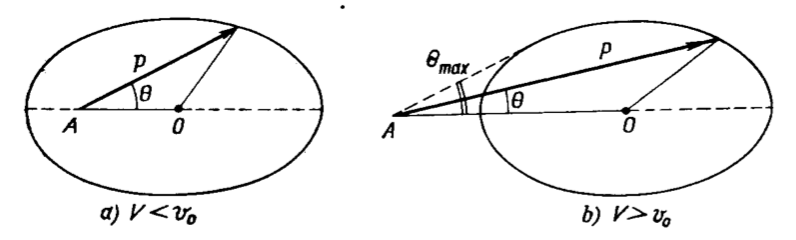
\includegraphics[scale=0.45]{ellisse}
\end{figure}
Le componenti del momento nel sistema del centro di massa si trasformano, secondo le trasformazioni di Lorentz, nel seguente modo nel sistema del laboratorio:
\[
p_x = \gamma(v)(p_0\cos\vartheta_0+E_0v) \quad p_y = p_0\sin\vartheta_0
\]
da cui, eguagliando ai soli termini in $\vartheta_0$, quadrando e sommando:
\[
\left( \frac{p_x-\gamma(v)E_0v}{\gamma(v)p_0} \right)^2+\left( \frac{p_y}{p_0} \right)^2=1
\]
Nello spazio dei momenti quest'equazione rappresenta un'ellisse centrata in $(\gamma(v)E_0v,0)$ (rappresentato in figura dal punto $O$, mentre $A$ rappresenta l'origine degli assi) con semiassi $\gamma(v)p_0$ e $p_0$. Quindi, se $v>p_0/E_0=v_0$ otteniamo che $O=(\gamma(v)E_0v,0)>(\gamma(v)p_0,0)$, cioè l'origine degli assi si trova all'esterno dell'ellisse e, a $\vartheta$ fissato, dunque, ci sono due possibili soluzioni. E' altrettanto chiaro che, in questo contesto, il valore dell'angolo $\vartheta$ non può superare un certo valore $\vartheta_{max}$. Tale valore può essere ricavato imponendo che il discriminante dell'equazione di partenza sia pari a 0. (il risultato del prof non mi torna ?????) Osserviamo infine che nel limite classico l'ellisse collassa in una circonferenza. 

\subsection{Effetto Compton relativistico}
Consideriamo un elettrone di quadrimomento 
\[
P^{\mu} = (E,\textbf{p})
\]
che collide con un fotone con quadrimpulso
\[
K^{\mu}=(E=h\nu, h\nu\hat{p})
\]
emergendo dalla collisione con, rispettivamente, $P'^{\mu}$ e $K'^{\mu}$. Supponiamo inoltre che l'angolo tra $\textbf{p}$ e $\hat{p}$ nel sistema del laboratorio sia $\vartheta$, mentre l'angolo tra $\textbf{p}$ e $\hat{p}'$ sia $\chi$ ed infine quello tra $\textbf{p}'$ e $\hat{p}'$ sia $\chi'$. Per conservazione del quadrimpulso scriviamo:
\[
P^{\mu}+K^{\mu}-K'{\mu}=P'{\mu}
\]
da cui, quadrando l'equazione
\[
-m^2+2P_{\mu}(K^{\mu}-K'^{\mu})-2K_{\mu}K'^{\mu}=-m^2
\]
\[
P_{\mu}(K^{\mu}-K'^{\mu})=K_{\mu}K'^{\mu}
\]
Osserviamo che:
\[
\begin{cases}
K_{\mu}K'^{\mu}=-h^2\nu\nu'+h^2\nu\nu'\cos\vartheta=-h^2\nu\nu'(1-\cos\vartheta) \\
P_{\mu}K^{\mu} = -Eh\nu+h\nu p\cos\chi \\
P_{\mu}K'^{\mu} = -Eh\nu' + h\nu'p\cos\chi'
\end{cases}
\]
quindi
\[
Eh(\nu-\nu')=hp(\nu'\cos\chi'-\nu\cos\chi)-2h^2\nu\nu'\sin^2\vartheta
\]
(non vengono i conti dei casi particolari ?????)
\section{Il momento angolare}
Definiamo, in analogia con il caso non relativistico, il tensore di rango 2 antisimmetrico \textbf{momento angolare} come
\[
L^{\mu\nu}=x^{\mu}P^{\nu}-x^{\nu}P^{\mu}=: x^{[\mu}P^{\nu]}
\]
Osserviamo immediatamente che
\[
\frac{dL^{\mu\nu}}{d\tau}=U^{[\mu}P^{\nu]}=mU^{[\mu}U^{\nu]}=0
\]
Possiamo definire inoltre il \textbf{momento angolare totale} per un sistema di particelle, sommando su un iperpiano di simultaneità i momenti angolari delle singole particelle:
\[
L_T^{\mu\nu}=\sum_n L_n^{\mu\nu}
\]
Chiaramente sarà necessario fissare un origine per il calcolo di $L$, e conseguentemente
\[
L^{\mu\nu}_T=L^{\mu\nu}_T(\Sigma,O)
\]
(manca anche tutta la parte sul centroide ecc.)
\subsection{Precessione di Thomas}
(??)

\chapter{Elettrodinamica covariante}
E' ben noto che i campi elettromagnetici obbediscono alle equazioni di Maxwell. La prima coppia di queste equazioni (in CGS)
\begin{equation}\label{eq:1max}
\boldsymbol{\nabla}\times \textbf{E} = -\frac{1}{c}\frac{\partial \textbf{B}}{\partial t} \text{ ,}\qquad \boldsymbol{\nabla}\cdot \textbf{B} = 0
\end{equation}
è equivalente al fatto che i campi derivano da dei potenziali $\textbf{A}$ e $\phi$, secondo le formule
\begin{equation}\label{eq:potenziali}
\textbf{E}=-\boldsymbol{\nabla}\phi-\frac{1}{c}\frac{\partial \textbf{A}}{\partial t} \text{ ,} \qquad \textbf{B}=\boldsymbol{\nabla}\times \textbf{A}
\end{equation}
La seconda coppia introduce l'interazione con le sorgenti dei campi, che sono le cariche e elettriche e le correnti:
\begin{equation}\label{eq:2max}
\boldsymbol{\nabla}\times \textbf{B} = \frac{1}{c}\frac{\partial \textbf{E}}{\partial t}+\frac{4\pi}{c}\textbf{J} \text{ ,} \qquad \boldsymbol{\nabla}\cdot \textbf{E}=4\pi\varrho
\end{equation}
Una conseguenza delle equazioni (\ref{eq:1max}) e (\ref{eq:2max}) è la la seguente equazione di continuità
\begin{equation}\label{eq:cons}
\frac{\partial \varrho}{\partial t}+\boldsymbol{\nabla}\cdot \textbf{J} = 0
\end{equation}

\section{Equazioni in forma covariante}
Per studiare la covarianza delle equazioni (\ref{eq:1max}), (\ref{eq:2max}) e (\ref{eq:cons}) rispetto al gruppo di Lorentz, introduciamo il \textbf{quadripotenziale}
\begin{equation}
A^{\mu}=(\phi,\textbf{A}) \qquad A_{\mu} = (-\phi,\textbf{A})
\end{equation}
Data l'esistenza di una simmetria di Gauge nella teoria elettrodinamica, si ha che tale vettore trasforma come un quadrivettore a meno di una trasformazione di Gauge:
\[
\begin{cases}
A'^{\mu}(\textbf{x}') = \Lambda_{\nu}^{\mu}A^{\nu}(\textbf{x})+\partial^{\mu}\Theta \\
x'^{i} = \Lambda_{j}^{i} x^{j} \\
\end{cases}
\]
Nel seguito di queste note ignoreremo la possibilità di compiere trasformazioni di Gauge, e tratteremo di conseguenza $A^{\mu}$ come se fosse genuinamente un quadrivettore. Introduciamo anche il tensore antisimmetrico
\begin{equation}
F_{\mu\nu} = \partial_{\mu}A_{\nu}-\partial_{\nu}A_{\mu}
\end{equation}
Questo risulta evidentemente Gauge invariante, e conseguentemente è a tutti gli effetti un tensore. Le sue componenti trasformano secondo l'equazione (3.6):
\[
\begin{cases}
F'_{\mu\nu}(\textbf{x}') = (\Lambda^{-1})_{\mu}^{\alpha}(\Lambda^{-1})_{\nu}^{\beta}F_{\alpha\beta}(\textbf{x}) \\
x'^{i} = \Lambda_{j}^{i} x^{j} \\
\end{cases}
\]
Il confronto con la (\ref{eq:potenziali}) porta alle seguenti componenti:
\[
F_{j0}=\partial_j A_0 -\partial_0A_j = -\partial_j A^0 +\partial_0 A^j=-\partial_j\phi -\frac{1}{c}\frac{\partial A_j}{\partial t}=E_j
\]
\[
F_{ij}\overset{i,j\not=0}{=} \partial_iA_j -\partial_jA_i = e_{ijk}B_k
\]
Esplicitamente possiamo scrivere:
\[
F_{\mu\nu}=
\left( \begin{array}{cccc}
0 & -E_x & -E_y & -E_z \\
Ex & 0 & B_z & -B_y \\
E_y & -B_z & 0 & B_x \\
E_z & B_y & -B_x& 0 \\
\end{array}\right)
\]
Da questo si verifica immediatamente che la prima coppia di equazioni di Maxwell è identica alle equazioni
\begin{equation}\label{eq:1cov_max}
e^{\alpha\beta\mu\nu}\partial_{\beta}F_{\mu\nu}=0
\end{equation}
esprimibile anche come:
\[
\sum_{\text{ciclica}}\partial_{\beta}F_{\mu\nu} := \partial_{\beta}F_{\mu\nu}+\partial_{\nu}F_{\beta\nu}+\partial_{\mu}F_{\beta\nu}=0
\]
Questo significa che possiamo concludere la covarianza delle equazioni (\ref{eq:1max}) grazie al fatto che $F_{\mu\nu}$ è un tensore nello spazio di Minkowsky. 
\\ (questione forma esatta e chiusa?????)
\\
Per mostrare la covarianza anche della successiva coppia di equazioni, introduciamo formalmente la corrente quadridimensionale, di componenti
\[
J^{\mu} = (c\varrho, \textbf{J})
\]
E' ovviamente verificata a seguente identità nel caso in cui $J^{\mu}$ risulti effettivamente un quadrivettore:
\[
\partial_{\mu}J^{\mu}=0
\]
che risulta essere la riscrittura covariante dell'equazione di continuità. Inoltre, si verifica direttamente dalla definizione di $F_{\mu\nu}$ che
\begin{equation}
\partial_{\nu}F^{\mu\nu} = -\frac{4\pi}{c}J^{\mu}
\end{equation}
è una riscrittura covariante di (\ref{eq:2max}). 

\subsection{Corrente elettrica}
Mostriamo ora che siamo in grado di dare una definizione di corrente elettrica che renda $J^{\mu}$ un quadrivettore. Consideriamo una carica puntiforme $e$, e sia $z^{\mu}(\tau)$ la sua linea di universo, parametrizzata, ad esempio, con il tempo proprio $\tau$. Se la carica è invariante per trasformazioni di Lorentz, allora l'integrale esteso alla linea di universo
\[
J^{\mu}(x) = e\int \delta^{(4)}(x^{\mu}-z^{\mu}(\tau) )dz^{\mu}
\]
definisce un campo di quadrivettori che chiameremo \textbf{quadricorrente elettrica}. Chiaramente con $\delta^{(4)}$ si intende
\[
\delta^{(4)}(x) = \delta(t)\delta(x^1)\delta(x^2)\delta(x^3)
\]
determinata univocamente dalla proprietà
\[
\int \delta^{(4)}(x-y)f(y) d^4x = f(x)
\]
Osserviamo che tale integrale è invariante per riparametrizzazioni. Infatti, sia $p=p(\tau)$ una funzione invertibile. Allora: (ci provo eh!)
\[
dz^{\mu}(\tau) = \frac{\partial z^{\mu}}{\partial \tau}d\tau
\]
\[
dz^{\mu}(p(\tau))=\frac{\partial z^{\mu}}{\partial p}dp=\frac{\partial z^{\mu}}{\partial p(\tau)}dp(\tau) = \frac{\partial z^{\mu}}{\partial \tau}\frac{\partial \tau}{\partial p}\frac{\partial p}{\partial \tau}d\tau = dz^{\mu}(\tau)
\]
Conseguentemente, possiamo scegliere $p=x^0$, in modo tale che $z^0(x^0)=x^0=t$. Otteniamo
\[
J^{\mu}(x) = e\int \delta^{(4)}(x^{\mu}-z^{\mu})dz^{\mu}(t)=e\int \delta^{(4)}(x^{\mu}-z^{\mu}(t))\frac{dz^{\mu}}{dt}dt
\]
Ora, l'integrale in $dt$ integra la componente temporale della delta ed il risultato è dunque
\begin{equation}\label{eq:dens}
J^{\mu}(t,\textbf{x}) = e\delta^{(3)}(\textbf{x}-\textbf{z}(t))v^{\mu}
\end{equation}
dove $v^{\mu}=dz^{\mu}/dt=(1,\textbf{v}(t))$. La definizione (\ref{eq:dens}) come corrente elettrica è innanzitutto giustificata dal fatto che $J^{\mu}$ soddisfa l'equazione di continuità. Infatti, consideriamo $J^0(t,\textbf{x})=e\delta^{(3)}(\textbf{x}-\textbf{z}(t))$ e scriviamo:
\[
\frac{\partial J^0}{\partial t}=-ev^i\frac{\partial}{\partial x^i}\delta^{(3)}(\textbf{x}-\textbf{z}(t))=-\frac{\partial J^i}{dx^i}
\]
cioè $\partial_{\mu}J^{\mu}=0$ è soddisfatta. Inoltre, $J^0$ rappresenta la carica elettrica. Infatti, per le proprietà della delta:
\[
\int J^0(t,\textbf{x})d\textbf{x}=e\int \delta^{(3)}(\textbf{x}-\textbf{z}(t))v^{\mu}d\textbf{x}=e
\]
L'invarianza di Lorentz della carica dell'elettrone è resa necessaria dal principio di relatività, perchè la carica elettrica è la sorgente dei campi elettromagnetici e, dunque, misure dei campi potrebbero rivelare la velocità del sistema di riferimento. Più concretamente, una dipendenza della carica dell'elettrone dalla velocità è sicuramente inammissibile, perchè altrimenti non sarebbe possibile avere atomi elettricamente neutri. Inoltre, gli spettri atomici sono indipendenti dalla velocità degli elettroni negli atomi, e dipendono dalla velocità di questi ultimi solo attraverso l'effetto Doppler. \\
Data l'additività della carica, la corrente di un sistema di particelle potrò essere scritta come
\begin{equation}
J^{\mu}(t,\textbf{x})=\sum_n e_n \delta^{(3)}(\textbf{x}-\textbf{z}_n(t))v^{\mu}_n
\end{equation}
Vogliamo mostrare ora la legge di conservazione relativistica della carica elettrica. Per farlo, consideriamo due iperpiani di simultaneità $\Sigma_1$ e $\Sigma_2$. Mandando all'infinito i loro estremi possiamo scrivere il seguente integrale:
\[
0=\int \partial_{\mu}J^{\mu}d^4x=\int_{\Sigma_2}J^0(t_2,\textbf{x})d^3x-\int_{\Sigma_1}J^0(t_1,\textbf{x})d^3x+\int_{t_1}^{t_2}dt \int d^3x \boldsymbol{\nabla}\cdot\textbf{J}(\textbf{x},t)
\]
Osserviamo che se $\textbf{J}$ tende a zero all'infinito in maniera opportunamente rapida, una volta definita
\[
q:=\int_{\Sigma}J^0(t,\textbf{x})d^3x
\]
che chiameremo \textbf{carica elettrica}, otteniamo la legge di conservazione
\begin{equation}
q(t_1)=\int_{\Sigma_2}J^0(t_2,\textbf{x})d^3x = \int_{\Sigma_1}J^0(t_1,\textbf{x})d^3x = q(t_2)
\end{equation}
Questo significa che se $J^{\mu}$ è un quadrivettore, allora $q(t)$ è uno scalare di Lorentz, e conseguentemente invariante. Più in generale, consideriamo il fatto che $N_{\mu}=(-1,0,0,0)$ è il quadrivettore normale all'iperpiano $\Sigma_1$ e $N'_{\mu}=(1,0,0,0)$ quello normale a $\Sigma_2$. Quindi:
\[
q=\int_{\Sigma_1}J^0(t,\textbf{x})d^3x=-\int_{\Sigma_1}J^{\mu}N_{\mu}dV=\int_{\Sigma_2} J^{\mu}N'_{\mu}dV'=\int_{\Sigma_2}J'^{\mu}N'_{\mu}dV'=q'
\]
Possiamo costruire un teorema di Gauss in 4 dimensioni, in modo da rendere più generali le espressioni che abbiamo precedentemente discusso. A tale scopo, indichiamo con $\partial \Omega$ il bordo orientato della regione $\Omega$. Assumeremo che $\partial \Omega$ sia unione disgiunta di certe ipersuperfici, alcune delle quali sono spacelike (il quadrivettore normale è di tipo tempo), altre timelike (viceversa), ma mai lightlike. Sia $N_{\mu}$ il vettore normale al bordo, orientato verso l'esterno di $\Omega$ sui tratti di $\partial \Omega$ che sono di tipo tempo, e verso l'interno sui tratti spacelike. Infine, sia $K^{\Xi \nu}$ un tensore, dove $\Xi$ indica gli altri indici possibilmente presenti. Allora:
\begin{equation}
\int_{\Omega} \partial_{\mu}K^{\Xi \mu}d^4x = \int_{\partial\Omega}K^{\Xi\mu}N_{\mu}dV
\end{equation}
dove $dV$ è l'elemento di volume sul bordo. In generale
\[
dV=N^{\mu}e_{\mu\alpha\beta\gamma}dx^{\alpha}dx^{\beta}dx^{\gamma}
\]

\subsection{Trasformazione dei campi}
da fare

\subsection{Simmetrie locali}
Consideriamo un campo scalare complesso $\phi(z)$ che obbedisca all'equazione di Klein-Gordon:
\[
\eta^{\mu\nu}\partial_{\mu}\partial_{\nu}\phi(z)-m^2\phi(z)=0
\]
Una trasformazione di Gauge del tipo
\[
\begin{cases}
\phi' = e^{i\alpha}\phi \\
\overline{\phi}'=e^{-i\alpha}\overline{\phi}\\
\end{cases}
\]
lascia invariate le equazioni del moto. Conseguentemente, il gruppo di simmetria globale del sistema è $U(1)$, cioè il gruppo delle matrici unitarie $n\times n$, omeomorfo al \textbf{gruppo unitario}, cioè il cerchio unitario nel piano complesso. \\
Potremmo però essere interessati ad una trasformazione di Gauge locale, ovvero introdurre una fase dipendente dalla posizione:
\[
\begin{cases}
\phi' = e^{i\alpha(z)}\phi \\
\overline{\phi}'=e^{-i\alpha(z)}\overline{\phi}\\
\end{cases}
\]
Questa trasformazione rompe però la simmetria. Infatti:
\[
\partial _{\mu}\phi' = e^{i\alpha(z)}\partial_{\mu}\phi(z)+ie^{i\alpha(z)}\phi(z)\partial_{\mu}\alpha(z)
\]
Di conseguenza, per far sì che la simmetria locale non venga rotta, è necessario introdurre un campo che non sia invariante di Gauge, ma la cui trasformazione, anzi, mostri un termine dipendente dal gradiente della fase. Un campo del genere è il quadripotenziale:
\[
A'_{\mu}=A_{\mu}+\partial_{\mu}\alpha(z)
\]
Scriviamo allora, se $e$ è la carica dell'elettrone:
\[
ieA'_{\mu}\phi'=ie\left( A_{\mu}+\frac{1}{e}\partial_{\mu}\alpha(z) \right)\phi'
\]
e introduciamo la \textbf{derivata covariante} così definita
\[
\nabla_{\mu} \phi(z) = \partial_{\mu}\phi(z) - ieA_{\mu}\phi(z)
\]
Sostituendo le quadriderivate con la derivata covariante, allora, possiamo mantenere la simmetria locale per trasformazioni di Gauge dipendenti dal punto:
\[
\eta^{\mu\nu}\nabla_{\mu}\nabla_{\nu}\phi(z)-m^2\phi(z)=0
\]
Questa equazione introduce un accoppiamento tra il campo scalare complesso ed il campo elettromagnetico: questo significa che tutti i corpi descritti da un campo scalare complesso devono possedere una carica, in quanto esiste un'interazione con il campo elettromagnetico. E' necessario notare, però, che queste considerazioni non riguardano mai un teoria classica.

\chapter{Principi variazionali}
Allo scopo di costruire teorie invarianti di Lorentz, è estremamente conveniente usare il principio variazionale di \textbf{minima azione}, in qui le equazioni del moto per campi $\phi$ si deducono dalla condizione di stazionarietà di un funzionale della forma
\begin{equation}
I[\phi] = \int \mathcal{L}(x)d^4x
\end{equation}
I campi $\phi$ hanno in generale molte componenti che indichiamo con $\phi_A(x)$ (dove per $x$ intenderemo sempre $x^{\mu}$), $I[\phi]$ viene detta \textbf{azione} ed $\mathcal{L}(x)$ \textbf{densità lagrangiana}. Per i nostri scopi, la Lagrangiana sarà sempre funzione dei campi
\[
\mathcal{L}(x) = \mathcal{L}(\phi_A(x), \partial_{\mu}\phi_A(x),x)
\]
equipaggiata con la seguente proprietà di invarianza relativistica: se indichiamo con $\phi'_A$ il campo risultante dalla trasformazione delle coordinate tramite un boost di Lorentz ed una traslazione otteniamo
\begin{align*}
\mathcal{L}'(x) &\equiv \mathcal{L}(\phi'_a(x), \partial_{\mu}\phi'_A(x), x) \\
&= \mathcal{L}(\phi_A(\Lambda^{-1}(x-a)), \partial_{\mu}\phi_A(\Lambda^{-1}(x-a)), \Lambda^{-1}(x-a)) \\ &= \mathcal{L}(\Lambda^{-1}(x-a))
\end{align*}
cioè è invariante di Lorentz. Tale richiesta è indispensabile, chiaramente, a garantire la covarianza delle equazioni del moto. Per traslazioni pure si ha $\Lambda=1$ e conseguentemente $\phi'_A(x) = \phi_A(x-a)$, da cui discende che la densità Lagrangiana non può dipendere esplicitamente dalle coordinate. 

\section{Equazioni di Eulero-Lagrange}
Se una piccola variazione $\delta\phi_A(x)$ di una data configurazione $\phi_A(x)$ non cambia il valore dell'azione al primo ordine in $\delta\phi_A(x)$, si dirà che l'azione è \textbf{stazionaria} nel \emph{punto} $\phi_A(x)$. Si ottiene in generale
\[
\delta I = \int \frac{\delta I}{\delta \phi_A(x)}\delta\phi_A(x)d^4x = 0
\]
dove $\delta I / \delta\phi_A(x)$ è detta \textbf{derivata variazionale} del funzionale $I$ e rappresenta in generale il coefficiente di $\delta\phi_A(x)$ nell'espressione della variazione prima $\delta I$. Il principio di minima azione risulta a questo punto equivalente alla richiesta
\begin{equation}\label{eq:staz}
\frac{\delta I}{\delta \phi_A(x)}=0
\end{equation}
Partendo da un'azione generica, possiamo esprimere la sua variazione come:
\[
\delta I = \int \left( \frac{\partial \mathcal{L}}{\partial \phi_A}\delta \phi_A +\frac{\partial \mathcal{L}}{\partial \partial_{\mu}\phi_A}\partial_{\mu}\delta\phi_A\right)d^4x
\]
In generale possiamo sempre scegliere variazioni arbitrarie a supporto compatto: in tal caso, riscriviamo il secondo termine come
\[
\int \frac{\partial \mathcal{L}}{\partial \partial_{\mu}\phi_A}\partial_{\mu}\delta\phi_Ad^4x = \int \partial_{\mu} \left( \frac{\partial \mathcal{L}}{\partial \partial_{\mu}\phi_A}\delta\phi_A \right)d^4x - \int \partial_{\mu} \left(\frac{\partial \mathcal{L}}{\partial \partial_{\mu}\phi_A} \right)\delta\phi_Ad^4x
\]
Ora, utilizzando il teorema di Gauss e richiedendo che il termine al bordo sia nullo otteniamo
\[
\int_{\Omega} \partial_{\mu} \left( \frac{\partial \mathcal{L}}{\partial \partial_{\mu}\phi_A}\delta\phi_A \right)d^4x = \int_{\partial\Omega} \frac{\partial \mathcal{L}}{\partial \partial_{\mu}\phi_A}\delta\phi_AN^{\mu}dV =0
\]
Di conseguenza possiamo riscrivere la variazione dell'azione come
\[
\delta I = \int \left( \frac{\partial \mathcal{L}}{\partial \phi_A} - \partial_{\mu} \frac{\partial \mathcal{L}}{\partial \partial_{\mu}\phi_A}  \right) \delta\phi_Ad^4x
\]
La condizione di stazionarietà (\ref{eq:staz}) richiede allora che
\[
\frac{\delta I}{\delta \phi_A(x)} \equiv \frac{\partial \mathcal{L}}{\partial \phi_A} - \partial_{\mu} \frac{\partial \mathcal{L}}{\partial \partial_{\mu}\phi_A}  = 0
\]
Queste sono le \textbf{equazioni di Eulero-Lagrange} per i campi, ed una teoria contraddistinta da un'equazione di questo tipo viene detta \textbf{teoria di campo a 3+1 dimensioni}. Possiamo notare subito che riducendosi ad una teoria in 0+1 dimensioni otteniamo 
\[
\frac{\partial L}{\partial q^i}-\frac{d}{dt}\frac{\partial L}{\partial \dot q^i}=0
\]
ovvero le equazioni di Eulero-Lagrange della meccanica classica. Chiaramente $L$ non è più una densità Lagrangiana, in quanto l'integrazione sullo spazio di una tale funzione perde di significato. \\
La densità Lagrangiana non è univocamente determinata. Infatti, la seguente trasformazione
\[
\mathcal{L}_1(x) = \mathcal{L}(x)+\partial_{\mu}\mathcal{F}^{\mu}(x)
\]
non modifica le equazioni del moto. 

\subsection{Campo scalare}
Consideriamo l'equazione di Klein-Gordon:
\[
\partial^{\mu}\partial_{\mu}\phi-m^2\phi=0
\]
Possiamo fare in modo che quest'equazione discenda da un principio di minima azione? Prendiamo spunto dal caso 0+1 dimensionale, dove l'equazione assume la seguente forma 
\[
\ddot q+m^2q=0
\]
ovvero quella di un'equazione armonica. La Lagrangiana corrispondente ad una tale equazione è data da:
\[
L = \frac{1}{2}\dot q^2 - \frac{m^2}{2}q^2
\]
Conseguentemente scegliamo di scrivere la seguente densità Lagrangiana per l'equazione di Klein-Gordon:
\[
\mathcal{L} = \frac{1}{2}\partial_{\mu}\partial^{\mu}\phi -\frac{m^2}{2}\phi^2
\]
Dalle equazioni di Eulero-Lagrange otteniamo
\[
- \partial_{\mu} \frac{\partial \mathcal{L}}{\partial \partial_{\mu}\phi} = -\partial_{\mu}\partial^{\mu}\phi \qquad \frac{\partial \mathcal{L}}{\partial \phi}=-m^2\phi
\]
Deduciamo da ciò che la densità Lagrangiana corretta debba essere
\[
L = -\frac{1}{2}\dot q^2 - \frac{m^2}{2}q^2
\]
Sulla base di questi argomenti possiamo costruire la densità Lagrangiana anche dell'oscillatore anarmonico
\[
\mathcal{L}=-\frac{1}{2}\eta^{\mu\nu}\partial_{\mu}\partial_{\nu}\phi-\frac{m^2}{2}\phi^2 -V(\phi)
\]
che conduce all'equazione di Klein-Gordon non lineare
\[
\partial^{\mu}\partial_{\mu}\phi-m^2\phi=\frac{\partial V(\phi)}{\partial\phi}
\]
\subsection{Azione per una particella}
Il moto della particella libera può essere ricavato da un principio variazionale che ha un suo interesse particolare. Infatti l'azione di un sistema libero è il punto di partenza per l'introduzione delle interazioni. Cerchiamo un'azione che sia invariante di Lorentz: per una particella si massa $m$ si può considerare ad esempio
\[
I[x^{\mu}(\tau)] = \alpha \int _{x_1}^{x_2}d\tau
\]
dove la costante $\alpha$ deve essere un'energia per rispettare le dimensioni ed $x_1$, $x_2$ sono eventi nello spazio-tempo connessi tramite una curva timelike. Scegliendo $\alpha=-m$ (nel caso $c=1$) si ottiene la seguente azione
\[
I[x^{\mu}(\tau)] = -m\int_{x_1}^{x_2}\sqrt{-dx^{\mu}dx_{\mu}}
\]
Una variazione al primo ordine in $\delta x^{\mu}$ porta a:
\[
\delta I = -m\int_{x_1}^{x_2}\delta\sqrt{-dx^{\mu}dx_{\mu}}
\]
dove 
\[
\delta\sqrt{-dx^{\mu}dx_{\mu}} = \frac{1}{2}\frac{(-2)}{\sqrt{-dx^{\mu}dx_{\mu}}}\delta( dx^{\mu})dx_{\mu} = -\frac{dx^{\mu}}{d\tau}d(\delta x^{\mu})
\]
Di conseguenza
\begin{align*}
\delta I &= m\int_{x_1}^{x_2}\frac{dx^{\mu}}{d\tau}d \delta x^{\mu} = m\int_{x_1}^{x_2} d\left( \frac{dx^{\mu}}{d\tau}d \delta x^{\mu} \right) - m\int_{x_1}^{x_2} d\left( \frac{dx^{\mu}}{d\tau}\right)\delta x^{\mu} \\
&=\left. P_{\mu}\delta x^{\mu} \right| _{x_1}^{x_2}-\int_{x_1}^{x_2}\frac{dP^{\mu}}{d\tau}\delta x^{\mu} = 0
\end{align*}
Imponendo che le variazioni risultino nulle negli estremi della curva, la condizione estremale $\delta I=0$ equivale all'equazione del moto
\[
\dot P^{\mu}=0
\]

\section{Azione per il campo elettromagnetico}
Vogliamo scrivere l'azione per il campo elettromagnetico nella seguente forma:
\[
I = \int d^4 x \mathcal{L}_{EM}(F_{\mu\nu}, A_{\mu}) + I_{M} + I_{INT}
\]
Per farlo, osserviamo innanzitutto che le equazioni di Maxwell sono del primo ordine nei campi elettromagnetici e del secondo ordine nei potenziali $A_{\mu}$, e conseguentemente considereremo le componenti del campo $A_{\mu}(x)$ come le variabili dinamiche della teoria (ovvero le \emph{coordinate generalizzate}). Esistono due invarianti quadratici che si possono costruire con il tensore $F_{\mu\nu}$, ovvero:
\[
F^2 := F_{\mu\nu}F^{\mu\nu} = 2(\textbf{B}^2-\textbf{E}^2) \qquad ^*F^{\mu\nu}F_{\mu\nu} = 2\textbf{E}\cdot\textbf{B}
\]
dove abbiamo definito
\[
^*F^{\mu\nu}=\frac{1}{2}e^{\mu\nu\alpha\beta}F_{\alpha\beta}
\]
Osserviamo che quest'ultimo invariante può essere riscritto come una divergenza:
\begin{align*}
^*F^{\mu\nu}F_{\mu\nu} &=\frac{1}{2}e^{\mu\nu\alpha\beta}F_{\mu\nu}F_{\alpha\beta}=\frac{1}{2}e^{\mu\nu\alpha\beta}F_{\alpha\beta}(\partial_{\mu}A_{\nu}-\partial_{\nu}A_{\mu}) \overset{(*)}{=}e^{\mu\nu\alpha\beta}F_{\alpha\beta}\partial_{\mu}A_{\nu} = \\
&=\partial_{\mu}(e^{\mu\nu\alpha\beta}F_{\alpha\beta}A_{\nu}) - e^{\mu\nu\alpha\beta}A_{\nu}\partial_{\mu}F_{\alpha\beta} = \partial_{\mu}(e^{\mu\nu\alpha\beta}F_{\alpha\beta}A_{\nu})
\end{align*}
Conseguentemente, dato il fatto che
\[
\int d^4x\partial_{\mu}\mathcal{O}^{\mu} = 0
\]
otteniamo che il secondo invariante non influisce sulla forma dell'azione. Scriviamo allora:
\[
\mathcal{L}_{EM} = -\frac{1}{16\pi}F_{\mu\nu}F^{\mu\nu}
\]
dove il fattore di normalizzazione è dovuto alla nostra scelta di utilizzare la unità gaussiane non normalizzate. Dato il fatto che $\mathcal{L}_{EM}$ non contiene le cariche elettriche, interpreteremo tale funzione come la densità lagrangiana per il campo elettromagnetico libero. L'azione per l'interazione con il campo la scriveremo supponendo che la corrente $J^{\mu}$ non dipenda dal quadripotenziale:
\[
I_{INT} = \int d^4 x J^{\mu}A_{\mu}
\]
$I_{INT}$ risulta essere invariante di gauge. Infatti, considerando la trasformazione $A_{\mu} \to A_{\mu} + \partial_{\mu}\psi$ otteniamo
\begin{align*}
I_{INT} &= \int d^4x(A_{\mu}+\partial_{\mu}\psi)J^{\mu} = \int d^4 x A_{\mu}J^{\mu}+\int d^4x J^{\mu}\partial_{\mu}\psi \\
&=\int d^4 x A_{\mu}J^{\mu}+\int d^4 x \partial_{\mu}(\psi J^{\mu}) - \int d^4x \psi\partial_{\mu}J^{\mu}
\end{align*}
Ora, valendo $\partial_{\mu}J^{\mu}=0$ e supponendo che $\psi$ si annulli rapidamente all'infinito, è evidente che l'azione $I_{INT}$ soddisfa l'invarianza di gauge. Ribaltando il discorso, possiamo vedere la conservazione della carica come conseguenza della stessa invarianza di gauge. Per quanto riguarda, infine, l'azione corrispondente alla materia elettricamente carica $I_M$, supporremo che questa non dipenda da $A_{\mu}(x)$. Tale azione non è altrettanto univocamente determinata come le precedenti, poichè ovviamente dipende dal modello di materia che si vuole adottare. Per gli scopi dell'elettrodinamica classica, il modello a particelle puntiformi risulta sufficientemente adeguato. Di conseguenza, dato il risultato del paragrafo precedente:
\[
I_M = -\sum_n m_n \int _{\gamma_n}d\tau_n
\] 
essendo l'integrale esteso sulla linea di universo della carica corrispondente. Possiamo quindi riscrivere l'azione completa come:
\[
I[A^{\mu}]=-\frac{1}{16\pi}\int d^4 xF_{\mu\nu}F^{\mu\nu}+\int d^4x A_{\mu}J^{\mu} -\sum_n m_n \int _{\gamma_n}d\tau_n
\]
Consideriamo ora per prima cosa la variazione al primo ordine di $I_{EM}$ in $A_{\mu}$, ottenendo:
\begin{align*}
\delta I_{EM} &= -\frac{1}{16\pi}\int d^4 x \delta(F_{\mu\nu}F^{\mu\nu}) = -\frac{1}{8\pi}\int d^4 x F^{\mu\nu}\delta F_{\mu\nu} = -\frac{1}{4\pi}\int d^4 x F^{\mu\nu}\partial_{\mu}\delta A_{\nu} = \\
&= -\frac{1}{4\pi}\int d^4 x\partial_{\mu}(F^{\mu\nu}\delta A_{\nu} ) + \frac{1}{4\pi}\int d^4x (\partial_{\mu}F^{\mu\nu})\delta A_{\nu} = \frac{1}{4\pi}\int d^4x (\partial_{\mu}F^{\mu\nu})\delta A_{\nu}
\end{align*}
Conseguentemente, annullando la variazione al primo ordine in $A_{\mu}$ dell'azione totale si ottiene:
\[
0 = I[A_{\mu}+\delta A_{\mu}] - I[A_{\mu}] = \delta I = \frac{1}{4\pi}\int d^4x (\partial_{\mu}F^{\mu\nu})\delta A_{\nu} + \int d^4 x J^{\mu}\delta A_{\mu}
\]
da cui si ricava immediatamente
\[
\partial_{\mu}F^{\mu\nu}+4\pi J^{\mu}=0
\]
Ci ricordiamo ora che 
\[
J^{\mu}(x) = \sum_n e_n \int _{z_n}\delta^{(4)}(x^{\mu}-z_n^{\mu}(\tau) ) dz_n^{\mu}
\]
dove $z_n^{\mu}$ sono le linee di universo delle singole cariche, e conseguentemente possiamo riscrivere
\[
\int d^4x J^{\mu} A_{\mu} = \sum_n e_n \int_{z_n} dz_n^{\mu} \int A_{\mu}(x^{\mu}) \delta^{(4)}(x^{\mu}-z_n^{\mu}(\tau) ) d^4x = \sum_n e_n \int_{z_n} A_{\mu}(z_n^{\mu})dz_n^{\mu}
\]
Per quanto riguarda l'azione libera, $I_M$, se le particelle hanno massa non nulla possiamo adottare l'azione
\[
I_M = -\sum_n m_n \int _{z_n} \sqrt{-dz_n^{\mu}dz_{n\mu}}
\]
Questa picture ci suggerisce la possibilità di calcolare la variazione dell'azione non più rispetto ad $A_{\mu}$, quanto piuttosto rispetto a $z^{\mu}$. Conseguentemente, supponendo che le $z^{\mu}$ risultino nulle ai bordi delle traiettorie:
\[
0 = \delta I = -\sum_n m_n \int _{z_n} \delta\sqrt{-dz_n^{\mu}dz_{n\mu}} + \sum e_n \int_{z_n}\partial_{\nu}A_{\mu}\delta z_{n}^{\nu} + \sum_n e_n \int_{z_n}A_{\mu}d(\delta z_n^{\mu})
\]
Il terzo termine, tramite integrazione per parti e teorema di Gauss, può essere riscritto come:
\[
\sum_n e_n \int_{z_n}A_{\mu}d\delta z_n^{\nu} = -\sum_n e_n \int_{z_n} (dA_{\mu})\delta z_n^{\nu}
\]
Quindi riordinando gli utili due termini otteniamo (NON CHIARO!):
\[
\sum_n e_n \int_{z_n} ( \partial_{\nu}A_{\mu}\delta z_n^{\nu}dz_n^{\mu} -\partial_{\mu}A_{\nu}\delta z_n^{\nu}dz_n^{\mu} ) = \sum_n e_n \int_{z_n} F_{\nu\mu}(z_n) \delta z_n^{\nu}d z_n^{\mu}
\]
Possiamo a questo punto scambiare gli indici muti per ottenere
\[
\sum_n e_n \int_{z_n} F_{\mu\nu}(z_n) \delta z_n^{\mu}d z_n^{\nu}
\]
Ricordando inoltre, dal paragrafo precedente, che
\[
\delta\left( -m \int_{z_n} \sqrt{-dz_n^{\mu}dz_{n\mu}} \right) = -\int_{z_n}\frac{dP^{\mu}}{d\tau}\delta z_{\mu}d\tau
\]
possiamo infine esprimere la variazione totale come
\begin{align*}
0 = \delta I &= -\sum_n \left( \int_{z_n}\frac{dP^{\mu}}{d\tau}\delta z_{\mu}d\tau_n + e_n \int_{z_n}F_{\mu\nu}\frac{dz_n^{\nu}}{d\tau_n}\delta z_n^{\mu}d\tau_n  \right) = \\
&= -\sum_n \int_{z_n} d\tau_n \left[ -\frac{dP_n^{\mu}}{d\tau_n}+e_nF_{\mu\nu}U_n^{\nu} \right]\delta z_n^{\mu}
\end{align*}
Otteniamo cioè un'equazione del moto Lorentz-invariante (ovviamente: infatti l'azione è l'integrale di una densità lagrangiana covariante) per le cariche:
\[
\frac{dP_n^{\mu}}{d\tau_n}=e_nF^{\mu}_{\nu}U_n^{\nu}
\]
da cui si ricava, per una singola particella
\[
\gamma \frac{dU^{\mu}}{dt}=\frac{e}{m}F^{\mu}_{\nu}U^{\nu}
\]
e si deduce la generalizzazione relativistica della forza di Lorentz e l'equazione del lavoro:
\[
\frac{d\gamma v^i}{dt} = \frac{e}{m}(E_i+(\textbf{v}\times \textbf{B})^i) \qquad \gamma\frac{d\gamma}{dt} = \frac{e}{m}E_iv^i
\]
Osserviamo quindi che la relatività conserva in grembo il fatto che il campo magnetico non compie lavoro. 

\section{Il tensore energia-impulso}

\subsection{Il caso generale}

Se la densità lagrangiana $\mathcal{L}=\mathcal{L}(\phi_{A}, \partial\phi_{A})$ (dove $A$ è un insieme di indici) non dipende esplicitamente dalle coordinate, si ha:
\begin{align*}
\partial_{\mu}\mathcal{L} &= \frac{\partial\mathcal{L}}{\partial\phi_A}\partial_{\mu}\phi_A+\frac{\partial\mathcal{L}}{\partial\partial_{\mu}\phi_A}\partial_{\nu}\partial_{\mu}\phi_A = \\
&= \frac{\partial\mathcal{L}}{\partial\phi_A}\partial_{\mu}\phi_A + \partial_{\nu}\left( \frac{\partial\mathcal{L}}{\partial\partial_{\nu}\phi_A}\partial_{\mu}\phi_A \right) - \partial_{\nu}\left( \frac{\partial\mathcal{L}}{\partial\partial_{\nu}\phi_A} \right)\partial_{\mu}\phi_A = \\
&= \left(\frac{\partial\mathcal{L}}{\partial\phi_A} -  \partial_{\nu} \frac{\partial\mathcal{L}}{\partial\partial_{\nu}\phi_A} \right)\partial_{\mu}\phi_A + \partial_{\nu}\left( \frac{\partial\mathcal{L}}{\partial\partial_{\nu}\phi_A}\partial_{\mu}\phi_A \right)
\end{align*}
Nel paragrafo (7.1) avevamo affermato che 
\[
\frac{\delta I}{\delta\phi_A(x)} \equiv \frac{\partial\mathcal{L}}{\partial\phi_A} -  \partial_{\nu} \frac{\partial\mathcal{L}}{\partial\partial_{\nu}\phi_A}
\]
e dato il fatto che l'energia si conserva se e solo se sono soddisfatte le equazioni del moto di Eulero-Lagrange, che sono soddisfatte se e soltanto se $\frac{\delta I}{\delta\phi_A(x)}=0$, otteniamo la condizione che tutto ciò è equivalente al fatto che $\partial_{\mu}\mathcal{L}$ risulti essere una quadri-divergenza. Quindi, riscrivendo 
\[
\partial_{\mu}\mathcal{L} = \partial_{\nu}(\delta_{\mu}^{\nu}\mathcal{L})
\]
e definendo il tensore
\begin{equation}
T_{\mu}^{\nu} = \delta_{\mu}^{\nu}-\frac{\partial\mathcal{L}}{\partial\partial_{\nu}\phi_A}\partial_{\mu}\phi_A
\end{equation}
detto \textbf{tensore energia impulso canonico}, otteniamo le quattro equazioni
\begin{equation}\label{eq:7.4}
\partial_{\nu}T_{\mu}^{\nu}=0
\end{equation}
La legge \eqref{eq:7.4} è la legge di conservazione del tensore energia impulso. Possiamo osservare che:
\[
P_{\mu} = \int_{\Sigma} T^0_{\mu}(t,\textbf{x})d^3x
\]
relazione suggerita dal fatto che la componente $T^0_0$ del tensore è una densità di energia. Infatti:
\[
-T^0_0 = \partial_0\phi_A\frac{\partial\mathcal{L}}{\partial\partial_0\phi_A}-\mathcal{L}
\]
ricordando che l'energia ottenuta attraverso una Lagrangiana è pari a:
\[
E = \dot q \frac{\partial L}{\partial \dot q}-L
\]
Questo significa che, ripristinando $c$, $-cP^0$ è l'energia del sistema, in accordo con le proprietà generali del quadrimpulso. Osserviamo ora che in generale il tensore energia impulso non è simmetrico, ma anzi le sue proprietà di simmetria sono legate ad una caratteristica imporante di sistemi fisici. Scrivendo infatti
\[
T^{\mu\nu} = \eta^{\alpha\nu}T_{\alpha}^{\mu}
\]
possiamoo esplicitare il seguente prodotto antisimmetrico
\[
J^{0\mu\nu} = T^{0\mu}x^{\nu}-T^{0\nu}x^{\mu}
\]
che corrisponde ad una \textbf{densità di momento angolare}. Possiamo subito notare che, ricordando $\partial_{\alpha}x^{\nu} = \delta_{\alpha}^{\nu}$:
\begin{align*}
\partial_{\alpha}J^{\alpha\mu\nu} &= \partial_{\alpha}(T^{\alpha\mu}x^{\nu}-T^{\alpha\nu}x^{\mu}) = \partial_{\alpha}(T^{\alpha\mu}x^{\nu})-\partial_{\alpha}(T^{\alpha\nu}x^{\mu}) \\
&= x^{\nu}\partial_{\alpha}T^{\alpha\mu}+T^{\alpha\mu}\partial_{\alpha}x^{\mu} -x^{\mu}\partial_{\alpha}T^{\alpha\nu}-T^{\alpha\nu}\partial_{\alpha}x^{\mu} \\
&= \delta_{\alpha}^{\nu}T^{\alpha\mu} - \delta_{\alpha}^{\mu}T^{\alpha\nu} = T^{\nu\mu}-T^{\mu\nu}
\end{align*}
cioè
\[
\partial_{\alpha}J^{\alpha\mu\nu}= T^{\nu\mu}-T^{\mu\nu} = 0 \Longleftrightarrow T^{\mu\nu} \text{ è simmetrico}
\]
Da ciò deriva che il significato fisico dell'eventuale simmetria del tensore energia impulso è la conservazione del momento angolare orbitale. Tipicamente la simmetria non si manifesta quando il sistema contiene un momento angolare intrinseco (spin). 

\subsection{Ambiguità di $T^{\nu}_{\mu}$}
La non univocità della lagrangiana si riflette ovviamente sulla forma del tensore $T^{\nu}_{\mu}$. Oltre a questo, però, esiste anche un'ambiguità di carattere più profondo che vogliamo adesso descrivere. Consideriamo il nuovo tensore energia impulso
\begin{equation}
^1 T_{\nu}^{\mu}=T_{\mu}^{\nu}+\partial_{\alpha}\xi^{\alpha\mu\nu} \qquad \xi^{\alpha\mu\nu} = -\xi^{\mu\alpha\nu}
\end{equation}
Allora la legge di conservazione \eqref{eq:7.4} rimane valida. Infatti, sfruttando l'antisimmetria di $\xi$, detto \textbf{tensore di Rosenberg-Belinfante}, otteniamo:
\[
\partial_{\mu}(\partial_{\alpha}\xi^{\alpha\mu\nu}) = \partial_{\alpha}(\partial_{\mu}\xi^{\mu\alpha\nu}) = - \partial_{\mu}(\partial_{\alpha}\xi^{\alpha\mu\nu}) \Longrightarrow 2\partial_{\mu}(\partial_{\alpha}\xi^{\alpha\mu\nu}) = 0
\]
da cui
\[
\partial^{\mu} (^1 T_{\mu}^{\nu}) = \partial^{\mu} T_{\mu}^{\nu}
\]
Inoltre, dal teorema di Gauss segue che il quadrimpulso totale non cambia se $\xi^{\alpha\mu\nu}$ si annulla in maniera sufficientemente rapida da annullare il suo flusso attraverso i bordi all'infinito. L'ambiguità qui discussa del tensore energia impulso non è così \emph{deprecabile}, in quanto ci permetterà sempre di renderlo simmetrico. 

\subsection{Significato delle componenti}
Abbiamo già osservato nel primo paragrafo che $T^{00}$ rappresenta la densità di energia e $G^{k} \equiv c^{-1}T^{0k}$ la densità di quantità di moto. Scriviamo allora la seguente equazione di trasformazione:
\[
\partial_{\mu}T^{\mu 0}=0 \Longrightarrow \frac{1}{c}\frac{\partial T^{00}}{\partial t} = -\partial_i T^{i0}
\]
che integrata attraverso il teorema di Gauss produce
\[
\frac{\partial E(V)}{\partial t} = \frac{\partial}{\partial t} \int_{V} T^{00} d^3x = -c \int_{\partial V} T^{i0}n_idS
\]
permettendoci di interpretare $cT^{i0}\equiv S^i$ (il \textbf{vettore di Poynting}) come flusso di energia nella direzione i-esima, dato il fatto che $E(V)$ rappresenta l'energia contenuta nel volume $V$. Allo stesso modo possiamo scrivere:
\[
\frac{1}{c}\frac{\partial T^{0k}}{\partial t} = -\partial_i T^{ik}
\]
che integrata come in precedenza restituisce
\[
\frac{\partial P^k(V)}{\partial t} = - \int_{\partial V}T^{ik}n_i dS
\]
e dunque interpretiamo le componenti $T^{ik}$ come flusso della k-esima componente dell'impulso nell'i-esima direzione. Ci si riferisce a tali componenti come alla componenti del \textbf{tensore degli sforzi}, poichè il flusso di impulso attraverso una superficie determina la forza agente sulla medesima. 
\\
Per concludere, se consideriamo il vettore $\textbf{G}$ di componenti $G^k = c^{-1}T^{0k}$ ed il vettore $\textbf{S}$ di componenti $S^k = cT^{k0}$ possiamo scrivere, nel caso in cui il tensore energia impulso sia simmetrico
\[
\textbf{G}=\frac{1}{c^2}\textbf{S}
\]
risultato noto con il nome di \textbf{teorema di Planck}: \emph{ad ogni corrente di energia è associato un trasporto di quantità di moto}. Tale teorema è una generalizzazione dell'equivalenza massa-energia, estesa però ai campi.  

\subsection{Campo scalare}
La Lagrangiana che abbiamo considerato nel paragrafo (7.1.1) per un campo scalare può essere riscritta in una forma più generale, in cui il termine quadratico viene assorbito dal potenziale:
\[
\mathcal{L} = -\frac{1}{2}\partial_{\mu}\phi\partial^{\mu}\phi-V(\phi)
\]
(??)

\subsection{Campo elettromagnetico}
La Lagrangiana del campo elettromagnetico così come l'abbiamo scritta in precedenza è data da:
\[
\mathcal{L} = -\frac{1}{16\pi}F_{\mu\nu}F^{\mu\nu}
\]
Per calcolare la derivata di $\mathcal{L}$, scriviamo la variazione
\[
\delta \mathcal{L} = -\frac{1}{8\pi}F^{\mu\nu}\delta F_{\mu\nu}=-\frac{1}{8\pi}F^{\mu\nu}(\delta \partial_{\mu}A_{\nu} -\delta\partial_{\nu}A_{\mu} ) = -\frac{1}{4\pi}F^{\mu\nu}\delta\partial_{\mu}A_{\nu}
\]
da cui banalmente
\[
\frac{\partial \mathcal{L}}{\partial\partial_{\mu}A_{\alpha}}=-\frac{1}{4\pi}F^{\mu\alpha}
\]
Ciò significa che il tensore energia-impulso per il campo elettromagnetico è pari a:
\begin{equation}\label{eq:7.6}
T^{\mu}_{\nu} = -\frac{1}{16\pi}F_{\alpha\beta}F^{\alpha\beta}\delta^{\mu}_{\nu}+\frac{1}{4\pi}F^{\mu\alpha}\partial_{\nu}A_{\alpha}
\end{equation}
(dove è necessario ricordare che nella definizione, $\phi_A$ ha un set di indici $A$ generalmente diversi da $\mu$ e $\nu$). La non invarianza di Gauge di questo tensore è manifesta (dovuta al termine in $\partial_{\mu}A_{\nu}$), e altrettanto la sua non-simmetria. Conseguentemente la forma della \eqref{eq:7.6} non è soddisfacente. Ricordando però la libertà concessa dal tensore di Belinfante, possiamo arbitrariamente aggiungere un termine all'espressione e riscriverla come:
\begin{equation}\label{eq:7.7}
\begin{split}
T^{\mu}_{\nu} &= -\frac{1}{16\pi}F_{\alpha\beta}F^{\alpha\beta}\delta^{\mu}_{\nu}+\frac{1}{4\pi}F^{\mu\nu}\partial_{\mu}A_{\nu}-\frac{1}{4\pi}F^{\mu\alpha}\partial_{\alpha}A_{\nu}  \\
&= -\frac{1}{16\pi}F_{\alpha\beta}F^{\alpha\beta}\delta^{\mu}_{\nu}+\frac{1}{4\pi}F^{\mu\alpha}F_{\nu\alpha}
\end{split}
\end{equation}
Adesso il tensore è evidentemente simmetrico ed invariante di gauge. Analizziamo le sue componenti. Per prima cosa, la densità di energia è data da:
\[
T^{00} = -\frac{1}{16\pi}F_{\alpha\beta}F^{\alpha\beta}\delta^0_0 +\frac{1}{4\pi}F^{0\alpha}F_{0\alpha} = -\frac{1}{16\pi}2(\textbf{E}^2-\textbf{B}^2) + \frac{1}{4\pi}\textbf{E}^2 = \frac{1}{8\pi}(\textbf{E}^2+\textbf{B}^2)
\]
Il vettore di Poynting $\textbf{S}$ va scritto come (osservando da subito che $\delta_0^i =0$ visto che $i=1,2,3$):
\[
T^{i0} = \frac{1}{4\pi} e^{ik}B_iE_k = \frac{1}{4\pi}(\textbf{E}\times \textbf{B})
\]
Infine, il tensore degli sforzi, chiamato in questo caso \textbf{tensore degli sforzi di Maxwell}, assume la forma:
\[
T_{ik} = \frac{1}{4\pi}\left( \frac{1}{2}(\textbf{E}^2+\textbf{B}^2)\delta_{ik}-E_iE_k-B_iB_k \right)
\]
(perchè il quadrimomento non può essere spacelike?? Che cazzo significa tutta quella roba a pagina 72??) \\ \\
Possiamo osservare che se $\sigma$ è la superficie di un dielettrico con normale esterna $\textbf{n}$, la forza esercitata dal campo sull'elemento di superficie $d\sigma$ è
\[
df_i = -T_{ik}n_kd\sigma
\]
Per questo a volte è il tensore $\sigma_{ik}=-T_{ik}$ ad essere chiamato tensore degli sforzi di Maxwell. Infine, notiamo che il tensore $T^{\mu\nu}$ è conservato solo in assenza di cariche e correnti. Infatti, utilizzando le equazioni di Maxwell si ricava (ricordando che $\delta^{\mu}_{\nu}\partial_{\mu} = \partial_{\nu}$) :
\[
\partial_{\mu}T^{\mu}_{\nu} = \frac{1}{4\pi}\left( -\frac{1}{2}F_{\alpha\beta}\partial_{\nu}F^{\alpha\beta}+F^{\mu\alpha}\partial_{\mu}F_{\nu\alpha}+F_{\nu\alpha}\partial_{\mu} F^{\mu\nu} \right) 
\]
Ricordando le equazioni di Maxwell:
\[
\partial_{\mu}F^{\mu\alpha} = -4\pi J^{\alpha} \qquad \sum_{\text{ciclica}} \partial_{\nu}F^{\alpha\beta} = 0
\]
possiamo riscrivere
\[
\partial_{\mu}T_{\nu}^{\mu} = \frac{1}{4\pi} \left( \frac{1}{2\pi}F_{\alpha\beta}\partial_{\alpha}F^{\nu\beta}+\frac{1}{2}F_{\alpha\beta}\partial_{\beta}F^{\alpha\nu}+F_{\mu\nu}\partial_{\mu}F^{\nu\alpha}-4\pi F_{\nu\alpha}J^{\alpha} \right)
\]
Permutando gli indici si può dimostrare che i primi tre termini si cancellano vincendevolmente, e di conseguenza otteniamo
\begin{equation}\label{eq:7.8}
\partial_{\mu}T^{\mu}_{\nu} = -F_{\nu\alpha}J^{\alpha}
\end{equation}
La componente temporale della \eqref{eq:7.8} rappresenta l'equazione di bilancio energetico:
\[
\frac{\partial T^{00}}{\partial t}+\boldsymbol{\nabla}\cdot \textbf{S}=-\textbf{E}\cdot \textbf{J}
\]

\subsection{Fluido perfetto}
L'idrodinamica relativistica presenta un interesse di principio, perchè dovrebbe essere applicata non solo quando è relativistica la velocità macroscopica del fluido, ma anche quando è tale la velocità microscopica delle particelle che lo compongono.\\
Consideriamo $\mu=mn_0$ la \emph{densità di massa} del fluido, dove $n_0$ rappresenta il numero di particelle per unità di volume proprio (volume a riposo) del fluido, ed m la massa propria delle particelle. Se $\varepsilon$ è l'energia interna per unità di massa e $s$ l'entropia per unità di massa, vale, nel sistema di riferimento in quiete con il fluido, la relazione termodinamica:
\[
d\varepsilon = Tds + \frac{P}{\mu^2}d\mu
\] 
Se il moto del fluido è isoentropico (cioè $ds=0$), si possono allora pensare $P$ ed $\varepsilon$ come funzioni univoche di $\mu$. Allora scriviamo:
\[
\varrho = \mu +\mu\varepsilon(\mu) \qquad P=\mu^2\frac{d\varepsilon}{d\mu}
\]
Possiamo riscrivere la condizione di isoentropia, osservando che
\[
\varepsilon(\mu) = \frac{\varrho-\mu}{\mu} =\frac{\varrho}{\mu}-1 \Longrightarrow d\varepsilon = d\left( \frac{\varrho}{\mu} \right)
\]
Inoltre
\[
d\left( \frac{P}{\mu} \right) = -\frac{P}{\mu^2}d\mu +\frac{1}{\mu}dP \Longrightarrow  -\frac{P}{\mu^2}d\mu = d\left( \frac{P}{\mu} \right) - \frac{1}{\mu}dP
\]
Dunque
\begin{equation}\label{eq:7.9}
0 = Tds = d\left( \frac{\varrho+P}{\mu} \right) - \frac{1}{\mu}dP
\end{equation}
Utilizzeremo questa relazione a breve, ma determiniamo prima il tensore energia impulso del fluido isoentropico (o prfetto). Come abbiamo detto precedentemente, il flusso di momento attraverso un elemento di superficie $d\sigma$ equivale alla forza agente su tale elemento di superficie. Quindi $df_i = -T_{ik}d\sigma_{k}$ è la i-esima componente della forza agente. Introduciamo ora una sistema di riferimento in cui un dato volume di fluido è a riposo. In un tale sistema di riferimento è valida la legge di Pascal, ovvero: \emph{la pressione $P$ applicata su una qualunque parte del corpo è trasmessa equamente in tutte le direzioni ed è ovunque perpendicolare alla superficie su cui agisce}. Quindi possiamo scrivere $-T_{ik}d\sigma_{k} = Pd\sigma_{i}$, ovvero il tensore degli sforzi può essere scritto come $T_{ik} = -P\delta_{ik}$. Inoltre, indichiamo con $\rho$ la densità di energia. A questo punto il tensore energia impulso assume la forma:
\[
^0T^{\mu\nu} =
\left( \begin{array}{cccc}
\varrho & 0 & 0 & 0 \\
0 & P & 0 & 0 \\
0 & 0 & P & 0 \\
0 & 0 & 0 & P \\
\end{array}\right)
\]
Adesso, per estendere il tensore ad un qualsiasi sistema di riferimento, introduciamo la quadrivelocità $U^{\mu}$ per il moto macroscopico di un volumetto di fluido. Nel sistema di riferimento in quiete con il volumetto abbiamo ovviamente $U^{\mu}=(1,0)$, e la forma del nuovo tensore deve essere scelta in modo tale che si riduca alla matrice precedentemente presentata nel sistema in quiete. Cioè:
\begin{equation}
T^{\mu\nu} = (P+\varrho)U^{\nu}U^{\mu}+\eta^{\mu\nu}P
\end{equation}
Inoltre, siccome la traccia è invariante per cambi di base, si nota subito che
\[
T^{\mu\mu} = 3P-\varrho
\]
Le componenti del tensore sono fornite da:
\[
\begin{split}
&T^{00} = (\varrho+P)U^0U^0-P = \gamma^2(\varrho+P)-P= \frac{\varrho+v^2/c^2 P}{1-v^2/c^2} \\
&T^{0i} = (\varrho+P)U^0U^i+P\eta^{0i} = \frac{(\rho+P)v^i}{1-v^2/c^2} \\
&T^{jk} = \frac{\varrho + P}{1-v^2/c^2}\frac{v^jv^k}{c^2}+P\delta^{jk}
\end{split}
\]
Studiamo ore il limite non relativistico di queste componenti, con il seguente accorgimento: non è sufficiente ignorare i termini di ordine $v/c$ o superiori, ma è necessario notare che $\varrho$ contiene l'energia di quiete $\mu c^2$, che si sviluppa nel seguente modo:
\[
\mu = \mu_0\sqrt{1-\frac{v^2}{c^2}} \simeq \mu_0 -\frac{\mu_0v^2}{2c^2}
\]
dove $\mu_0$ è la densità di massa non relativistica. Inoltre sarà necessario notare che l'energia interna $\varepsilon(\mu)$ e la pressione sono indubbiamente trascurabili rispetto a $\mu c^2$. Dunque:
\begin{align*}
T^{00} &= \frac{(\mu c^2+\mu\varepsilon)+Pv^2/c^2}{1-v^2/c^2} \simeq \frac{\mu c^2+\mu\varepsilon}{1-v^2/c^2} = \frac{\mu_0c^2+\mu_0\varepsilon}{\sqrt{1-v^2/c^2}} \\
&\simeq (\mu_0c^2+\mu_0\varepsilon)\left( 1+\frac{1}{2}\frac{v^2}{c^2} \right) \simeq \mu_0c^2 +\mu_0\varepsilon + \frac{1}{2}\mu_0v^2
\end{align*}
\[
c^{-1}T^{0i} \simeq \frac{(\mu c^2+\mu\varepsilon)v^i/c^2}{1-v^2/c^2} = \frac{(\mu c^2+\mu\varepsilon)v^i/c^2}{1-v^2/c^2} \simeq (\mu_0c^2+\mu_0\varepsilon)\frac{v^i}{c^2}\left(1+\frac{1}{2}\frac{v^2}{c^2} \right) \simeq \mu_0 v^i
\]
\[
T^{ik} \simeq \mu_0v^{i}v^{k}+\delta^{ik}P
\]
Dunque le componenti non relativistiche del tensore energia-impulso, che coincidono esattamente con i risultati della meccanica dei fluidi non relativistica, per il fluido perfetto sono:
\begin{equation}
\begin{cases}
T^{00} - \mu_0c^2 \simeq \frac{1}{2}\mu_0v^2+\mu_0\varepsilon \\
c^{-1}T^{0i} \simeq \mu_0v^i \\
T^{ik} \simeq \mu_0v^{i}v^{k}+\delta^{ik}P \\
\end{cases}
\end{equation}
Quanto possiamo fare ore è ricavare le equazioni del moto attraverso la legge di conservazione del tensore energia-impulso
\[
\partial_{\mu}T^{\mu\nu}=0
\]
Otteniamo:
\[
0 = \partial_{\mu}\left[ (P+\varrho)U^{\nu}U^{\mu}+\eta^{\mu\nu}P \right]
\]
da cui, contraendo con $U^{\nu}$:
\[
-U^{\nu}\partial_{\nu}P = (\varrho+P)U^{\mu}U^{\nu}\partial_{\mu}U^{\nu}-\partial_{\mu}[ (\varrho+P)U^{\mu}]
\]
Ora, siccome $U^{\nu}\partial_{\mu}U^{\nu} = \partial_{\mu}(U_{\nu}U^{\nu})-U^{\nu}\partial_{\mu}U_{\nu}$, cioè $U_{\nu}\partial_{\mu}U^{\nu}=0$, otteniamo:
\[
\partial_{\mu}[(\varrho+P)U^{\mu}] = U^{\nu}\partial_{\nu}P
\]
Ciò significa che possiamo sostituire questo termine nell'equazione di partenza, giungendo a:
\begin{equation}
(P+\varrho)U^{\mu}\partial_{\mu}U^{\nu} = -\partial_{\nu}P-U^{\nu}U^{\mu}\partial_{\mu}P
\end{equation}
Questa equazione si riduce, nel limite non relativistico, all'equazione di Eulero. A questo punto non abbiamo ancora introdotto la richiesta di isoentropia. Per farlo, riscriviamo l'equazione (le ultime considerazioni non sono chiare!!) 

\subsection{Particella libera}
L'energia di una particella libera è $P^0 = m\gamma$, mentre la sua quantità di moto è data in componenti da $P^j = m\gamma v^j$. Estendendo ad un sistema di particelle libere immaginiamo definiamo la densità di quantità di moto come
\begin{equation}
T^{i0}(t,\textbf{x}) = \sum_n P^i_n(t)\delta^{(3)}(\textbf{x}-\textbf{z}_n(t))
\end{equation}
mentre la corrente come
\begin{equation}
T^{jk}(t,\textbf{x}) = \sum_n P_n^j(t)\frac{dz_n^k(t)}{dt}\delta^{(3)}(\textbf{x}-\textbf{z}_n(t))
\end{equation}
dove stiamo assumendo, attraverso l'utilizzo della delta, che la densità di massa sia unicamente distribuita sulla linee di universo della particelle. Le formule scritte sono le componenti del tensore
\begin{equation}
T^{\mu\nu} (t,\textbf{x})=\sum_n P_n^{\mu}v_n^{\nu}\delta^{(3)}(\textbf{x}-\textbf{z}_n(t)) \qquad v_n^{\nu} = \frac{dz_n^{\nu}}{dt}
\end{equation}
In generale possiamo supporre che le linee di universo siano parametrizzate attraverso un parametro invariante qualsiasi $p$, e dunque possiamo riscrivere l'identità precedente nella seguente maniera:
\[
T^{\mu\nu} = \sum_n \int dp \delta^{(4)}(x^{\mu}-z_n^{\mu}(p))P_n^{\mu}\frac{dz_n^{\nu}}{dp}
\]
La scrittura attuale rende esplicita la natura tensoriale di $T^{\mu\nu}$. Oppure, noto il fatto che
\[
P^{\mu}_n = E_n \frac{dz_n^{\mu}}{dt} 
\]
possiamo scrivere in maniera altrettanto utile
\begin{equation}\label{eq:7.16}
T^{\mu\nu}(t,\textbf{x}) = \sum_n \frac{P_n^{\mu}P_n^{\nu}}{E_n}\delta^{(3)}(\textbf{x}-\textbf{z}_n(t))
\end{equation}
da cui si evince immediatamente la simmetria del tensore. Dalla relazione \eqref{eq:7.16} ricaviamo immediatamente la traccia $T$:
\[
T\equiv T^{\mu\mu} = -\sum_n \frac{m_{0n}^2\sqrt{1-v_n^2}}{m_{0n}}\delta^{(3)}(\textbf{x}-\textbf{z}_n(t)) = -\sum_n m_{0n}\sqrt{1-v_n^2}\delta^{(3)}(\textbf{x}-\textbf{z}_n(t))
\]
La media spaziale sull'unità di volume è ottenibile come segue:
\[
\int T d^3x = -\sum_n m_{0n}\sqrt{1-v_n^2}
\]
ed è cioè negativa. \\
Quanto possiamo ora è calcolare la legge di conservazione del tensore energia impulso in due diversi casi: 
\begin{enumerate}[i.]
\item \emph{le particelle si muovono sotto l'azione di un campo elettromagnetico}: usando l'espressione del tensore parametrizzato rispetto al tempo proprio $\tau_n$ otteniamo:
\[
\partial_{\mu}T^{\mu\nu}(t,\textbf{x}) = 
\]

\end{enumerate}
\end{document}